% Header mit Deklarationen
\documentclass[%
	pdftex,%              PDFTex verwenden
	a4paper,%             A4 Papier
	twoside,%             Einseitig/ wzeiseitig
	bibtotoc,%    		Literaturverzeichnis einfügen bibtotocnumbered: nummeriert
	liststotoc,%		Verzeichnisse einbinden in toc
	idxtotoc,%            Index ins Verzeichnis einfügen
	halfparskip,%        Europäischer Satz mit abstand zwischen Absätzen
	%chapterprefix,%       Kapitel anschreiben als Kapitel
	headsepline,%         Linie nach Kopfzeile
	footsepline,%         Linie vor Fusszeile
	pointlessnumbers,%     Nummern ohne abschließenden Punkt
	12pt,%                 Grössere Schrift, besser lesbar am bildschrim
	bibliography=totoc,
	cleardoublepage=empty,
	index=totoc,
	listof=totoc,
]{scrreprt}


\usepackage[backend=bibtex,bibencoding=ascii,style=numeric,citestyle=numeric-comp,defernumbers=true]{biblatex} 

%
% Seitenränder
%
\usepackage{geometry}
\geometry{a4paper, top=30mm, left=30mm, right=20mm, bottom=25mm, headsep=10mm, footskip=10mm}



%
% Paket für Übersetzungen ins Deutsche
%
\usepackage[french,english,ngerman]{babel}

%
% Pakete um Latin1 Zeichnensätze verwenden zu können und die dazu
% passenden Schriften.
%
%\usepackage[latin1]{inputenc}
% UTF8 Kompatabilität
\usepackage[utf8]{inputenc}
\usepackage[T1]{fontenc}

%
% Paket für Quotes
%
\usepackage[babel,french=guillemets,german=quotes]{csquotes}

%
% Paket zum Erweitern der Tabelleneigenschaften
%
\usepackage{array}


%
% Paket für schönere Tabellen
%
\usepackage{booktabs}

%
% Paket um Grafiken einbetten zu können
%
\usepackage{graphicx}
\usepackage{subfigure}
\usepackage{float} % zum abstellen der float umgebung von Grafiken

%
% Spezielle Schrift im Koma-Script setzen.
%
\setkomafont{sectioning}{\normalfont\bfseries}
\setkomafont{captionlabel}{\normalfont\bfseries} 
\setkomafont{pagehead}{\normalfont\bfseries} % Kopfzeilenschrift
\setkomafont{descriptionlabel}{\normalfont\bfseries}

%
% Zeilenumbruch bei Bildbeschreibungen.
%
\setcapindent{1em}
%\setlength{\abovecaptionskip}{0pt}

\usepackage{fancyhdr}
\pagestyle{fancy}
%\fancyhead{}
%\fancyfoot{}
%\fancyhead[LE,RO]{\leftmark}
%\fancyhead[LO]{\rightmark}
%\fancyhead[RE]{\thepage}
%\fancyhead[R]{\leftmark}
\fancyhead[RE]{\leftmark}
\fancyhead[LO]{\rightmark}
\fancyfoot[C]{\thepage}
\fancyhead[RO]{
\includegraphics[width=75pt]{HM_Deu_CMYK_Graust}}
\fancyhead[LE]{\textsc{Diplomarbeit}}
\fancypagestyle{plain}{}
\renewcommand{\chaptermark}[1]{\markboth{\thechapter{} #1}{}}
\renewcommand{\sectionmark}[1]{\markright{\thesection{} #1}{}}
\setlength{\headheight}{37pt} 


%\usepackage{scrpage2}
%\pagestyle{scrheadings}
% Inhalt bis Section rechts und Chapter links
%\automark[section]{chapter}

% Mitte: leer
%\chead{}

%
% mathematische symbole aus dem AMS Paket.
%
\usepackage{amsmath}
\usepackage{amssymb}
\usepackage[fixamsmath, disallowspaces]{mathtools}

%
% Type 1 Fonts für bessere darstellung in PDF verwenden.
%
\usepackage{mathptmx}           % Times + passende Mathefonts
\usepackage[scaled=.92]{helvet} % skalierte Helvetica als \sfdefault
\usepackage{courier}            % Courier als \ttdefault

%
% Paket um Textteile drehen zu können
%
\usepackage{rotating}




%
%1 Glossaries / Verzeichnisse
%
\usepackage[nonumberlist,toc,nopostdot]{glossaries}
% Entferne alphabetische Gruppierung des Glossars
\renewcommand{\glsgroupskip}{}
\makeglossaries


%
% Paket um LIstings sauber zu formatieren.
%
\usepackage[savemem]{listings}
\lstloadlanguages{TeX}



%
% Neue Umgebungen
%
\newenvironment{ListChanges}%
	{\begin{list}{$\diamondsuit$}{}}%
	{\end{list}}

%
% aller Bilder werden im Unterverzeichnis figures gesucht:
%
\graphicspath{{bilder/}}


%
% Anführungsstriche mithilfe von \textss{-anzufuehrendes-}
%
\newcommand{\textss}[1]{"`#1"'}

%
% Strukturiertiefe bis subsubsection{} möglich
%
\setcounter{secnumdepth}{4}

%
% Dargestellte Strukturiertiefe im Inhaltsverzeichnis
%
\setcounter{tocdepth}{4}

%
% Zeilenabstand wird um den Faktor 1.5 verändert
%
%\renewcommand{\baselinestretch}{1.5}
\usepackage{setspace} %Zeilenabstand einstellbar



\usepackage{caption}


\DeclareUnicodeCharacter{00A0}{ }



\usepackage{verbatim}




%\newcommand{\submissiondate}{27. August 2015}
%\newcommand{\submissionmonthyear}{August 2015}


% Tabellenprogramm
\usepackage{tabularx}
\usepackage{multirow}

% Plotten von Tabellen
\usepackage[svgnames]{xcolor}
\usepackage{pgfplots}
\pgfplotsset{every axis/.append style={
thick,
tick style={thick}},
%width=10cm,
compat=1.12,
cycle list={Bihler1\\Bihler2\\green\\orange\\},
}
\usepgfplotslibrary{external}
\usetikzlibrary{pgfplots.groupplots}



\usepackage{siunitx}



\addto\captionsngerman{
\renewcommand{\figurename}{Abb.}
\renewcommand{\tablename}{Tab.}
%\renewcommand{\refname}{Quellenverzeichnis}
% \renewcommand{\bibname}{Quellenverzeichnis}
}




% Bihlerfarben
\definecolor{Bihler1}{RGB}{21, 78, 113}
\definecolor{Bihler2}{RGB}{146, 46, 46}




\usepackage[section]{placeins}

\usepackage{pdfpages}

\usepackage{lscape}


\usepackage{colortbl}






\usepackage{microtype}
%\overfullrule=2cm



\newcommand*\cleartoleftpage{%
  \clearpage
  \ifodd\value{page}\hbox{}\newpage\fi
}





\begin{comment}
%
% Paket für Links innerhalb des PDF Dokuments
%
\definecolor{LinkColor}{rgb}{0,0,0.5}
\usepackage[%
	pdftitle={Titel},% Titel der Diplomarbeit
	pdfauthor={Jens Schmelkus},% Autor(en)
	pdfcreator={LaTeX, LaTeX with hyperref and KOMA-Script},% Genutzte Programme
	pdfsubject={Diplomarbeit}, % Betreff
	pdfkeywords={Keywords}]{hyperref} % Keywords halt :-)
\hypersetup{colorlinks=false,% Definition der Links im PDF File
	linkcolor=LinkColor,%
	citecolor=LinkColor,%
	filecolor=LinkColor,%
	menucolor=LinkColor,%
	pagecolor=LinkColor,%
	urlcolor=LinkColor}
	
	
\definecolor{Colour1}{HTML}{1B9E77}
\definecolor{Colour2}{HTML}{D95F02}
\definecolor{Colour3}{HTML}{7570B3}
\definecolor{Colour4}{HTML}{E7298A}
\definecolor{Colour5}{HTML}{66A61E}
\definecolor{Colour6}{HTML}{E6AB02}
\definecolor{Colour7}{HTML}{A6761D}
\end{comment}

% Literaturverzeichnis
\bibliography{literatur/bib}

\begin{document}

% Römische Nummerierung für Sonderseiten, wie Verzeichnisse und Anhang
\pagenumbering{Roman}

% Titelblatt
\begin{titlepage}
\setcounter{page}{1}
%\thispagestyle {empty}
%\fancypagestyle{plain}{}
\begin{center}
%\vspace{2cm}
%\setlength{\headheight}{15pt}
\begin{figure}[h!]
\vspace{0cm}
\centering
% 
\includegraphics[width=0.6\textwidth]{graphics/HM_Deu_CMYK}

\includegraphics[width=0.8\textwidth]{bilder/Logos/FK03_CMYK_Block.png}
\\[0.8cm]
% \includegraphics[width=0.25\textwidth]{bilder/}
\end{figure}
\vspace{1.5cm}

{\fontsize{20}{60}\scshape Diplomarbeit} 
\\[1.1cm]

\begin{doublespace}
{\fontsize{30}{22}\selectfont \textbf{Konzeptionierung, Entwicklung und Erprobung der Bordelektronik eines unbemannten Kleinstflugzeuges}\par} 
\vspace{1.4cm}
\end{doublespace}

\title{Konzeptionierung, Entwicklung und Erprobung der Bordelektronik eines Unbemannten Kleinstflugzeuges}
\author{Jens Schmelkus}
\date{Dezember 2017}

{\fontsize{23}{60}\scshape Jens Schmelkus} 
\\[2.0cm]


\textbf{Betreuer}: Prof. Dr. Karl Siebold



% \textbf{Fakultät}: Fakultät für Maschinenbau, Fahrzeugtechnik, Flugzeugtechnik

\textbf{Studiengang}: Fahrzeugtechnik 

\textbf{Abgabe}: 22.01.2018

\vfill

% \colorbox{orange}{Name oben drüber Betreuer kleiner als meiner, Fakultät, keine Tabellenform, Diplomarbeit kleiner}

\end{center}
\end{titlepage}


\cleardoublepage\thispagestyle{empty}

% \chapter*{Eigenständigkeitserklärung}
% \markboth{Eigenständigkeitserklärung}{Eigenständigkeitserklärung}
\chapter*{Erklärung}\addcontentsline{toc}{chapter}{Erklärung}
\markboth{Erklärung}{Erklärung}

Hiermit wird erklärt, dass die Arbeit mit obigem Thema selbständig verfasst und noch nicht anderweitig für Prüfungszwecke vorgelegt wurde. Weiterhin sind keine anderen als die angegebenen Quellen oder Hilfsmittel verwendet und wörtliche sowie sinngemäße Zitate als solche gekennzeichnet worden. \\[2cm]
%\begin{tabularx}{\textwidth}{lX}
% München, den \_\_\_\_\_\_\_\_\_\_\_\_\_\_\_\_\_\_\_\_ \hspace{10 mm} & \_\_\_\_\_\_\_\_\_\_\_\_\_\_\_\_\_ \\[0.2cm]
% & \hspace{5 mm} {\footnotesize Jens Schmelkus}
%\end{tabularx}





\cleardoublepage

% % Die eidesstattliche Erklärung mit Unterschrift
\chapter*{Sperrvermerk}\addcontentsline{toc}{chapter}{Sperrvermerk}

Diese Diplomarbeit enthält vertrauliche Informationen. Sie darf nicht vervielfältigt oder auf elektronischem Weg verteilt werden. Einsichtnahme ist für einen Zeitraum von 5 Jahren ab Abgabe nur für Prüfungszwecke gestattet.




\clearpage

\chapter*{Zusammenfassung}\addcontentsline{toc}{chapter}{Zusammenfassung}


Die Firma Bihler entwickelt und produziert für ihre Stanz-Biegeautomaten NC-Aggregate. Mit diesen werden Werkzeuge präzise bedient, um Bauteile und Baugruppen in der Massenproduktion zu fertigen. Um zu vermeiden, dass es zu Funktionsfehlern bei den in Serie gefertigten NCAs kommt, wird durch Prüfen während des Produktionsprozesses versucht, derartige Probleme so weit wie möglich zu auszuschließen. Obwohl die Aggregate bereits ein Prüfverfahren durchlaufen, werden nicht alle gravierenden Fehler entdeckt. Deshalb wird das derzeitige Prüfen analysiert und es werden Vorschläge zu einer eventuell nötigen Überarbeitung entwickelt.


Hierzu wird der Aufbau der verschiedenen Varianten der NCAs dargestellt, die elektronische Ansteuerung unter Zuhilfenahme des Kurvengetriebes erläutert und die Fahrbewegung der NCAs im Trapez- und Dreiecksprofil aufgezeigt. Es wird festgestellt, dass Funktionsstörungen der NCAs die verschiedensten Ursachen haben und alle am Produktionsprozess Beteiligten damit konfrontiert sind.

Der derzeitige Testlauf auf einem Prüfstand integriert das Einlaufen der Aggregate und erfasst beim kompletten Ein- und Ausfahren der Pinole während eines bestimmten Testzyklus im Bewegungsprofil Trapez Stromstärke und verschiedene Temperaturwerte. Hierdurch können Fehler aber nicht zuverlässig aufgedeckt werden, zumal keine Standards für die funktionsspezifischen Eigenschaften der NCA vorhanden sind und es kein Dokumentationssystem zur Erfassung von Problemen und deren Rückmeldung an die entsprechenden Abteilungen gibt.


Nach einer Auseinandersetzung mit den Grundlagen von Prüfkonzepten und Testverfahren werden deshalb teilweise auf der Grundlage des bisherigen Testablaufs entwickelte Testverfahren geprüft und bewertet. Dabei darf bei allen Testkonzepten der ökonomische Aspekt nicht außer Acht gelassen werden.

Das bisher schon eingesetzte langsame Abfahren im Trapezprofil ist wenig geeignet, da die Einflüsse des Reglers nicht erkennen lassen, ob eine Schwergängigkeit vorliegt. 

Aufgrund der Versuche kann davon ausgegangen werden, dass man weitreichende Erkenntnisse zu etwaigen Störungen durch das Belasten der NCAs beim Betreiben erhält. Da sich Tests mit einem direkten Belasten der Achse durch Anhängen einer Last oder Fahren auf einen Widerstand nicht als praxistauglich erweisen, werden Messungen analysiert, die aufgrund des Fahrprofils die Achsen dynamisch belasten. 

So wird das Fahrprofil Polynom 5. Ordnung neu entwickelt und berechnet. 19 NCAs werden mit dem Fahrprofil Polynom 5. Ordnung und mit dem Fahrprofil Stufenprofil gemessen und daraus Mittelwertkuren und Standardabweichungen berechnet. Bei einer Achse wird hierbei axiales Spiel hoch signifikant erkannt. Es bietet sich an, die Verfahrprofile Stufenprofil und Polynom 5. Ordnung einzusetzen, denn mit ihnen können die Achsen bis an die Belastungsgrenzen belastet werden und es lässt sich axiales Spiel erkennen. Weiterhin lassen sich diese Messungen leicht in den vorhandenen Prüfablauf integrieren.



Voraussetzung ist, dass auf eine für das Steuern der Achsen in Tests geeignete Steuerung zurückgegriffen werden kann, die auch das Aufzeichnen und Analysieren von Daten unterstützt. Dies ist mit der derzeitigen, nicht für den Testbetrieb ausgelegten VC 1 Steuerung nur sehr eingeschränkt möglich.

Als weitere Testmöglichkeit werden Schwingungsmessungen untersucht. Hierbei werden zuerst die zu erwartenden Schwingungsfrequenzen berechnet. Anschließend werden Versuche durchgeführt, um die grundsätzliche Eignung von Schwingungsmessungen als geeignete Messmethode zu evaluieren. Eine Analyse der Versuchsergebnisse zeigt, dass Schwingungsmessungen dazu geeignet sind, um Funktionsstörungen an den NCAs zu erkennen. Jedoch müssen weiterführende Versuche durchgeführt werden, um standardisierte Tests zu entwickeln.

Mit der Erfassung von Temperaturwerten wie Motortemperatur oder der Temperatur an den NCAs mithilfe externer Sensoren könnten zwar aussagefähige Ergebnisse gewonnen werden. Jedoch ist die Entwicklung praxistauglicher Messverfahren sehr aufwendig und bringt im Vergleich zu den anderen als geeignet erscheinenden Messverfahren keine entscheidenden Vorteile.


%Die Messung von Temperaturwerten wie Motortemperatur oder die Temperaturmessung mithilfe von externen Sensoren an den NCA ist im Vergleich zu den anderen untersuchten Messmethoden schwierig in der Umsetzung zu aussagekräftigen Messverfahren.





%Zudem haben Volumenstromessungen am Kühlmittel ergeben, dass man auch diese Messungen zur Analyse des Kühlsystems heranziehen kann.

Zur Analyse des Kühlmitteldurchflusses innerhalb des Aggregats wird ein Kennwert entwickelt. Aus der  Messung mehrerer Aggregate wird wiederum ein Mittelwert und dessen Standardabweichung abgeleitet,  die für das Testen zur Verfügung stehen.

Die Ergebnisse der Arbeit schaffen die Grundlage, an Hand derer das Prüfverfahren überarbeitet werden kann.

%Die Ergebnisse der Arbeit schaffen die Grundlage, an Hand derer das Prüfverfahren überarbeitet werden kann.












\begin{comment}
Die von der Firma Bihler entwickelten und produzierten NC Aggregate werden in ihren Stanz-Biegeautomaten zum Ausführen von schnellen und exakten Werzeugbewegungen eingesetzt. Da das verwendete Prüfverfahren der NCAs nicht zuverlässig Fehler bei deren Produktion in der Serie aufdeckt, wird das Verfahren analysiert und seine Schwachpunkte im Einzelnen aufgezeigt. 

Hierzu wird der Aufbau der verschiedenen Varianten der NCAs dargestellt, die elektronische Ansteuerung unter Zuhilfenahme des Kurvengetriebes erläutert und die Fahrbewegung der NCAs im Trapez- und Dreiecksprofil aufgezeigt.

Es wird festgestellt, dass Funktionsstörungen der NCAs die verschiedensten Ursachen haben und alle am Produktionsprozess Beteiligten damit konfrontiert sind.

Der derzeitige Testlauf auf einem Prüfstand integriert das Einlaufen der Aggregate und erfasst beim kompletten Ein- und Ausfahren der Pinole während eines bestimmten Testzyklus im Bewegungsprofil Trapez Stromstärke und verschiedene Temperaturwerte. Hierdurch können Fehler aber nicht zuverlässig aufgedeckt werden, zumal keine Standards für die funktionsspezifischen Eigenschaften der NCA vorhanden sind und es kein Dokumentationssystem zur Erfassung von Problemen und deren Rückmeldung an die entsprechenden Abteilungen gibt.


Nach einer Auseinandersetzung mit den Grundlagen von Prüfkonzepten und Testverfahren werden deshalb teilweise auf der Grundlage des bisherigen Testablaufs entwickelte Testverfahren geprüft und bewertet.

Dabei ist das bisher schon eingesetzte langsame Abfahren im Trapezprofil wenig geeignet, da die Einflüsse des Reglers nicht erkennen lassen, ob eine Schwergängigkeit vorliegt. 

Aufgrund der Versuche kann davon ausgegangen werden, dass man weitreichende Erkenntnisse zu etwaigen Störungen durch das Belasten der NCAs beim Betreiben erhält. Da sich Tests mit einem direkten Belasten der Achse durch Anhängen einer Last oder Fahren gegen einen Widerstand nicht als praxistauglich erweisen, werden Messungen analysiert, die aufgrund des Fahrprofils die Achsen dynamisch belasten. Es bietet sich an, die Verfahrprofile Stufenprofil und Polynom 5. Ordnung einzusetzen, denn mit ihnen können die Achsen bis an die Belastungsgrenzen belastet werden und es lässt sich axiales Spiel erkennen. Weiterhin lassen sich diese Messungen leicht in den vorhandenen Prüfablauf integrieren.

Voraussetzung ist, dass auf eine für das Steuern der Achsen in Tests geeignete Steuerung zurückgegriffen werden kann, die auch das Aufzeichnen und Analysieren von Daten unterstützt. Dies ist mit der derzeitigen, nicht für den Testbetrieb ausgelegten VC 1 Steuerung nur sehr sehr eingeschränkt möglich.

Weiterhin lassen Versuche Schwingungsmessungen als geeignet erscheinen, um Funktionsstörungen an den NCAs zu erkennen. Jedoch müssen weiterführende Versuche durchgeführt werden, um standardisierte Tests zu entwickeln.

Es zeigt sich, dass die Messung der Motortemperatur am ehesten Rückschlüsse auf das Kühlsystem zulässt, nicht jedoch auf Probleme mit dem Motor. Zudem haben Volumenstromessungen am Kühlmittel ergeben, dass man auch diese Messungen zur Analyse des Kühlsystems heranziehen kann.

Die Ergebnisse der Arbeit schaffen die Grundlage, an Hand derer das Prüfverfahren überarbeitet werden kann.
\end{comment}



\begin{comment}
Die von der Firma Bihler entwickelten und produzierten NC Aggregate werden in ihren Stanz-Biegeautomaten zum Ausführen von schnellen und exakten Werzeugbewegungen eingesetzt. Da das verwendete Prüfverfahren der NCAs nicht zuverlässig Fehler bei deren Produktion in der Serie aufdeckt, wird das Prüfverfahren analysiert und es werden Testverfahren entwickelt, geprüft und bewertet. Die Ergebnisse schaffen die Grundlage, an Hand derer das Prüfverfahren überarbeitet werden kann.


Analyse genauer und ausführlicher (mehr als üblich)

Über die als Verfahrprofile Stufenprofil und Polynom 5. Ordnung hinaus, die eine Belastung simulieren, hat sich die Schwingungsmessung als ein aussagekräftiges Testverfahren herausgestellt. 

Verfahrbewegungen
Schwingungsmessungen    

Prüfverfahren und ncas besser verkünüpft (2. Satz)

und möglichkeiten zur Erfassung der Prüfdaten aufgezeigt


Die von der Firma Bihler entwickelten und produzierten NC Aggregate werden in ihren Stanz-Biegeautomaten zum Ausführen von schnellen und exakten Werzeugbewegungen eingesetzt. Da das verwendete Prüfverfahren der NCAs nicht zuverlässig Fehler bei deren Produktion in der Serie aufdeckt, wird das das Verfahren analysiert und seine Schwachpunkte im Einzelnen aufgezeigt. Die teilweise auf der Grundlage des bisherigen Testablaufs entwickelten Testverfahren werden geprüft und bewertet. Um als geeignet erscheinende Schwingungsmessungen einsetzen zu können, müssen weiterführende Versuche durchgeführt werden. Und um die  Verfahrprofile Stufenprofil und Polynom 5. Ordnung einzusetzen, die eine Belastung der Achsen simulieren und die sich als aussagekräftig und leicht in den Ablauf integrierbar erwiesen haben, müsste eine für das Steuern der Achsen in Tests geeignete Steuerung benutzt werden, die auch das Aufzeichnen und Analysieren der Daten vereinfacht. Die Ergebnisse der Arbeit schaffen die Grundlage, an Hand derer das Prüfverfahren überarbeitet werden kann.




(ursprungsversion / Abstract)
Die von der Firma Bihler entwickelten und produzierten NC Aggregate werden in ihren Stanz-Biegeautomaten zum Ausführen von schnellen und exakten Werzeugbewegungen eingesetzt. Da das verwendete Prüfverfahren der NCAs nicht zuverlässig Fehler bei deren Produktion in der Serie aufdeckt, wird das Verfahren analysiert und seine Schwachpunkte im Einzelnen aufgezeigt. Die teilweise auf der Grundlage des bisherigen Testablaufs entwickelten Testverfahren werden geprüft und bewertet. Um die  Verfahrprofile Stufenprofil und Polynom 5. Ordnung einzusetzen, die eine Belastung der Achsen simulieren und die sich als aussagekräftig und leicht in den Ablauf integrierbar erwiesen haben, müsste eine für das Steuern der Achsen in Tests geeignete Steuerung benutzt werden, die auch das Aufzeichnen und Analysieren der Daten vereinfacht. Und um die aufgrund der Versuche als geeignet erscheinenden Schwingungsmessungen einsetzen zu können, müssen weiterführende Versuche durchgeführt werden. Die Ergebnisse der Arbeit schaffen die Grundlage, an Hand derer das Prüfverfahren überarbeitet werden kann.






\end{comment}















\begin{comment}
Die teilweise auf der Grundlage des bisherigen Testablaufs entwickelten Testverfahren werden geprüft und bewertet.

Um die  Verfahrprofile Stufenprofil und Polynom 5. Ordnung einzusetzen, die eine Belastung der Achsen simulieren und die sich als aussagekräftig und leicht in den Ablauf integrierbar erwiesen haben, müsste eine für das Steuern der Achsen in Tests geeignete Steuerung benutzt werden, die auch das Aufzeichnen und Analysieren der Daten vereinfacht. Und um die aufgrund der Versuche als geeignet erscheinenden Schwingungsmessungen einsetzen zu können, müssen weiterführende Versuche durchgeführt werden. Die Ergebnisse der Arbeit schaffen die Grundlage, an Hand derer das Prüfverfahren überarbeitet werden kann.


\end{comment}





\clearpage

% Verzeichnisse
% Kopfzeile links Kapitel, rechts leer
%\ihead{\leftmark}
%\ohead{}
%\input{Sonderseiten/verzeichnisse}

%
% Inhaltsverzeichnis
%
\tableofcontents \addcontentsline{toc}{chapter}{Inhaltsverzeichnis}%\pdfbookmark[0]{Inhaltsverzeichnis}{sumario_label_pdf}


%\chapter*{Nomenklatur}
%\markboth{Nomenklatur}{Nomenklatur}
\addcontentsline{toc}{chapter}{Nomenklatur}
%
% In diesem Abschnitt werden alle in diesem Dokument verwendeten Bezeichner beschrieben.

% Falls zur jeweiligen Größe kein Koordinatensystem gegeben ist, wird dieses als Index spezifiziert oder ist nicht zutreffend.

%\section*{Kleine lateinische Bezeichner}
%\vspace{0.2cm}\noindent
%\begin{tabularx}{\textwidth}{lX}
 %$a$ & Schallgeschwindigkeit\\
%\end{tabularx}
%\vspace{0.5cm}\noindent


\section*{Formelzeichen}

\begin{tabularx}{\textwidth}{lll}
\textbf{Symbol} & \textbf{Einheit} & \textbf{Beschreibung}\\
& & \\
$A$ & \si{\meter\squared} & Querschnittsfläche \\
$D$ & \si{\milli\meter} & Durchmesser \\
$f$ & \si{\hertz} & Frequenz \\
$f(z)$ & 1 & normiertes Bewegungsgesetz \\
$J$ & \si{\kilogram\meter\squared} & Massenträgheitsmoment \\
$k_\mathrm{v}$ & \si{\meter\squared} & Durchflussbeiwert  \\
$K_v$ & \si{\cubic\meter\per\hour} & Durchflussfaktor \\
$M$ & \si{\newton\meter} & Moment \\
$n$ & \si{1\per\minute} & Drehzahl \\
$p$ & \si{\milli\meter} & Spindelsteigung \\
$p$ & \si{\bar} & Druck \\
$Q$ & \si{\cubic\meter\per\hour} & Dichte \\
$s(\varphi)$ & \si{\milli\meter\per\radian} & Weg des Abtriebsgliedes (Übertragungsfunktion 0. Ordnung) \\
$S$ & \si{\milli\meter} & Gesamtweg des gerade geführten Abtriebsgliedes \\
$t$ & \si{\second} & Zeit \\
$z$ & 1 & normierter Drehwinkel eines Bewegungsabschnittes \\
$Z$ & 1 & Anzahl \\
$\zeta$ & 1 & Druckverlustbeiwert \\
$\rho$ & \si{\kilogram\per\liter} & Dichte \\
$\varphi$ & \si{\radian} & Drehwinkel des Kurvenkörpers \\
$\Phi_{ik}$ & \si{\radian} & Gesamtdrehwinkel des Kurvenkörpers im Abschnitt $ik$  \\
\end{tabularx}

\clearpage

\section*{Indizes}

\begin{tabularx}{\textwidth}{ll}
\textbf{Symbol} & \textbf{Beschreibung}\\
& \\
$A$ & Außenring \\
$G$ & Gewinderollentrieb \\
$I$ & Innenring \\
$ik$ & Nummerierung der Bewegungsabschnitte \\
$max$ & Maximal \\
$n$ & Drehzahl \\
$NCA$ & Auf das Numerical Controlled Aggregat bezogen \\
$Ring$ & Ringkontakt am Wälzkörper \\
$T$ & Teilkreis \\
$ue$ & Überrollfrequenz \\
$W$ & Wälzkörper \\
$WA$ & Wälzkörper \\
$zus$ & zusätzlich \\
\end{tabularx}



\begin{comment}

\vspace{0.2cm}\noindent
\begin{tabularx}{\textwidth}{lll}
Symbol & Einheit & Beschreibung\\
$t$ & \si{\second} & Zeit \\
$p$ & \si{\milli\meter} & Spindelsteigung \\
$f(z)$ &  & Normierte Übertragungsfunktion \\
$n$ & \si{1\per\minute} & Drehzahl des Hauptantriebs \\
$a$ & \si{1\per\second\squared} & Winkelbeschleunigung \\
$u_{max}$ & \si{1\per\minute} & Maximale Drehzahl des NCA's \\
$S_{ik}$ & \si{\milli\meter} & Gesamtweg des gerade geführten Abtriebsgliedes im Abschnitt $ik$ \\
$\omega_a = \dot{\phi}$ & \si{\radian\per\second} & Winkelgeschwindigkeit des Kurvenkörpers \\
$\Phi_{ik}$ &   & Gesamtdrehwinkel des Kurvenkörpers im Abschnitt $ik$  \\
$ik$ & \si{\radian} bzw. \si{\degree} & Nummerierung der Bewegungsabschnitte \\
$z$ & 1 & normierter Drehwinkel eines Bewegungsabschnittes \\
$\varphi$ & \si{\radian} bzw. \si{\degree} & Drehwinkel des Kurvenkörpers \\
$s(\varphi)$ & \si{\milli\meter\per\radian} & Weg des Abtriebsgliedes (Übertragungsfunktion 0. Ordnung) \\
$n_{max}$ & \si{1\per\minute} & Maximale Drehzahl der Maschine \\
\end{tabularx}



 

\colorbox{orange}{nicht Aktuell muss noch überarbeitet werden}


\end{comment}




%  $u_{max}$ in $\frac{\text{U}}{min}$
 
 
 % TODO: Indizes


%
% Abkürzungsverzeichnis
%
%%


\newacronym[plural=NCAs,firstplural=Numerical  Controlled  Aggregate]{NCA}{NCA}{Numerical Controlled Aggregat}
\newacronym{VC1}{VC 1}{Vari Control 1}
\newacronym{FFT}{FFT}{Fast Fourier Transformation}
\newacronym{HFFT}{HFFT}{Hüllkurven Fast Fourier Transformation}
\newacronym{NC}{NC}{Numerical Controlled}
\newacronym{CNC}{CNC}{Computerized Numerical Controlled}
\newacronym[plural=cM,firstplural=centiMorgans (cM)]{cM}{cM}{centiMorgan}
\newacronym{SPS}{SPS}{speicherprogrammierbare Steuerung}
%\printglossary[title={Abkürzungsverzeichnis},toctitle={Abkürzungsverzeichnis},type=\acronymtype,style=long]








% Merke mir die römische Seitenzahl in 'roemisch' und setzte Nummeriernung 

% auf arabisch für die eigentlichen Kapitel
\cleardoublepage

\newcounter{roemisch}
\setcounter{roemisch}{\value{page}}
\pagenumbering{arabic}

\chapter{Das AUVSI Projekt}\label{cha:Das AUVSI Projekt}

Studentsiches Projekt im Labor  bla blub

\section{(Geschichte und Hintergrund) Der AUVSI Wettbewerb}

-->> siehe Meiling 

\section{(Geschichte HM Team - Profs und wichtige Personen nennen) Das Studentische AUVSI Team}

-->> ggf auch Meiling

*Bilder Raussuchen

\section{(Geschichte und Hintergrund) Ecuador-Projekt}

\begin{figure}[H]
\centering
\includegraphics[width=0.9\textwidth]{bilder/Fotos/Ecuador_2015_Gruppenbild.jpg} 
\caption{Die Forschungsgruppe in Sharametsa} 
\label{Die Forschungsgruppe in Sharametsa}
\end{figure}

\section{(Entwicklungsgeschichte) Bisherige Flugzeuge}

*Bilder Raussuchen

\begin{figure}[H]
\centering
\includegraphics[width=0.9\textwidth]{bilder/Fotos/Maya_2014.jpg} 
\caption{Erster Versuchsträger Modellflugzeug "Maya"} 
\label{Erster Versuchsträger Modellflugzeug "Maya"}
\end{figure}

\begin{figure}[H]
\centering
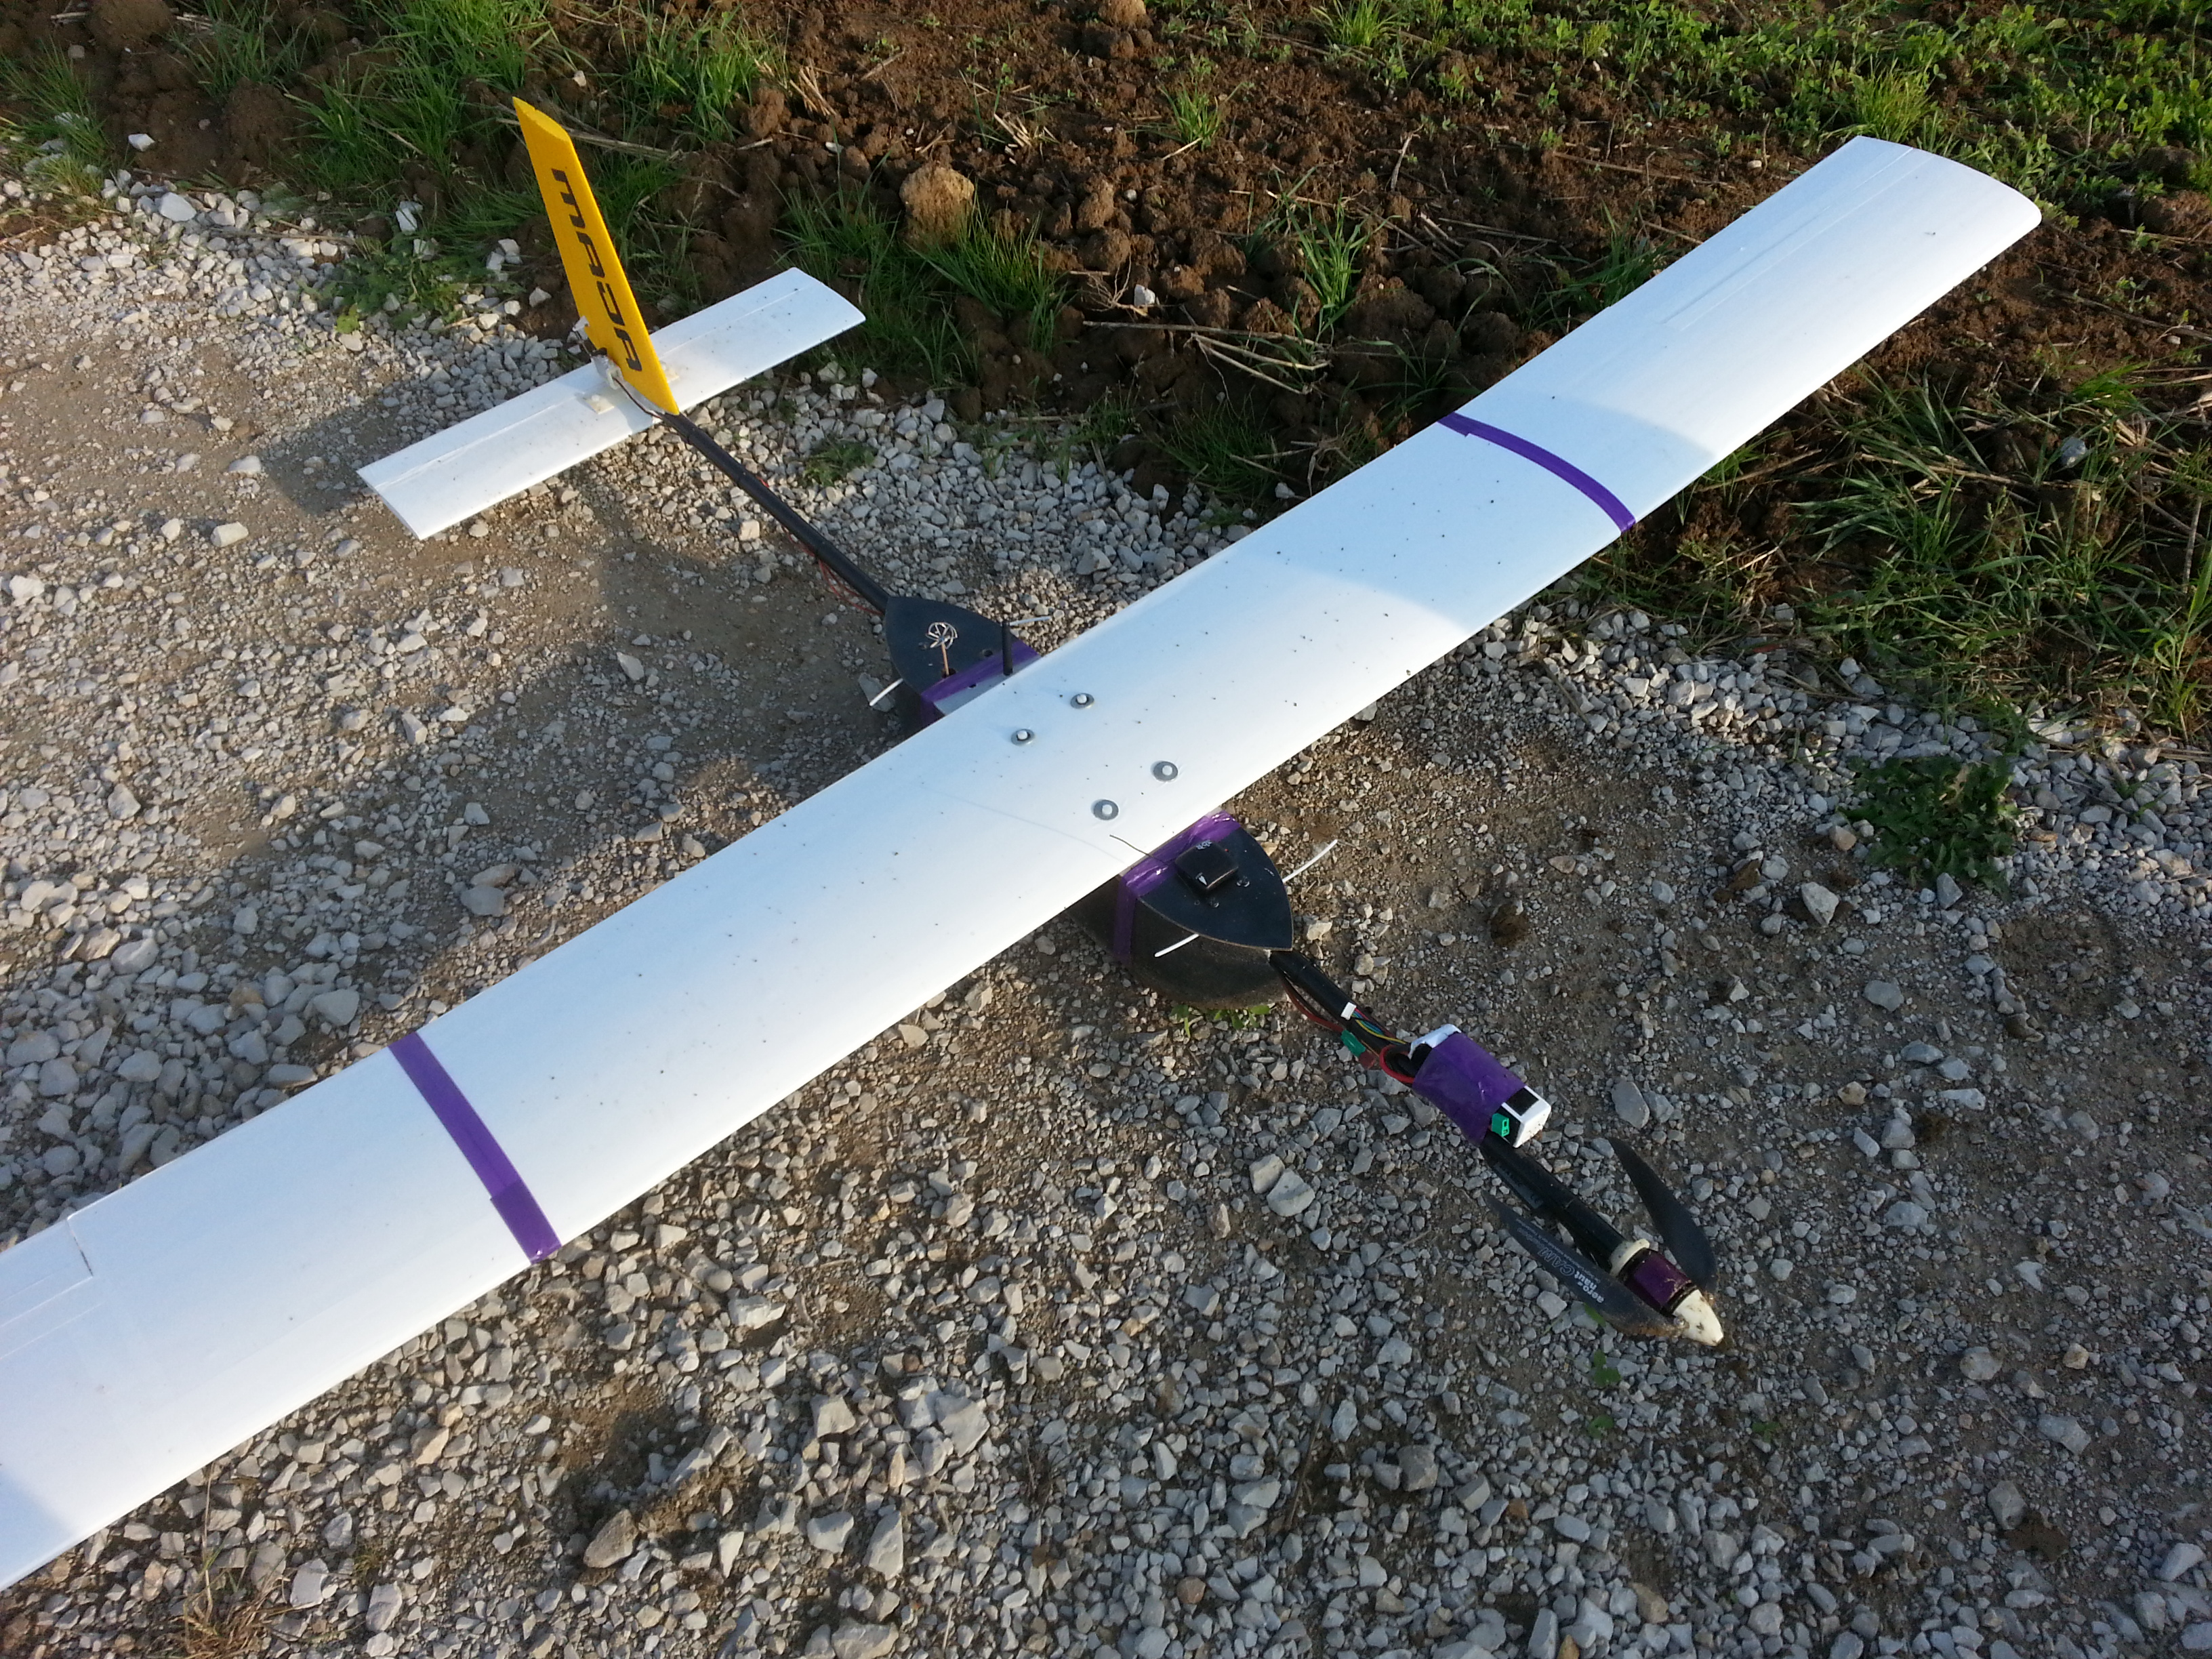
\includegraphics[width=0.9\textwidth]{bilder/Fotos/AUVSI-MAYA-Hybrid.jpg} 
\caption{Frühe Vorversuche für das AUVSI 2015 Flugzeug} 
\label{Frühe Vorversuche für das AUVSI 2015 Flugzeug}
\end{figure}

\begin{figure}[H]
\centering
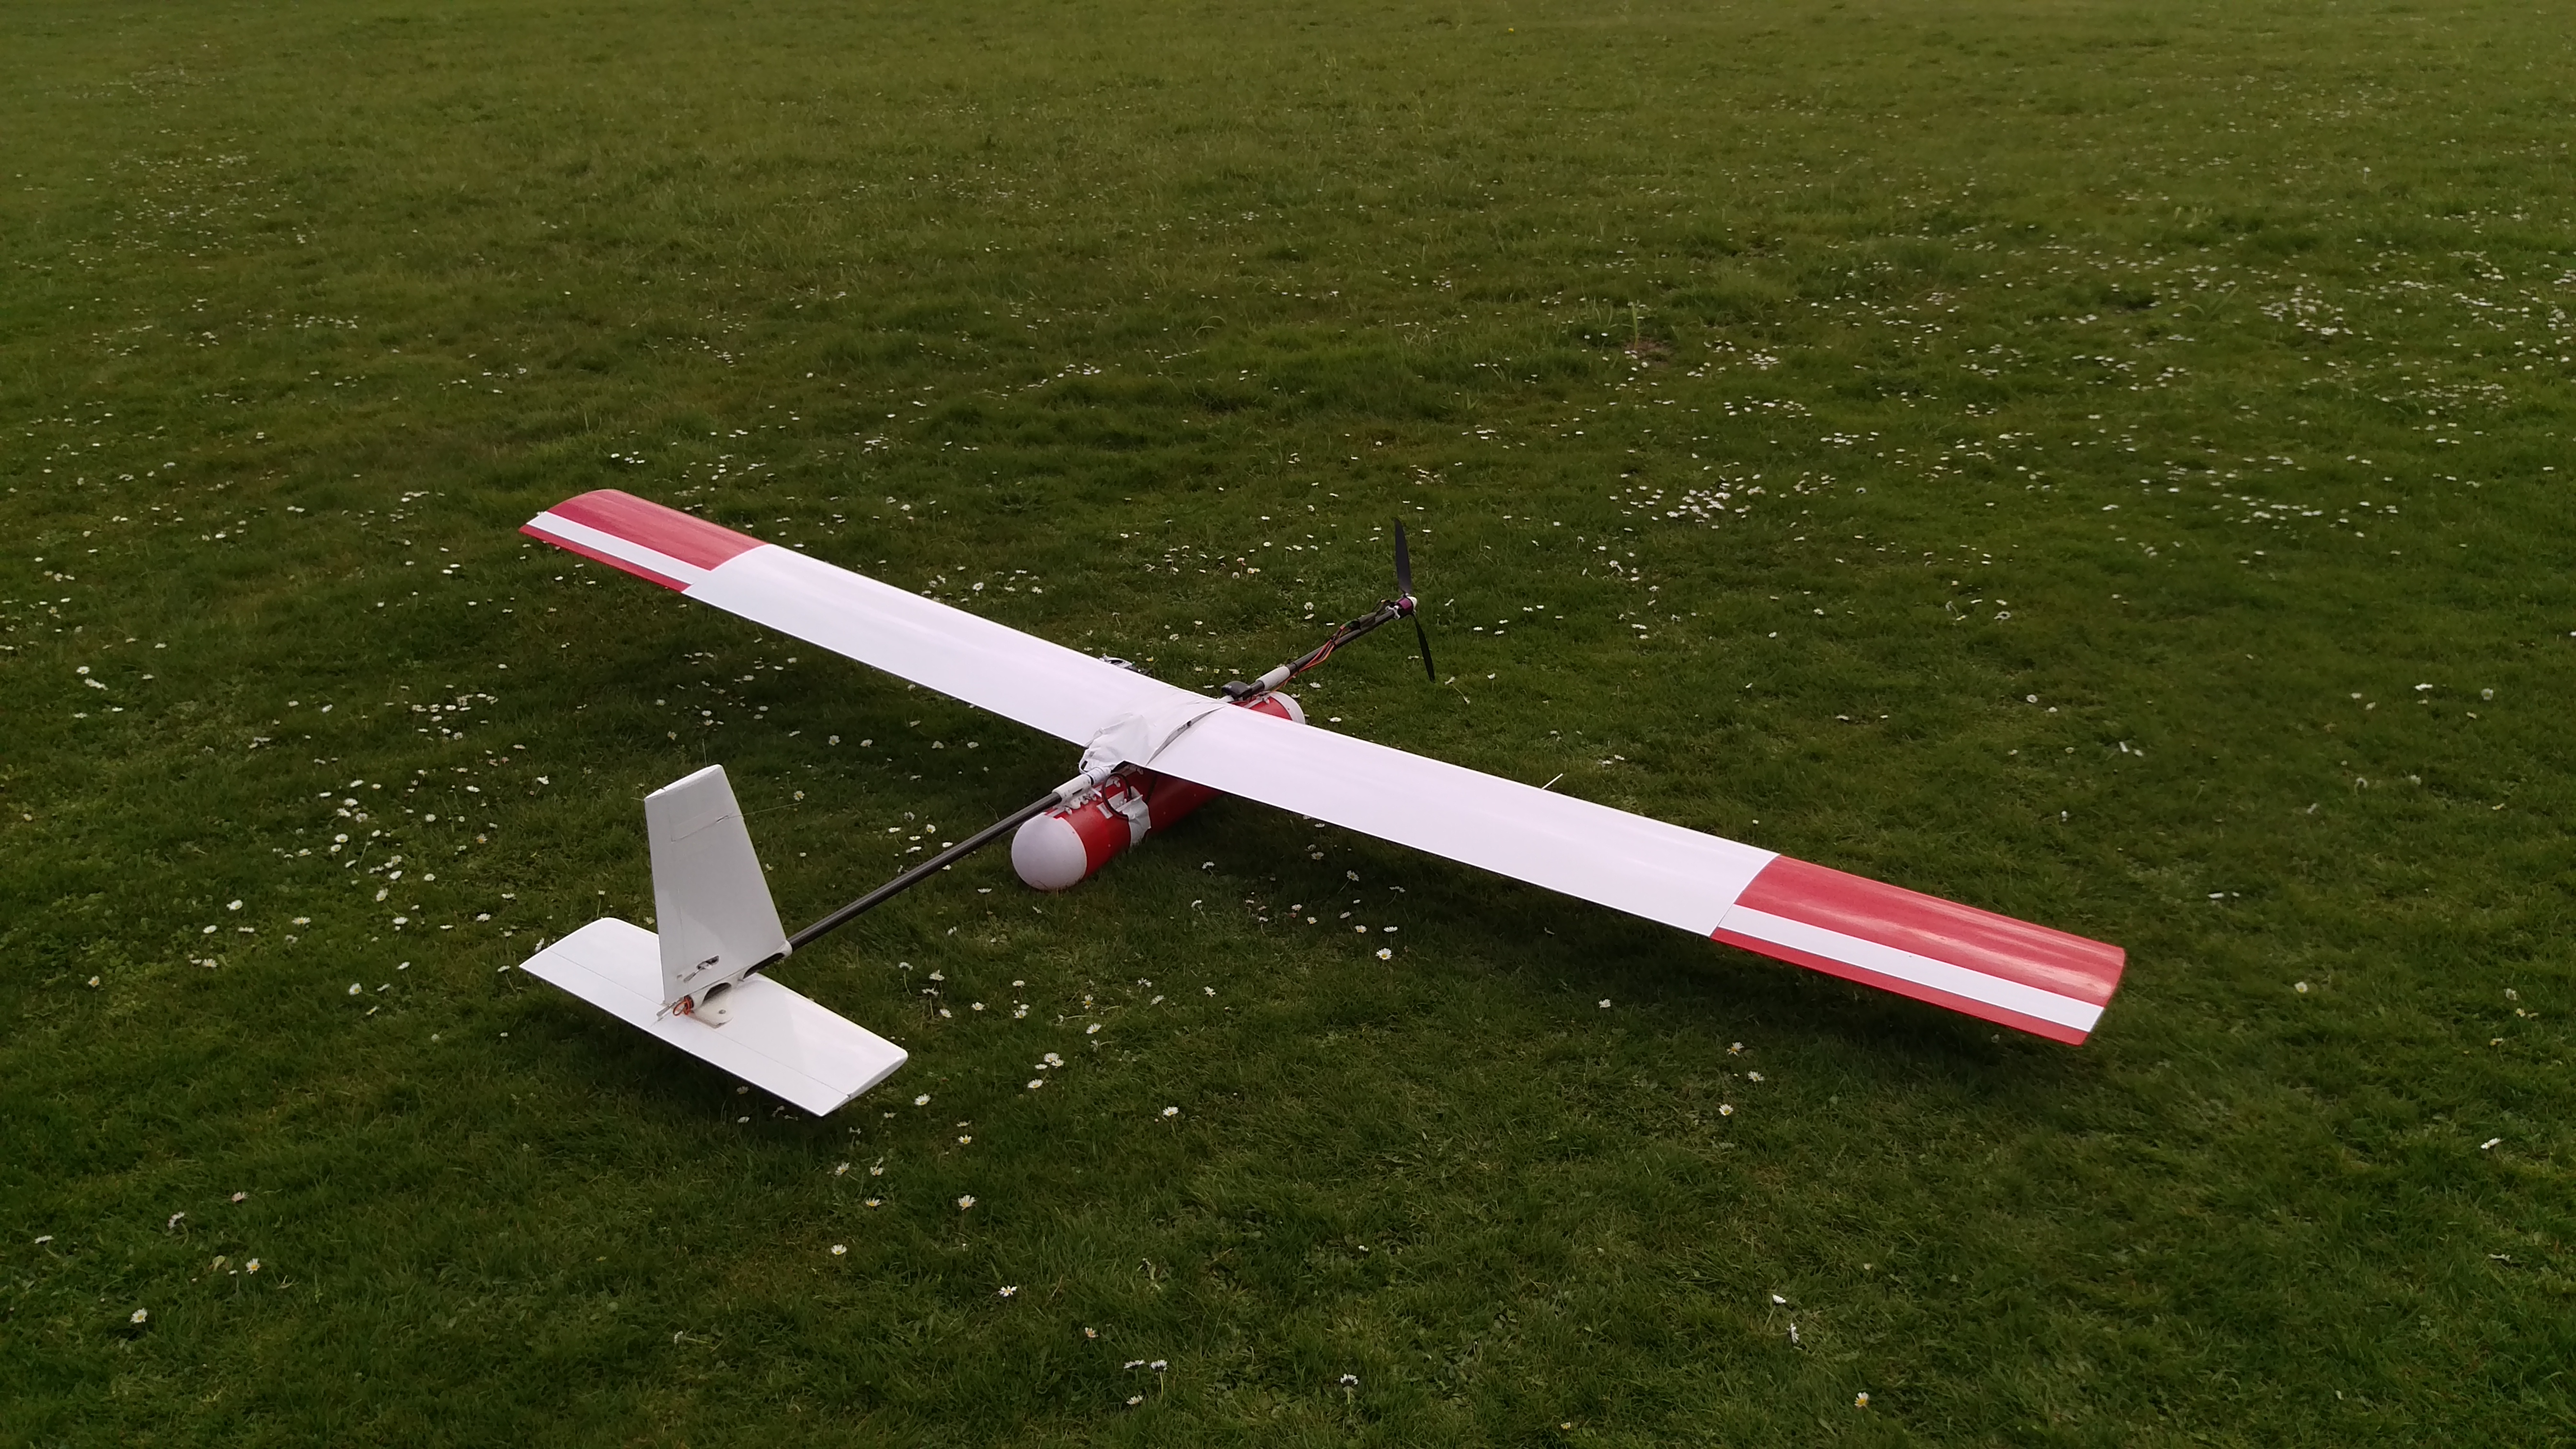
\includegraphics[width=0.9\textwidth]{bilder/Fotos/AUVSI_2015.jpg} 
\caption{Das AUVSI 2015 Modell in Einsatzzustand am Testflugplatz} 
\label{Das AUVSI 2015 Modell in Einsatzzustand am Testflugplatz}
\end{figure}

\begin{figure}[H]
\centering
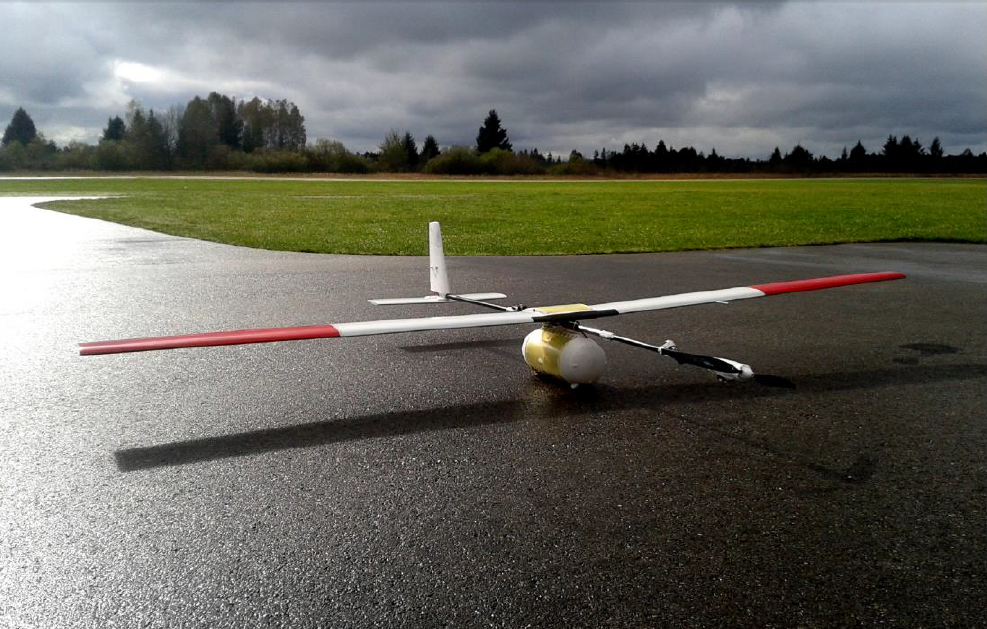
\includegraphics[width=0.9\textwidth]{bilder/Fotos/Ecuadorflieger_Koenigsdorf.png} 
\caption{Für die Fotomission in Ecuador modifizierter AUVSI 2015 Flieger in Königsdorf} 
\label{Für die Fotomission in Ecuador modifizierter AUVSI 2015 Flieger in Königsdorf}
\end{figure}

\begin{figure}[H]
\centering
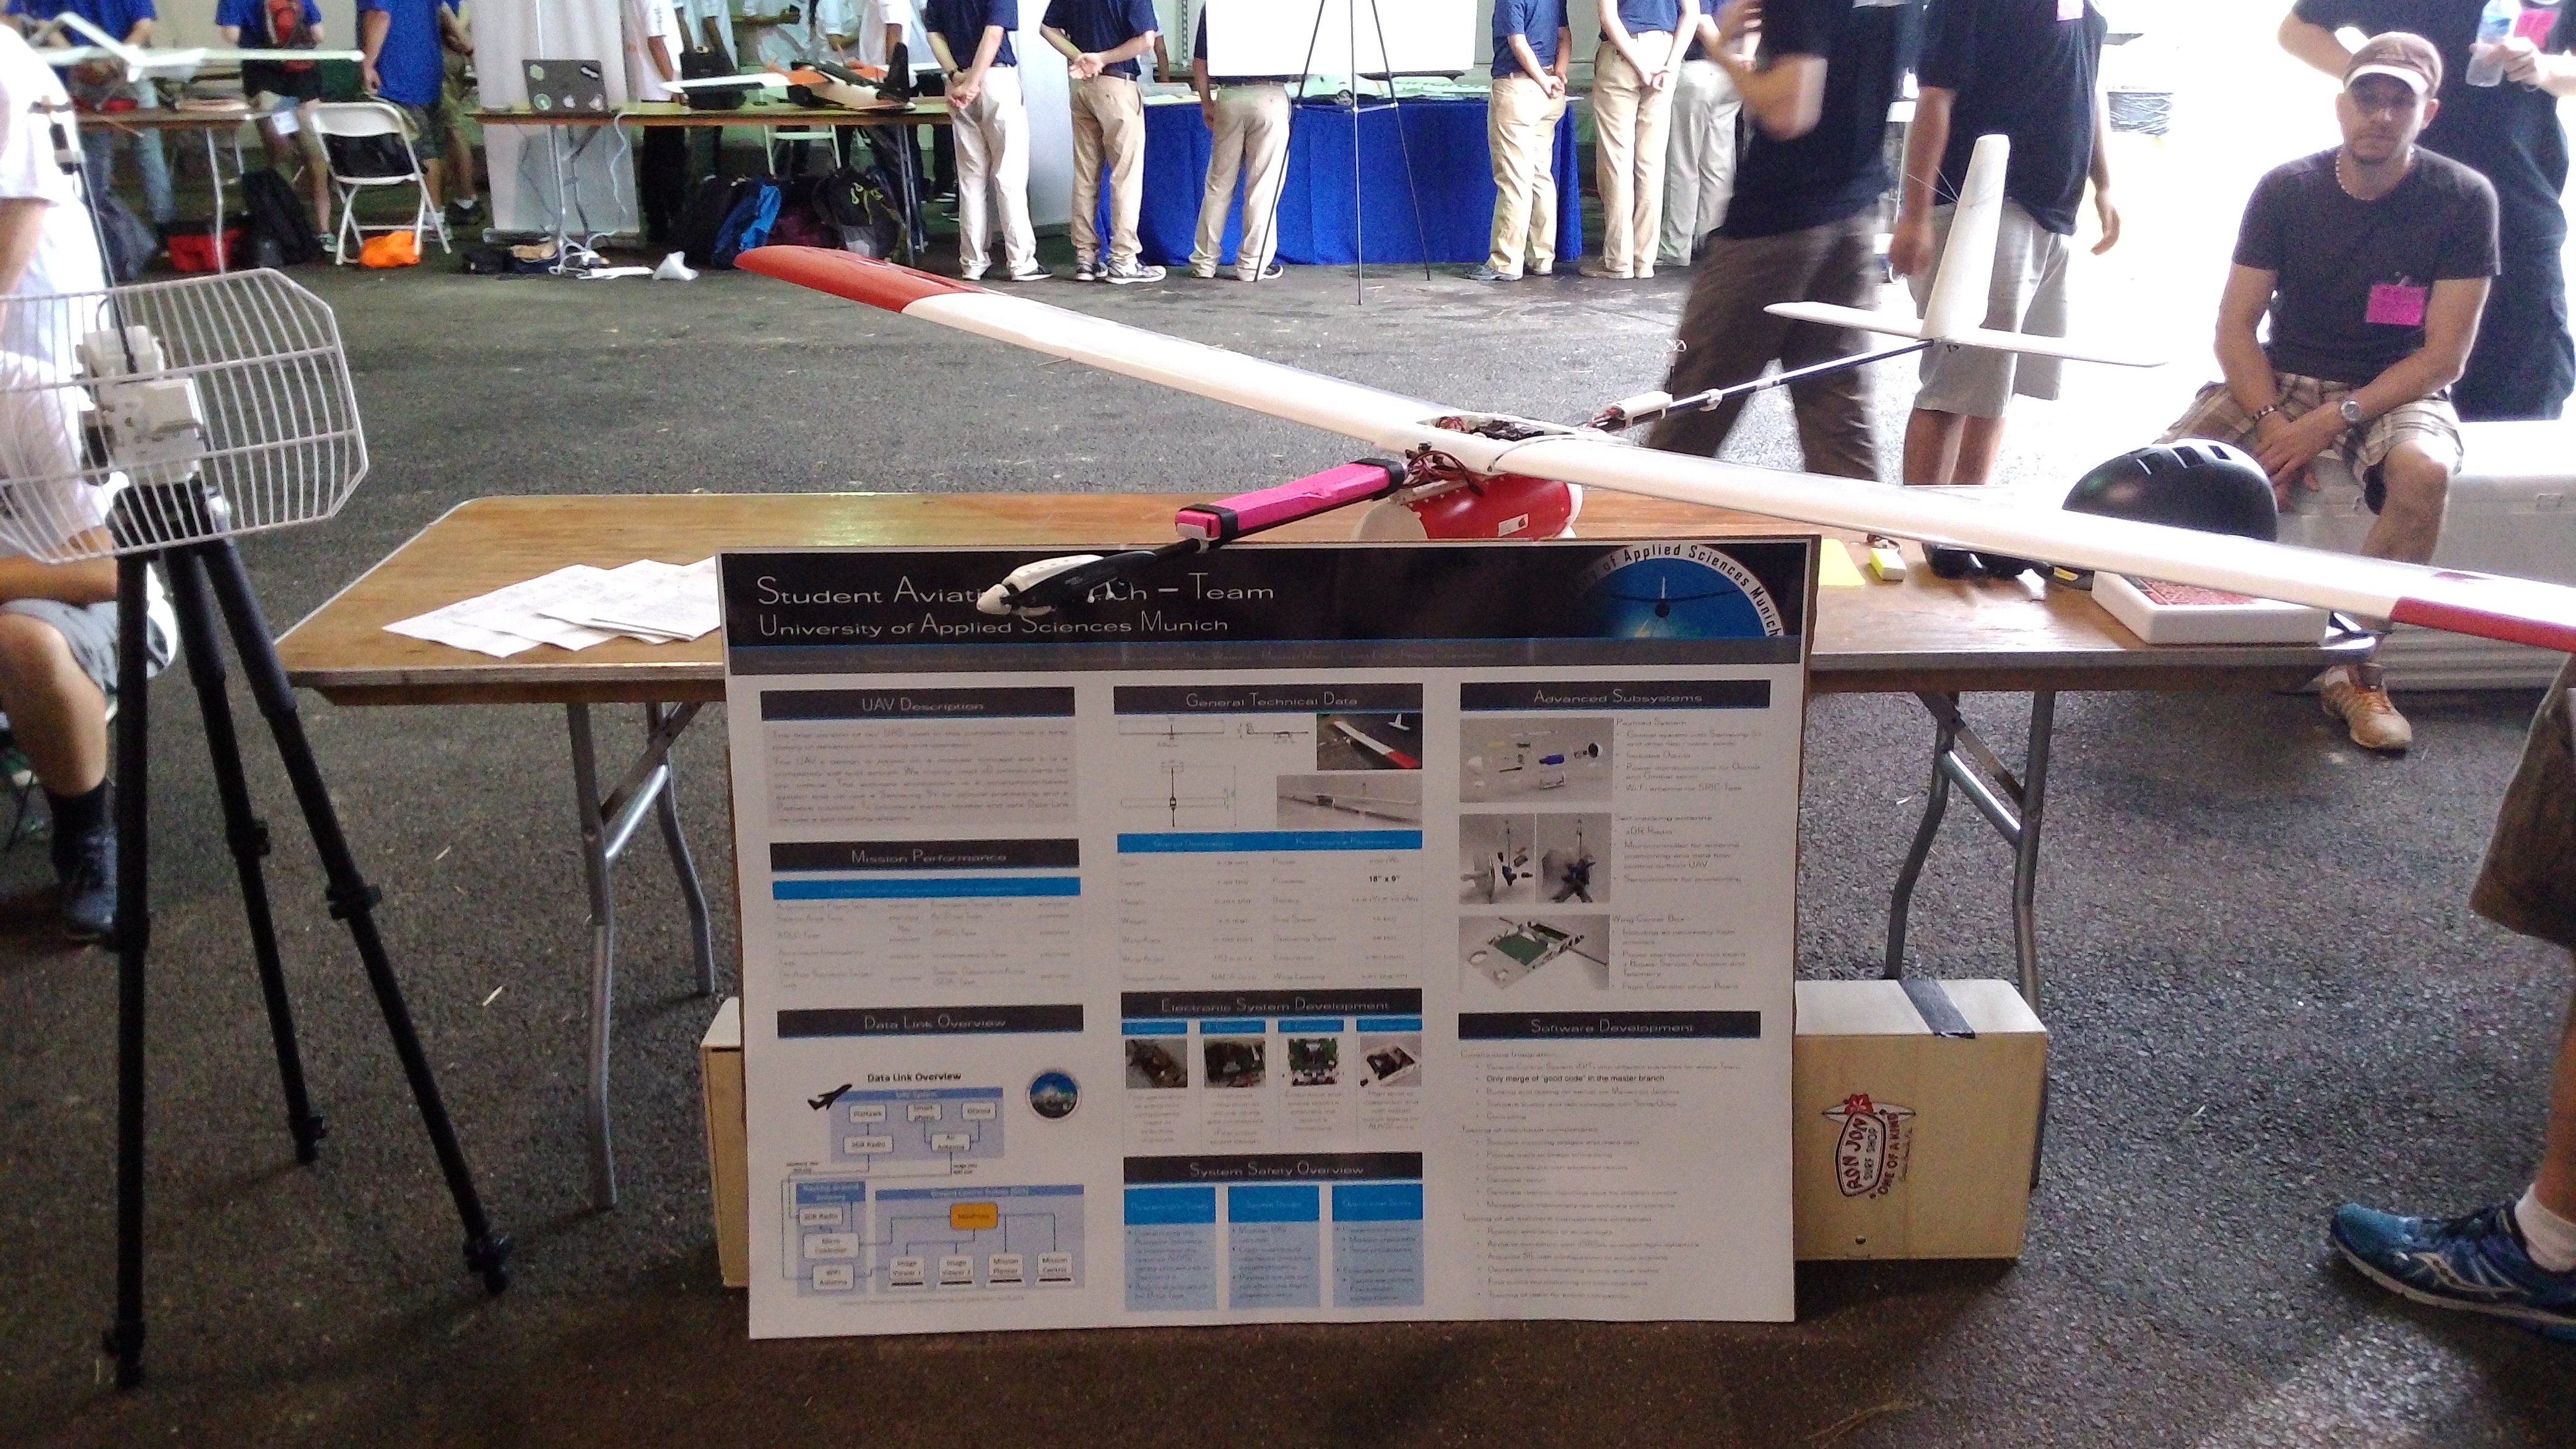
\includegraphics[width=0.9\textwidth]{bilder/Fotos/AUVSI_2016_Display.jpg} 
\caption{Der AUVSI 2016 Flieger beim Display auf dem Wettberwerb} 
\label{Der AUVSI 2016 Flieger beim Display auf dem Wettberwerb}
\end{figure}

\cleardoublepage

\chapter{Anforderungen an die Flugplattform}\label{cha:Anforderungen an die Flugplattform}

\section{Anforderung an das Flugzeug}

\section{Aufgaben der Elektronik}

\section{Anforderung an die Elektronik}

\cleardoublepage

\chapter{Fortschreitende Elektronikentwicklung}\label{cha:Elektronikentwicklung}

In diesem Kapitel der Arbeit wird die Umsetzung der diversen Konzept und Strukturanforderungen in Hardware betrachtet. Dabei werden hier ausgesuchte Beispiele aus mehreren Vergangenen Jahren Vorgestellt und Technisch erläutert.
Dabei wird die kontinuierlich Fortschreitende Implementierung von Erfahrung im Zusammenspiel mit dem Modularen Gesamtkonzept aufgezeigt.

\section{Ursprünglicher Elektronikzustand}

Die in der Saison 2014 begonnen Voruntersuchungen fanden mit dem Flugsystem 'Maya' statt.
Abseits von Strukturellen und Flugmechanischen Problemen war auch die Elektronik eine kontinuierliche Quelle von Fehlern und Ausfällen des Flugzeugs.
Dies war größtenteils auf die Mangelnde Erfahrung im Umgang mit einem System eines solchen Komplexitätgrades zurückzuführen.Aber auch eine noch unzureichende Ausstattung mit Werkzeug,  Testmöglichkeiten und Methoden in Kombination mit der Unübersichtlichen Kabelführung erschwerte die Fehlersuche.
Auch die ersten versuche mit einem selbst gebauten Flächenmodell waren mit ähnlichen Schwierigkeiten in der Elektronik behaftet.

\begin{figure}[H]
\centering
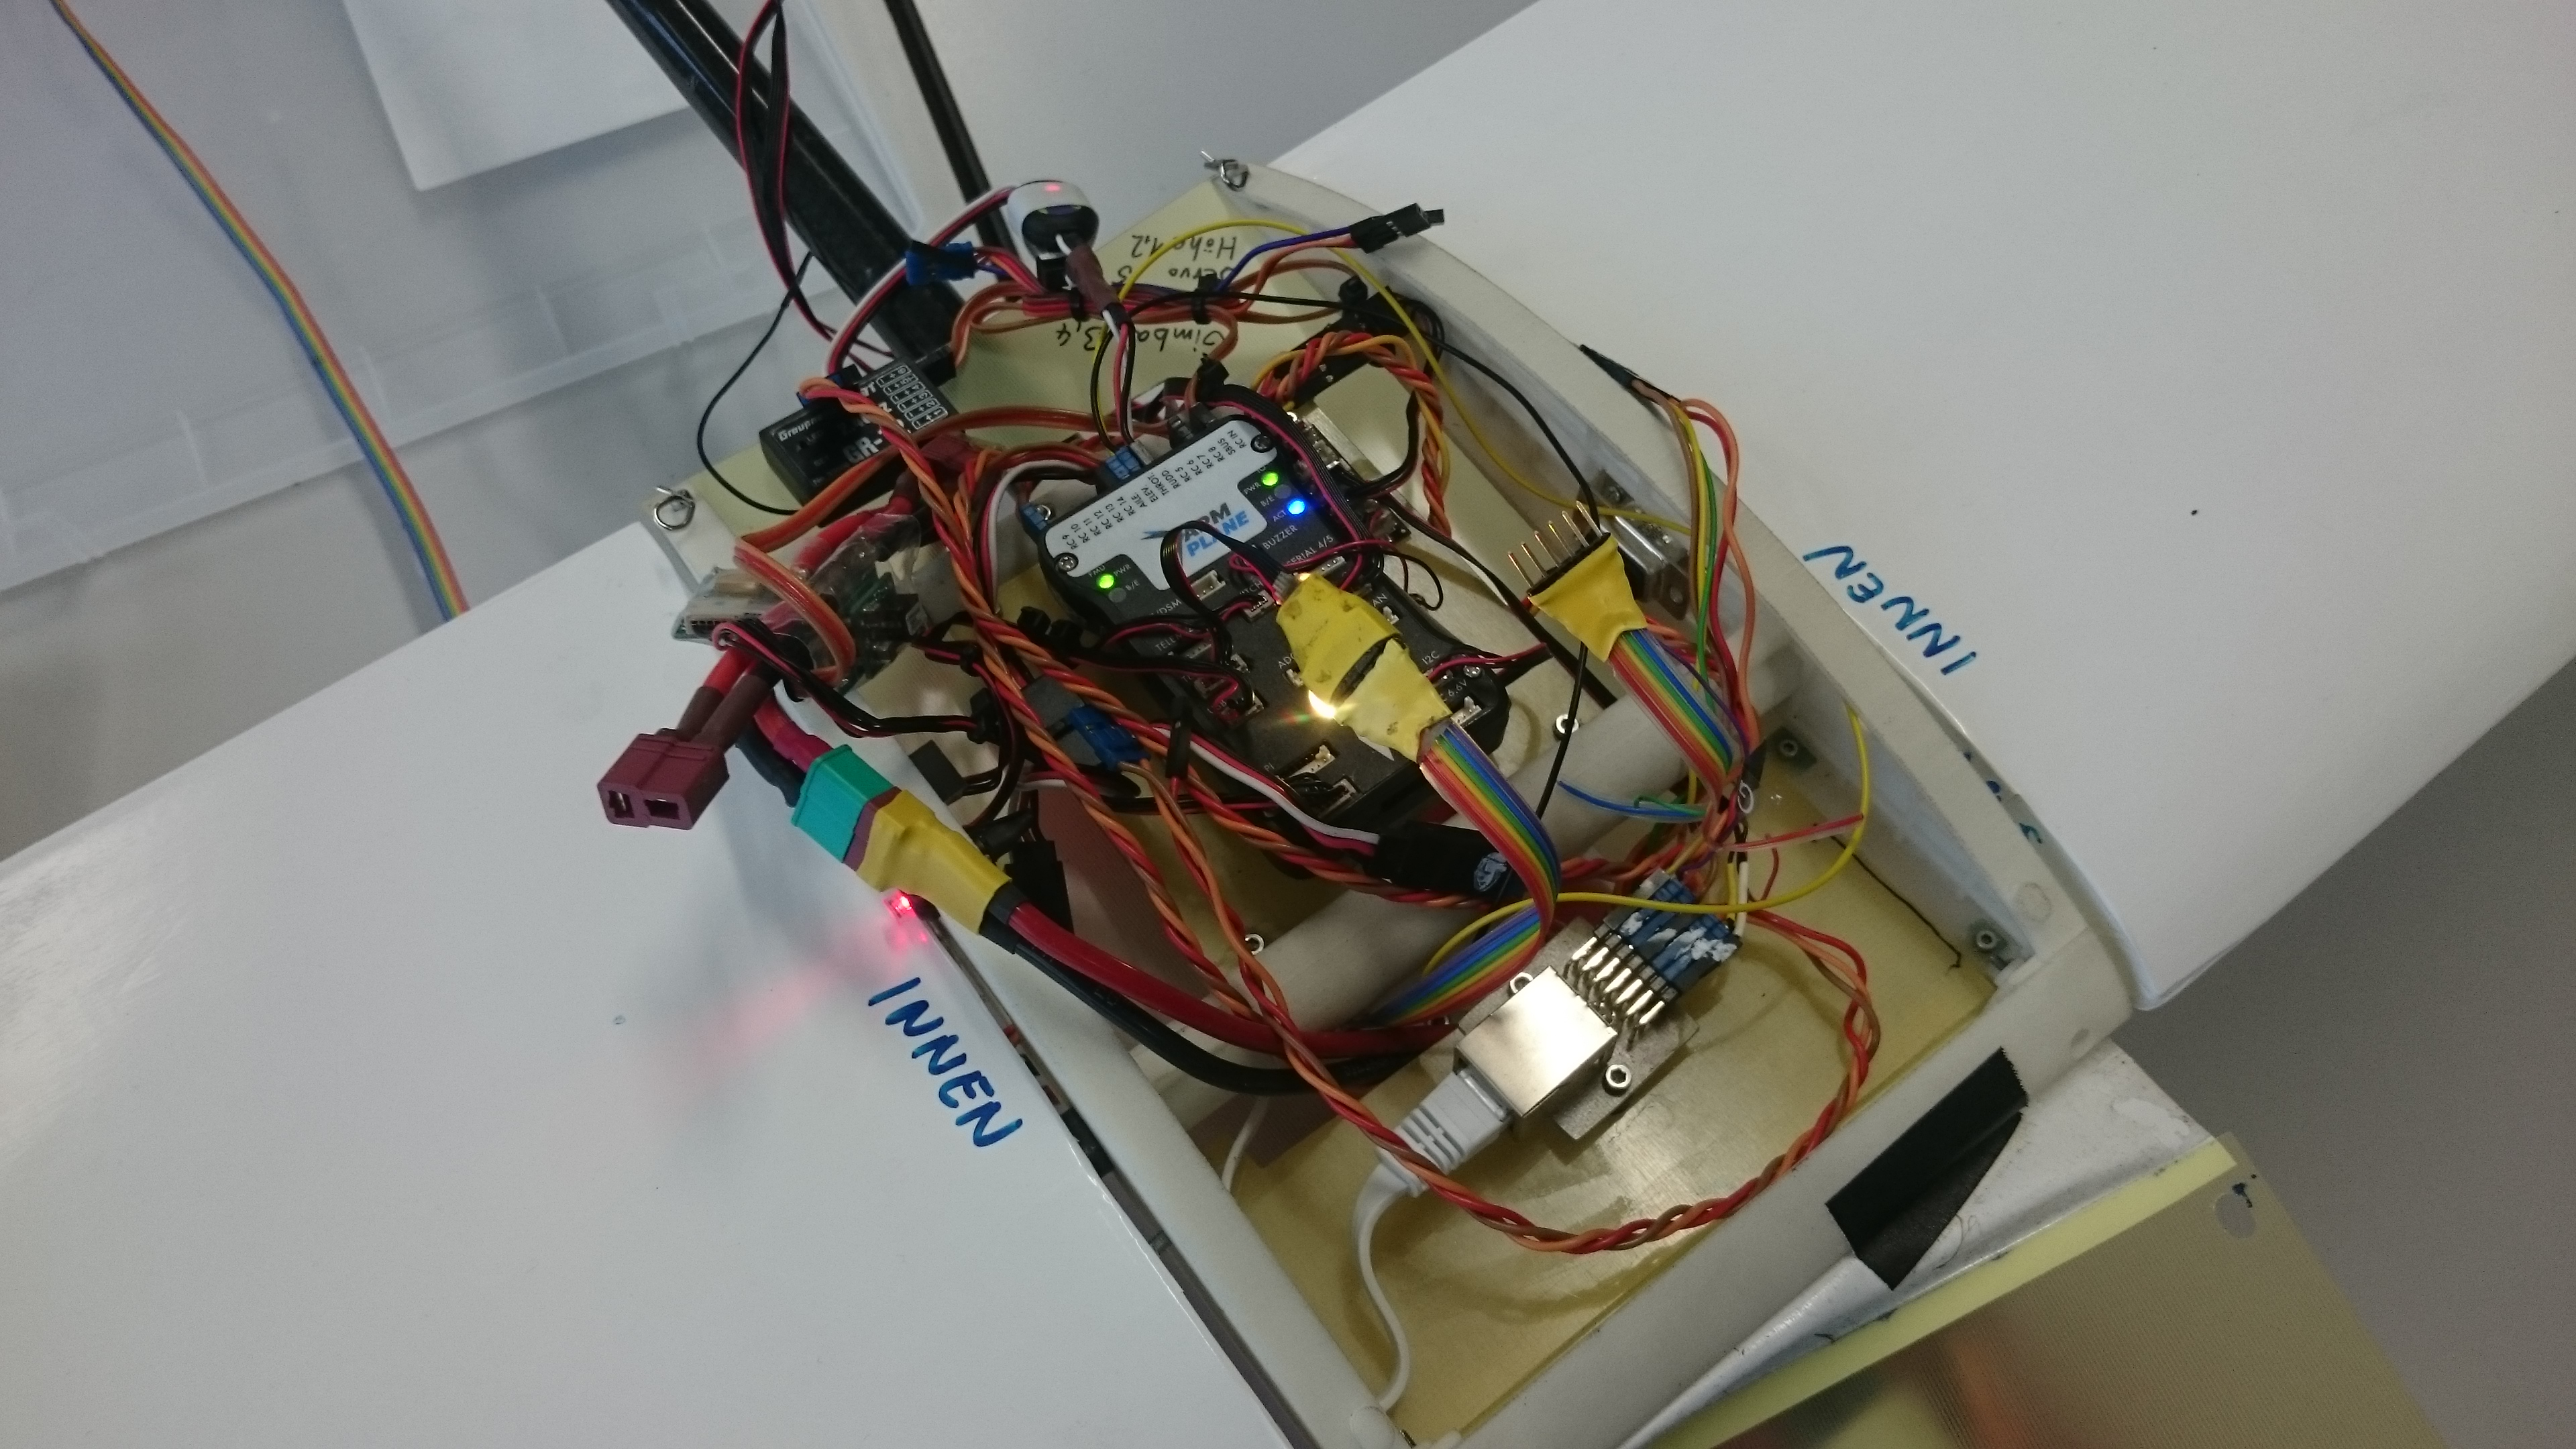
\includegraphics[width=0.9\textwidth]{bilder/Fotos/Elektronik_Kabelsalat_2015.jpg} 
\caption{Anblick der Elektronik zu Beginn 2015} 
\label{Anblick der Elektronik zu Beginn 2015}
\end{figure}

\section{Neue Platinenaufteilung}

Aus diesen Erfahrungen entstand das Eingangs vorgestellte Konzept für die Elektronik des Fliegers.
Dieses Konzept wurde 2015 erstmals angewandt, um eine Übersichtliche und einfach handhabbare Hardwareplattform mit leicht überprüfbaren Funktionen Umzusetzen.

\subsection{Leistungsplatine}

\subsubsection{Schaltplan}

\begin{figure}[H]
\centering
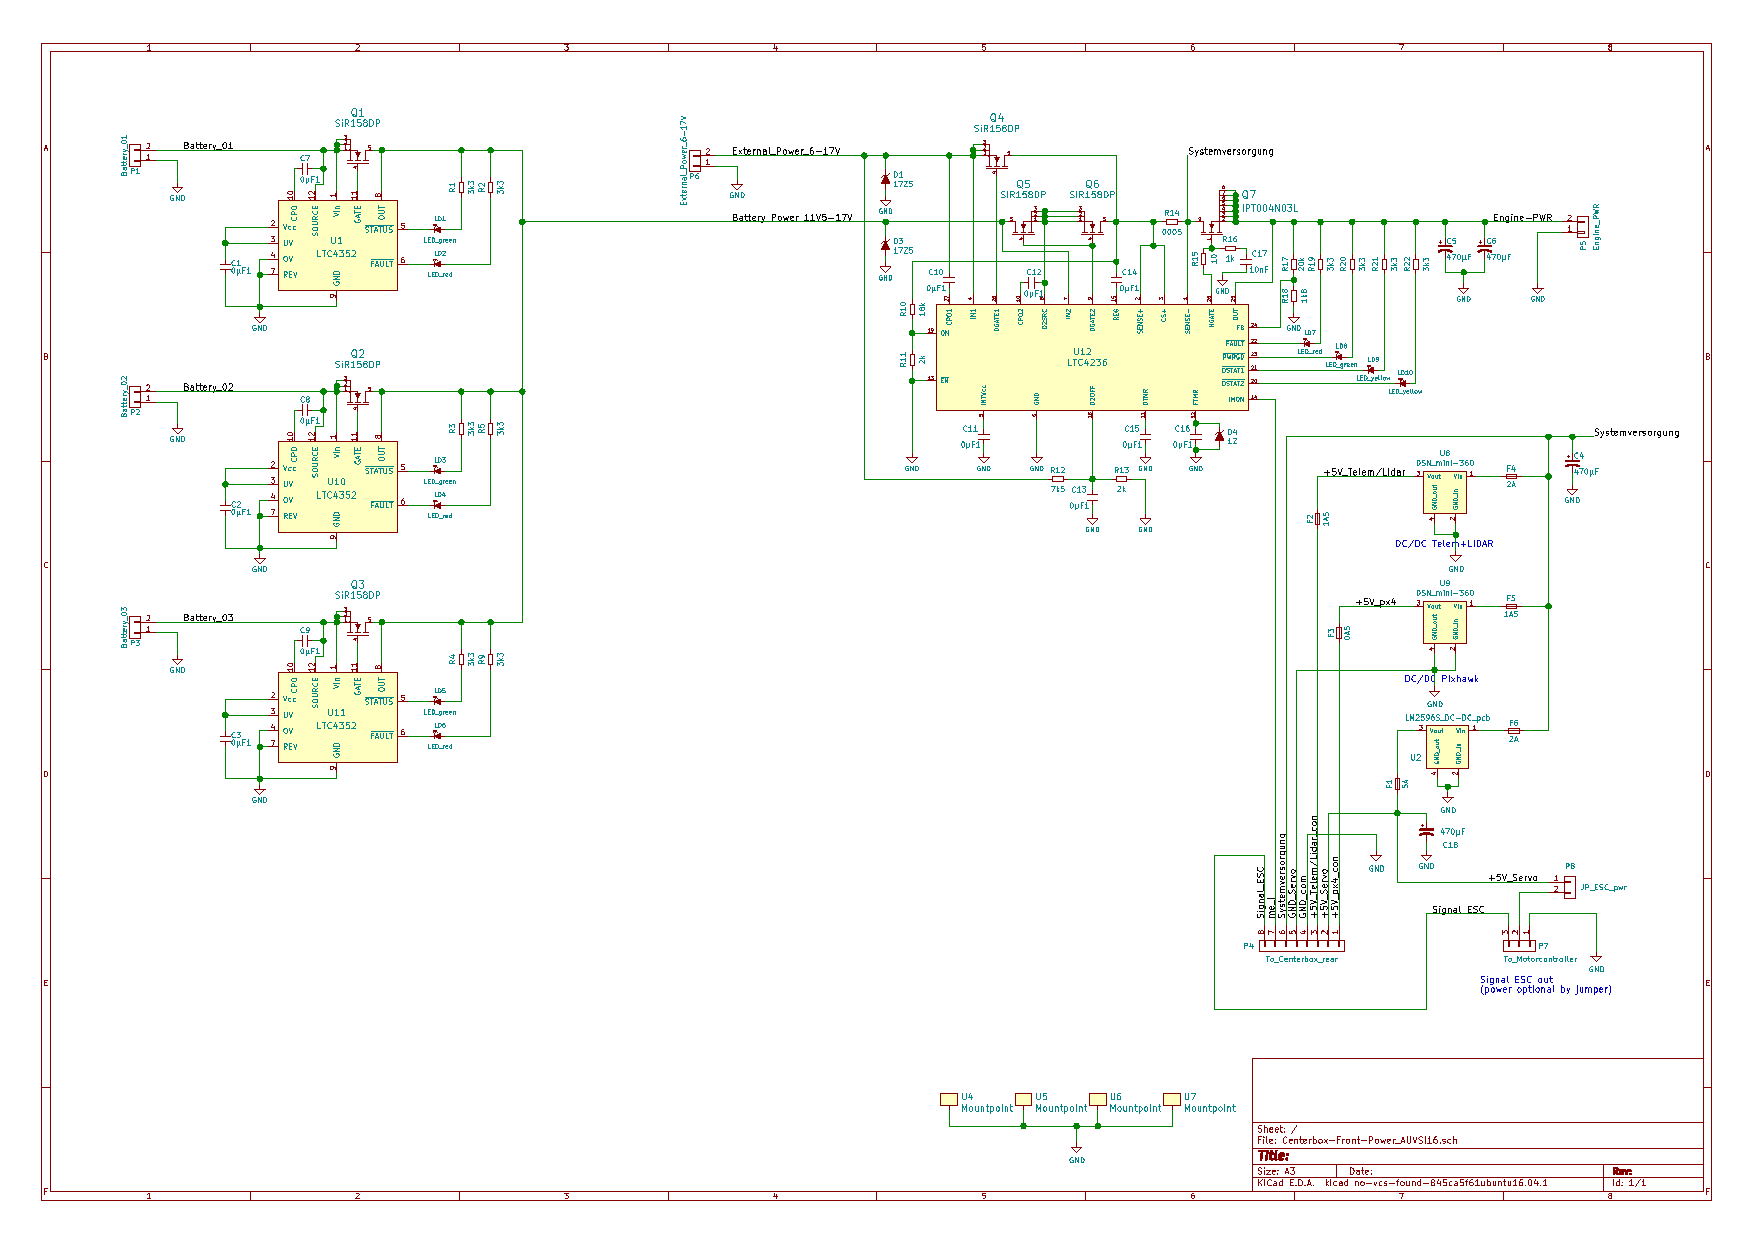
\includegraphics[width=0.9\textwidth]{bilder/Centerbox/Centerbox-Front-Power_AUVSI16.pdf} 
\caption{Schaltplan der Leistungsplatine} 
\label{fig:Schaltplan der Leistungsplatine}
\end{figure}

\subsubsection{Platinenlayout}

\begin{figure}[H]
\centering
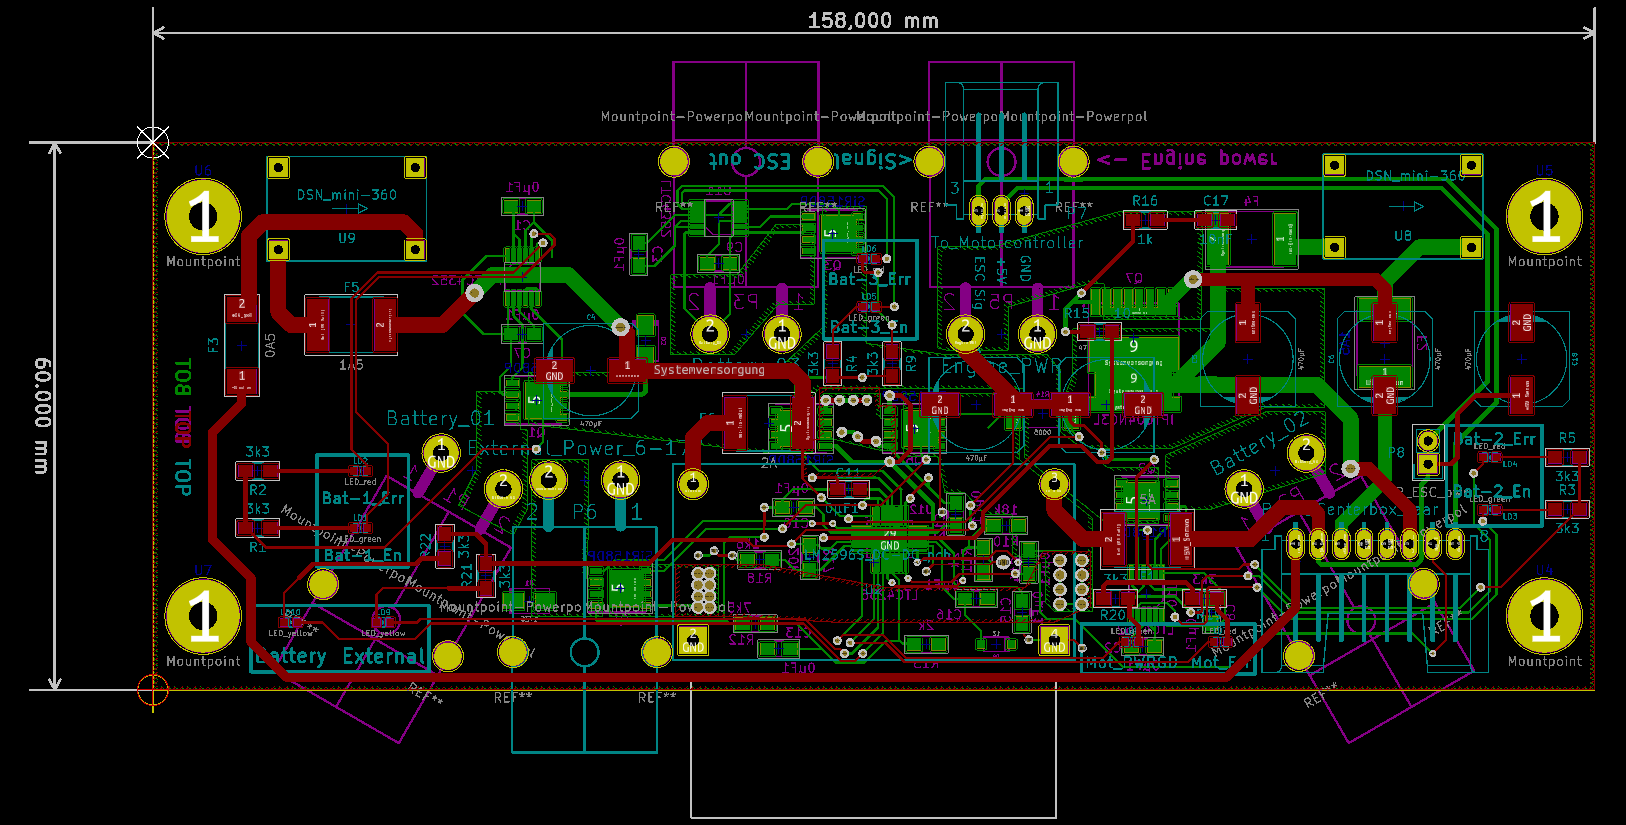
\includegraphics[width=0.9\textwidth]{bilder/Centerbox/Centerbox-Front-Power_AUVSI_2016_rev-01_layout.png} 
\caption{Layout der Leistungsplatine} 
\label{fig:Layout der Leistungsplatine}
\end{figure}


\subsection{Autopilotenplatine}

\subsubsection{Schaltplan}

\begin{figure}[H]
\centering
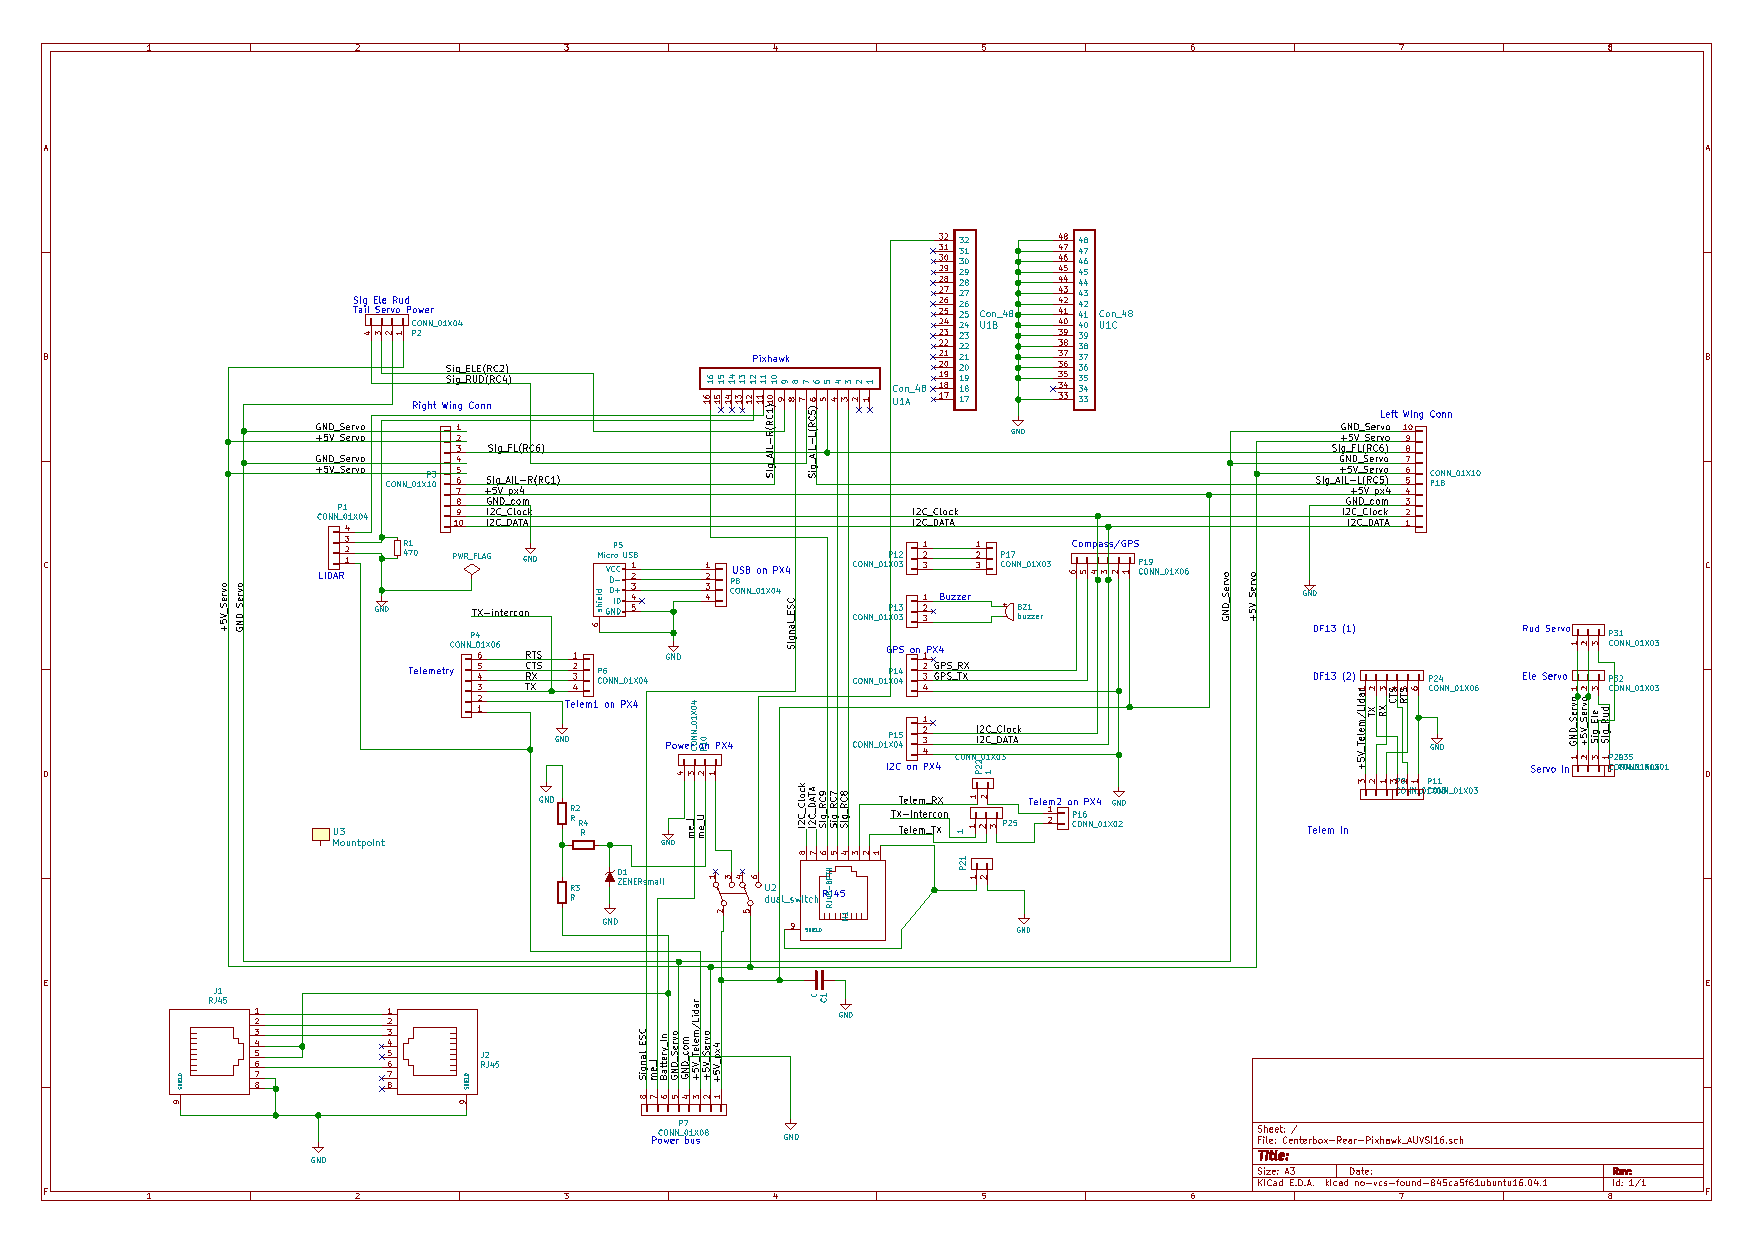
\includegraphics[width=0.9\textwidth]{bilder/Centerbox/Centerbox-Rear-Pixhawk_AUVSI16.pdf} 
\caption{Schaltplan der Autopilotenplatine} 
\label{fig:Schaltplan der Autopilotenplatine}
\end{figure}

\subsubsection{Platinenlayout}

\begin{figure}[H]
\centering
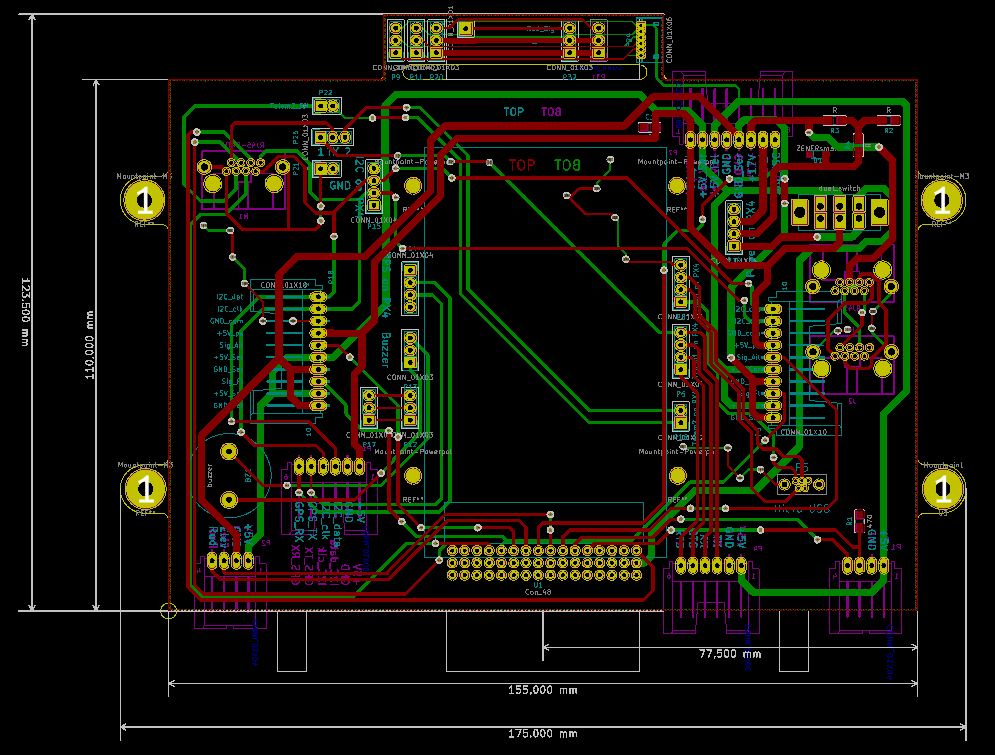
\includegraphics[width=0.9\textwidth]{bilder/Centerbox/Centerbox-Rear-Pixhawk_AUVSI_2016_rev-01-layout.png} 
\caption{Layout der Autopilotenplatine} 
\label{fig:Layout der Autopilotenplatine}
\end{figure}

\section{Bedien- und Schutz Konzepte}

\subsection{Eineindeutige Verbinderauswahl}

Für die angepasste Führung von Leistungspfaden und Signalpfaden wurden im Laufe des bisherigen Projekts je zwei verschiedene Steckersysteme eingesetzt.
Die Leistungsverbinder sind lediglich in Plus und Minuspol aufgeteilt und die Korrekte Montage wird über eine Mechanische Kodierung sichergestellt.
Bei den Signalverbindern wird eine mechanische Kodierung über eine einmalige Anzahl an Kontakten angestrebt.So kann in Verbindung mit der konsequenten Beschriftung aller Gegenstellen auf der Platinenseite eine fehlerhafte Montage quasi ausgeschlossen werden. Dabei werden zum teil auch bewusst Steckverbinder mit mehr Kontakten als zu übertragenden signalen ausgewählt um diese Einendeutikeit zu erreichen.

Die Hochstromverbindungen werden stets mit Kabelquerschnitten von 1,5 mm ausgeführt. Der Mantel besteht aus PVC außer in der Nähe von heißen Bauteilen an denen Silikon zum einsatz kommt.
Zu beginn wurden als Hochstromstecker Bauteile des Typs XT60 der Firma hexTronik verwendet.
Diese werden von den meisten Zukaufbaugruppen der Pixhawk Systems verwendet und ermöglichten eine mechanisch kodierte eindeutige Verbindung.
Sie sind für Ströme von 60 Ampere und Spannungen von 120 V freigegeben.
Jeoch waren diese Steckverbinder nur zur Lötmontage vorgesehen. Es wurde die Erfahrung gemacht das die Verbindungen zur Kabelseite immer wieder versagten. Teils wegen Qualitativ ungenügender Lötstellen, teils wegen Brüchen durch Handhabung mit Bewegung des Kabels am Übergang von der Lötstelle zum Kupferkabel am Steifigkeitssprung.

-->> Bild von XT60 und Powepol 55 

Daraufhin wurde ein neues System mit Crimpmontage gesucht.
Hierfür wurde das System POWERPOLE 45 der Firma Anderson Power Products ausgewählt. Die Steckverbinder sind bis zu einem Dauerstrom von 55 Ampere und einer Spannung von 300 V freigegeben.
Die Kabelbrüche wurden mit dem Ersatz der Lötverbidungen durch das Crimpsystem beseitigt. Sie können in den Quadratischen Gehäusen beliebig nebeneinander eingeclipt werden was größere Steckblöcke ermöglicht. Jedoch führte diese variable Montierbarkeit auch immer wieder zu wiedersprüchlicher Montage von Ladekabeln und Akkus bezüglich der Polposition.
Außer einer klaren Standardisierung der Polung wurde bisher noch keine Konzept gefunden Bedienfehler auszuschließen. 

Beide Systeme verwenden das Prinzip des Kraftschlusses für die Fixierung der Steckverbindung. Die für Montage und Demontage nötigen Kräfte sind jedoch an beengten Stellen im Flieger immer wieder hinderlich bei der Handhabung. Deshalb wird eine Formschlussbasierte Fixierung ähnlich den Signal Steckverbindern erwogen.


Für die Verbindung von Signalleitungen  und Versorgungsleitungen mit kleinen Strömen wurde zu Beginn das Stecksystem MSF der Firma Lumberg verwendet.
Dieses ist für 5 A je Pin bei bis zu 160 V freigegeben. Die Fixierung der Verbindung erfolgt hier über Formschluss in Form einer Lasche im Platinensockel des Verbinders welcher eine Nase am Stecker blockiert. Darüber hinaus besteht noch eine gewisser Kraftschluss über die Kontakte der bei der Demontage der Verbindung oft als unerwünscht hoch eingestuft wurde.


Als Alternative wurden die Verbinder aus der PA Reihe der Firma JST erprobt und mittlerweile in den Einsatz überführt.
Die Stecker sind für 3 A je Pin bei maximal 250 V freigegeben.
Die Fixierung wird auch hier über Formschluss in Gestalt einer Hakennase am Kabelseitigen Stecker realisiert.
Die Verbinder haben sich bisher bewährt, da sie einen guten Kompromiss aus kompakterer Baugröße und guter Handhabung in Montage und Demontage gegenüber den bisher verwendeten MSF Verbindern darstellen.
Die Reduzierte Strombelastbarkeit stellt in der Praxis keinen Nachteil dar.Die Logiksignale bringen nur Ströme im mA Bereich auf und auch die Servoversorgung leitet maximal 1 A.

\begin{figure}[H]

\begin{subfigure}{}
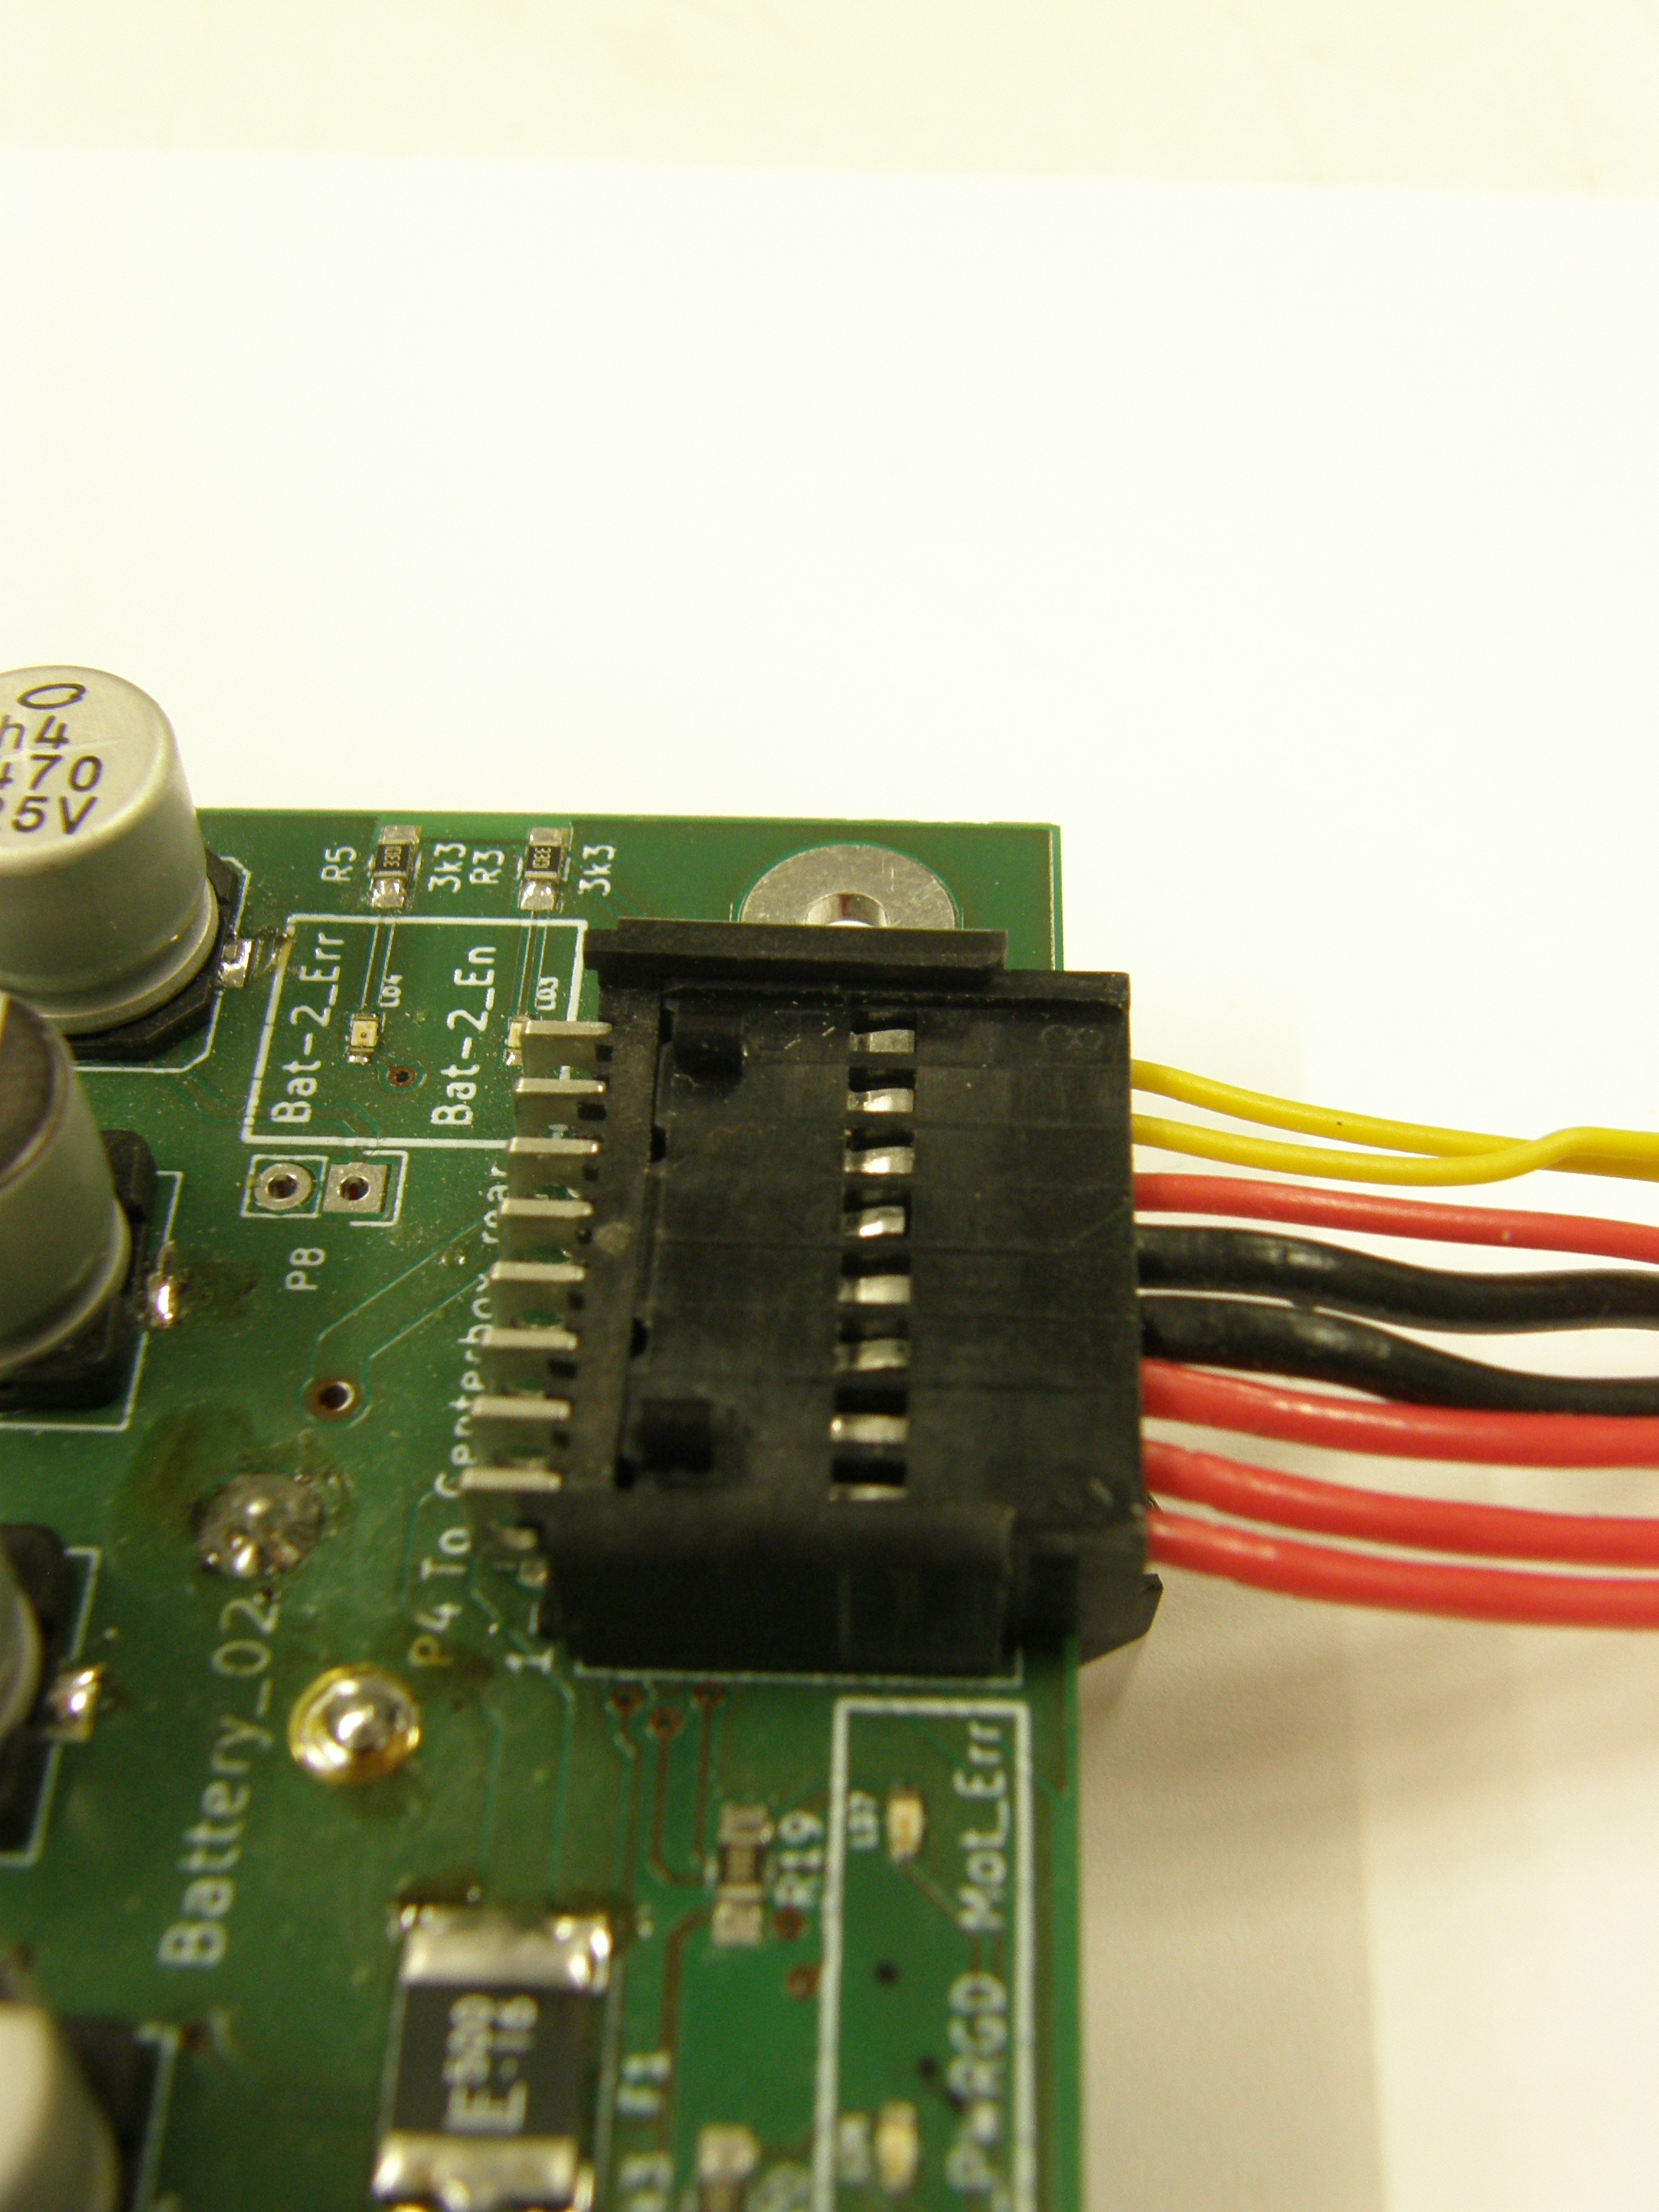
\includegraphics[width=0.6\textwidth, center]{bilder/Stecker/Stecker_Lumberg_MSF.jpg} 
\caption{Der ursprünglich eingesetzte Lumberg MSF Steckverbinder} 
\label{fig:Der ursprünglich eingesetzte Lumberg MSF Steckverbinder}
\end{subfigure}

\begin{subfigure}{}
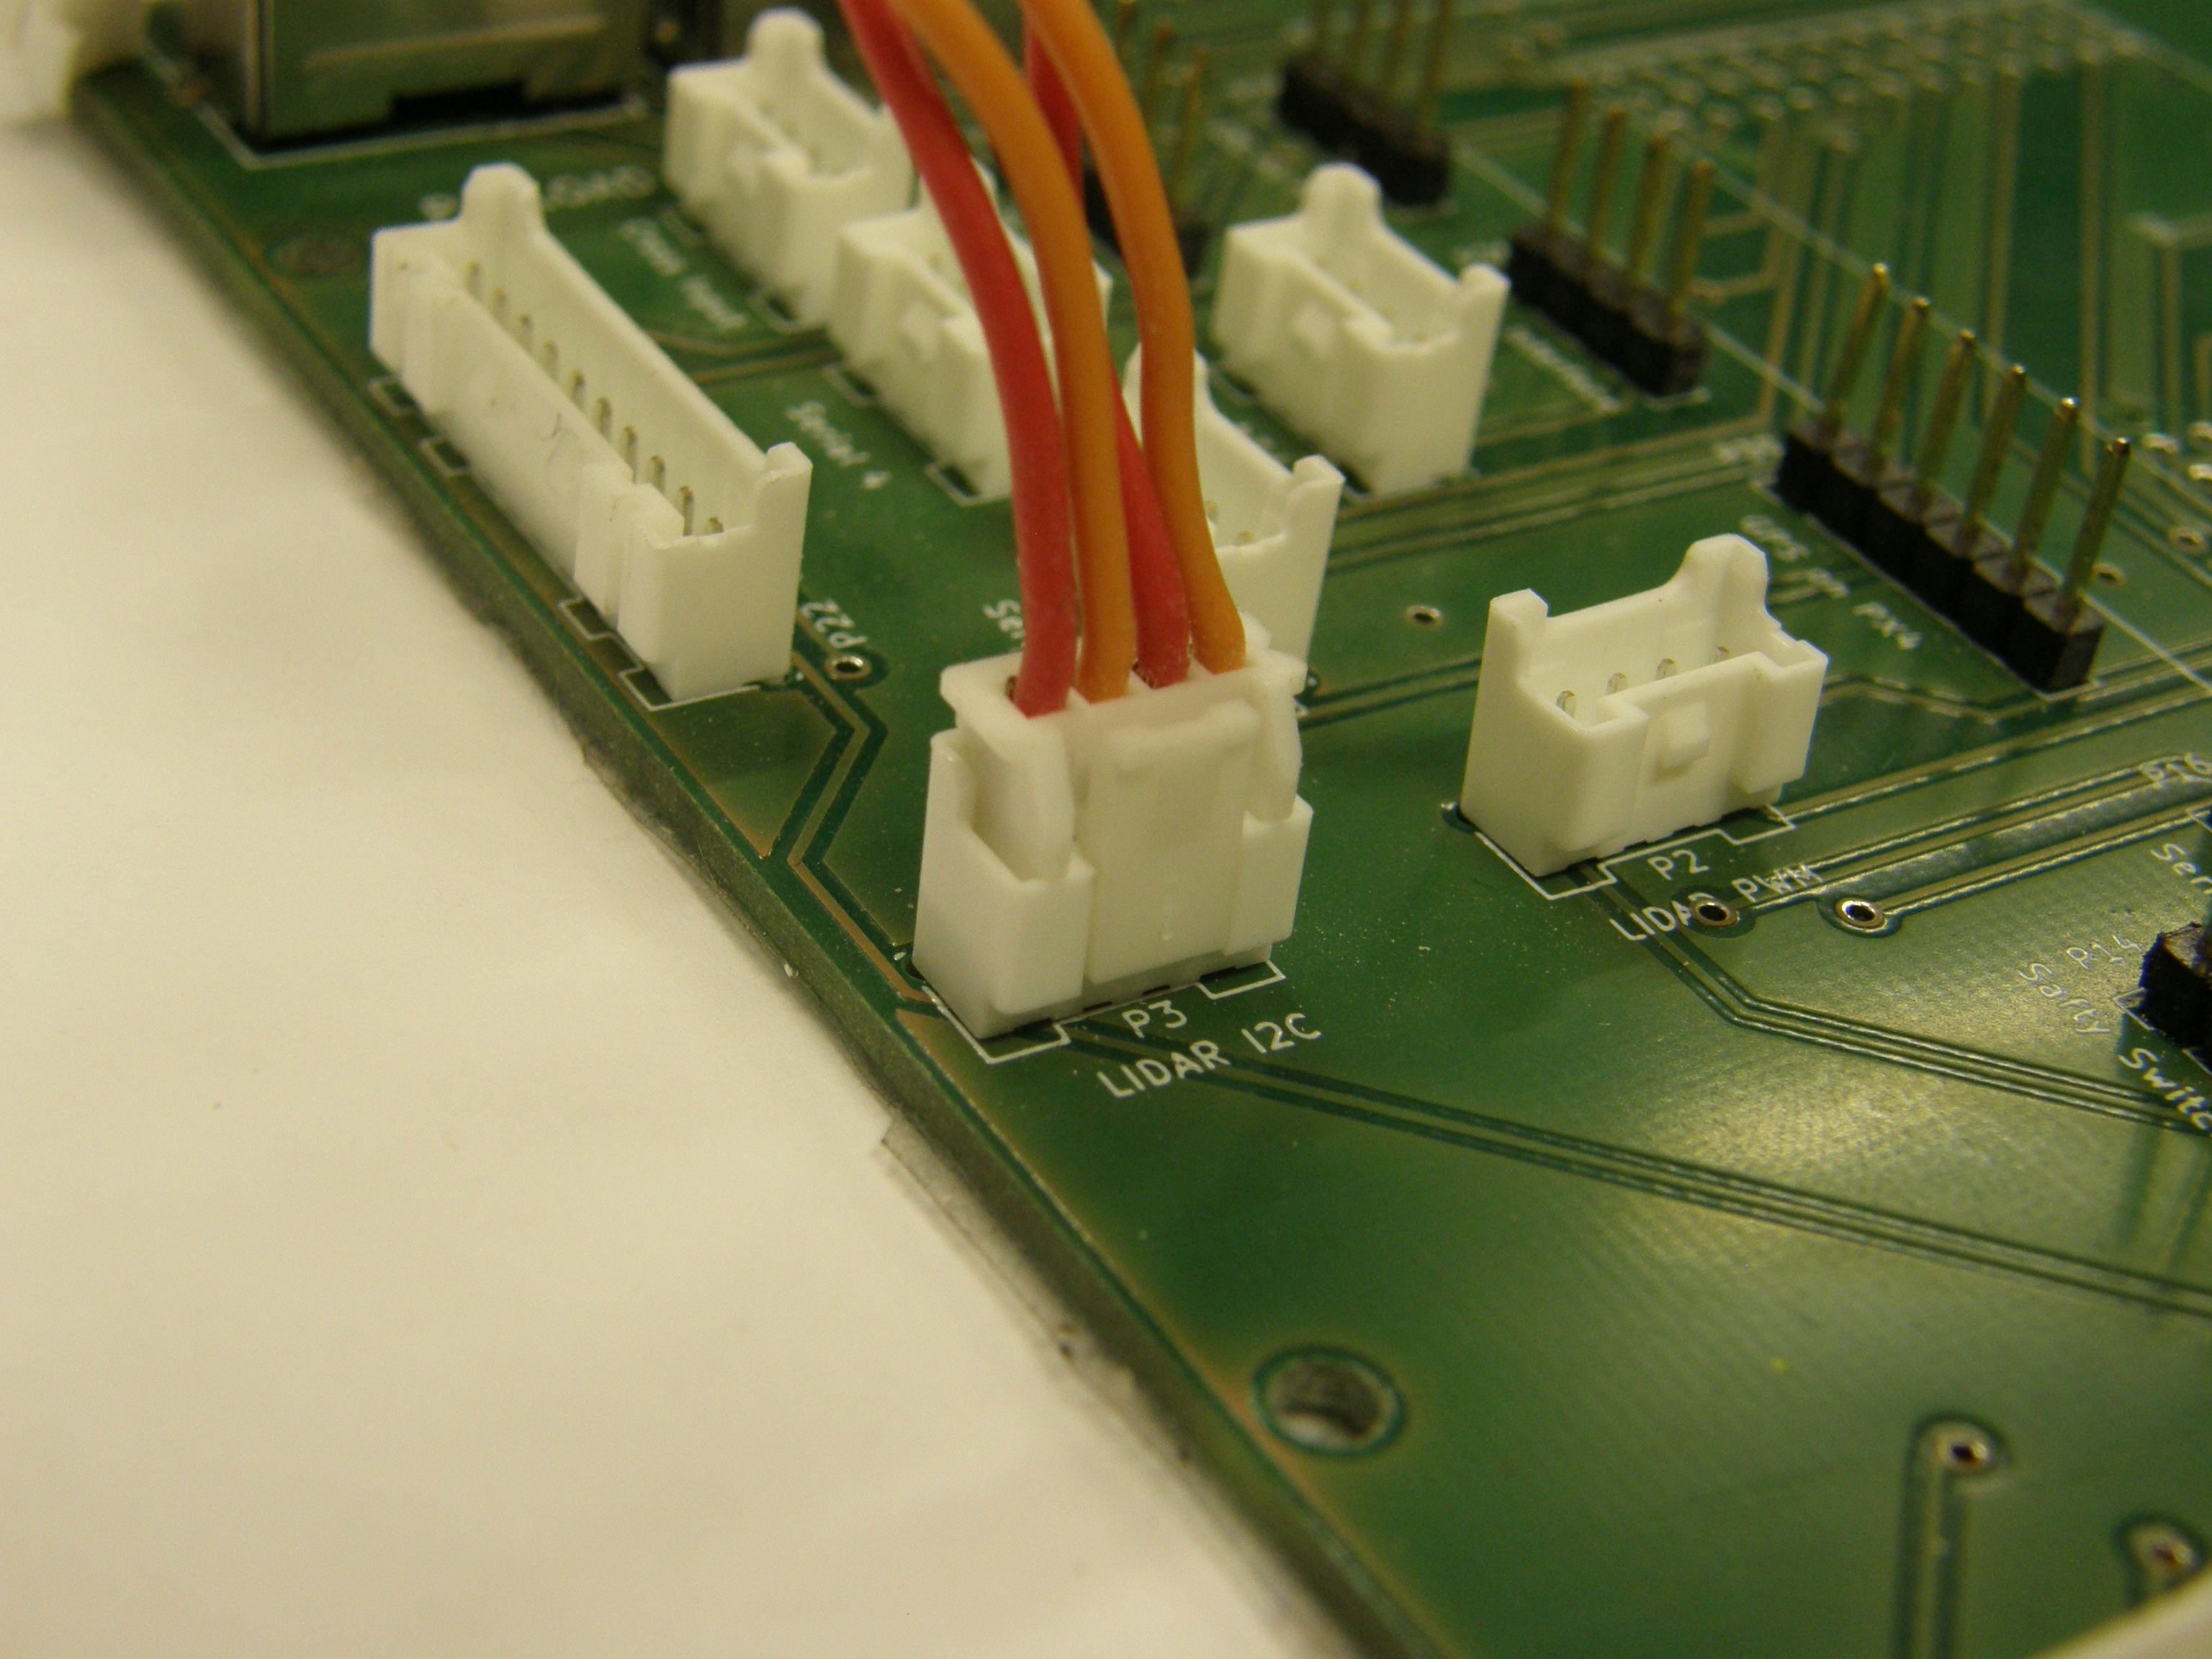
\includegraphics[width=0.6\textwidth, center]{bilder/Stecker/Stecker_JST_PA.jpg} 
\caption{Der mittlerweile eingesetzte JST PA Steckverbinder} 
\label{fig:Der mittlerweile eingesetzte JST PA Steckverbinder}
\end{subfigure}

\end{figure}

Generell soll weiter ein Standardisierung der Verbinder erfolgen und Vollständig eine Fixierung durch Formschluss etabliert werden.
Als Hemnis bei der Erprobung neuer Verbinder muss generell aber auch die Verarbeitungsinvestitionen bedacht werden. Zwar sind die Stecker und Buchsen als Bauteile Günstig in der Anschaffung. Jedoch kosten Crimpwerkzeuge in Vertretbarer Qualität ohne weiteres mehrere Hundert Euro für jedes neue Steckersystem.





\subsection{Priorisierung externer Anschlüsse im Ground Handling}

Die Priorisierung bestimmter Energiequellen wurde erstmals in der Saison 2016 eingesetzt.
Damit wurde es möglich, an einen Flugfertig Montierten System alle Vorflugkontrollen und die Kalibrierung der Autopilotensysteme durchzuführen ohne die Missionsenergieversorgung zu entladen. Dazu wurde ein ähnlicher Akku mit ebenfalls vier Zellen an einem Zentralen Anschluss in der sogenannten WingCenterBox Verbunden. Solange dieser Angeschlossen war wurde sämtliche Energie für die Steuerelektronik, die Servosysteme und die Motortesläufe ausschließlich aus diesem bezogen. Die zentrale Unterbringung des Anschlusspunktes in der WingCenterBox stellte sicher das ein Schließen der CenterBox Abdeckung nur nach vorheriger Demontage des externen Akkus möglich war, was Bedienungsfehler ausschloss.

\begin{figure}[H]
\centering
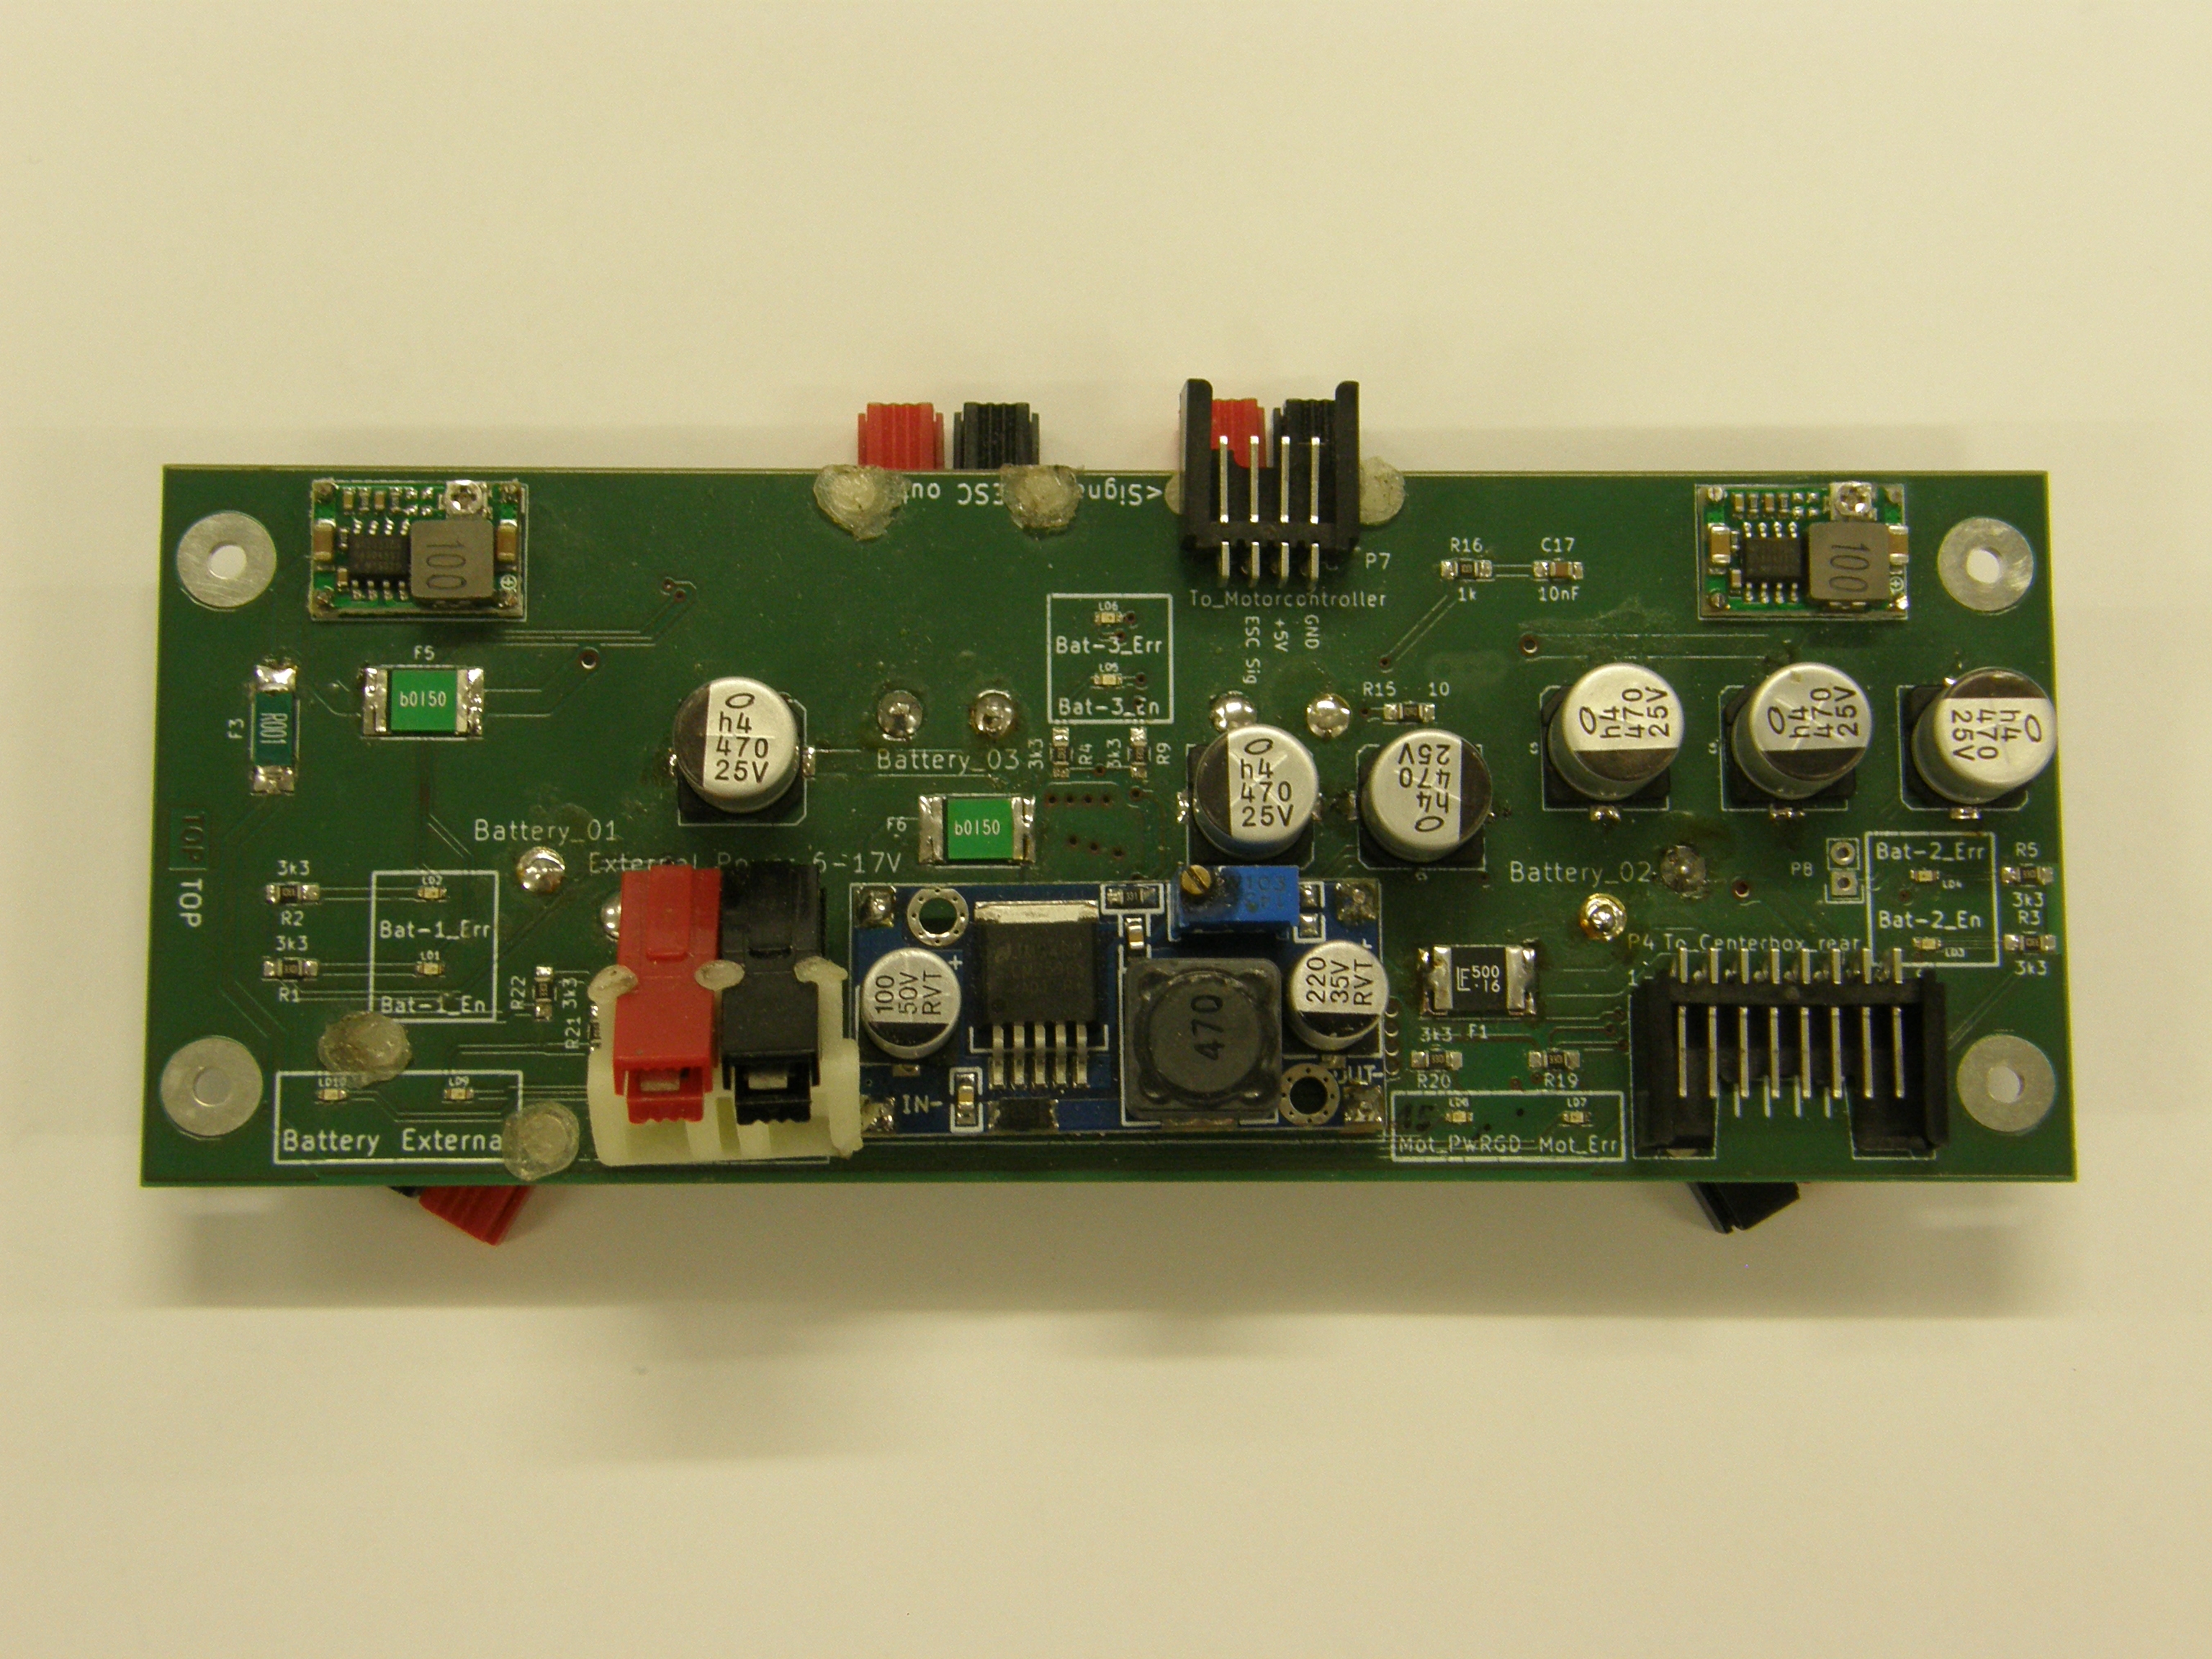
\includegraphics[width=0.9\textwidth]{bilder/Centerbox/Centerbox-Front_Power_AUVSI_2016_Oberseite.jpg} 
\caption{Blick auf die Externen Anschlüsse der AUVSI 2016 Platine} 
\label{fig:Blick auf die Externen Anschlüsse der AUVSI 2016 Platine}
\end{figure}

-->>Schaltplan 2016 


\subsection{Schutz vor Fehlbedienung im Leistungspfad}

Da Fehler abseits von Verbindungsproblemen im Leistungspfad quasi immer zur Beschädigung oder zur Zerstörung des selbigen, mit potentiellem Personenschaden führen, werden für diesen die meisten Sicherheitsmechanismen verwendet.
Hauptsächlich wird das Ideale Dioden System verwendet um einen parallelen Betrieb von Akkus verschiedener Ladungsstände zu ermöglichen.

\subsubsection{Die Ideale Diode}

Die Ideale Diode als Elektronische Schaltung lässt sich in ihrem Schematischen Aufbau mit folgendem Schaltplan darstellen.

\begin{figure}[H]
\centering
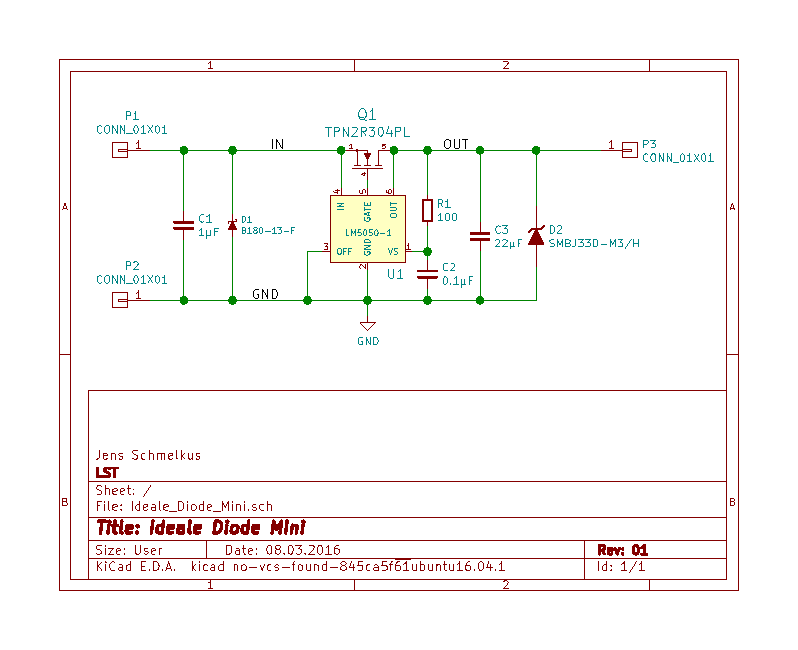
\includegraphics[width=0.9\textwidth]{Schaltplaene/Ideale_Diode_Mini.pdf} 
\caption{Schaltplan der Idealen Diode erster Generation} 
\label{fig:Schaltplan der Idealen Diode erster Generation}
\end{figure}

Grundlegend Besteht der Aufbau aus einem Steuermodul und einem Schalter. Außerdem werden ein und Ausgänge der Aufbaus mit Spannungsdämpfern und Verpolungs- sowie Überspannungsschutz versehen.



\subsubsection{Die Ideale Diode als Modul}

Um eine leichte Integration in möglichst viele Anwendungen zu ermöglichen wurde beim Layout der Platine die kleinstmögliche Abmessung angestrebt. 

\begin{figure}[H]
\centering
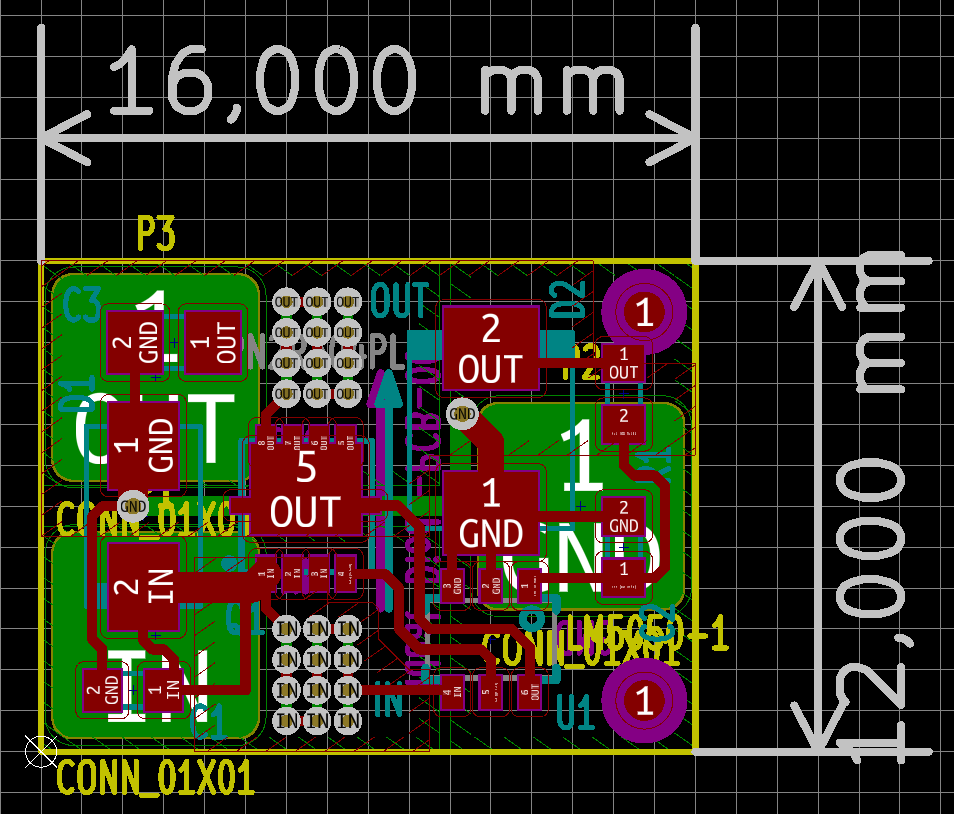
\includegraphics[width=0.9\textwidth]{bilder/Ideale_Diode/Ideale_Diode_Mini_rev01_ver00.png} 
\caption{Layout der Idealen Diode erster Generation} 
\label{fig:Layout der Idealen Diode erster Generation}
\end{figure}

Damit ergab sich in der Montage ein kompaktes Baumaß für die Platine mit all ihren Bauelementen.

\begin{figure}[H]
\centering
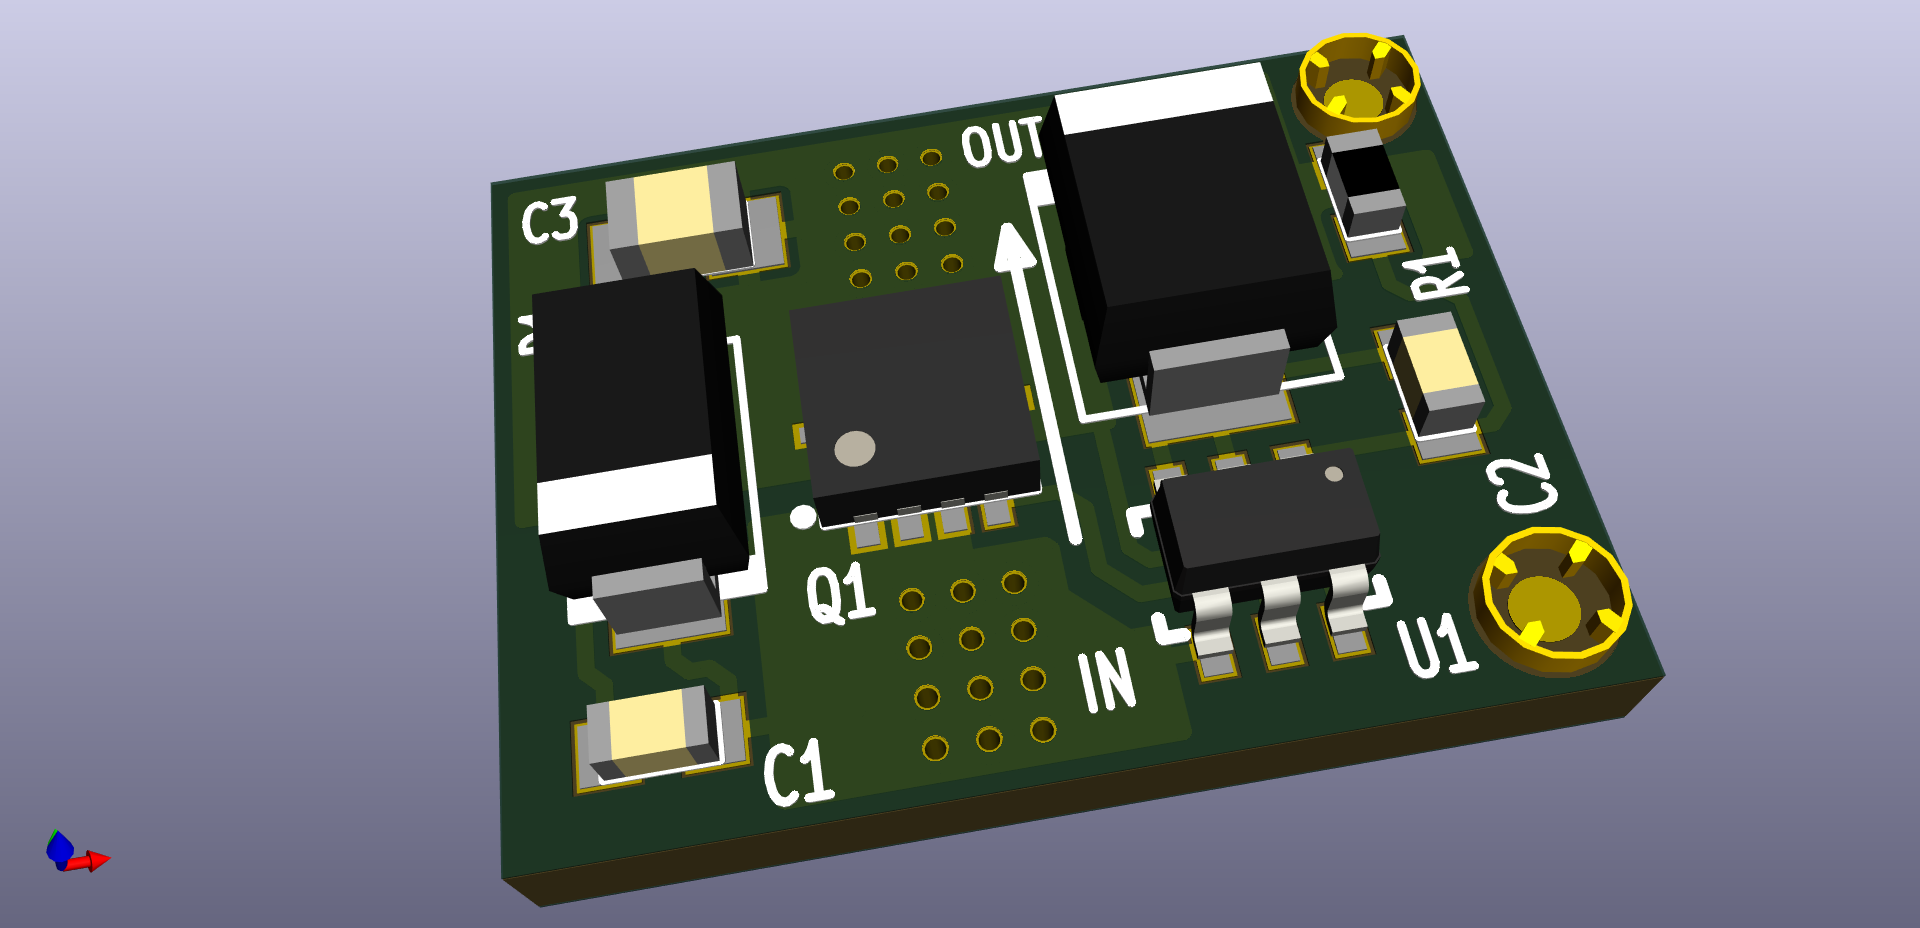
\includegraphics[width=0.9\textwidth]{bilder/Ideale_Diode/Ideale_Diode_Mini_rev01_ver00-3D.png} 
\caption{3D Ansicht der Idealen Diode erster Generation} 
\label{fig:3D Ansicht der Idealen Diode erster Generation}
\end{figure}

\subsubsection{Optimierung der Idealen Diode}

Nach den Messungen zur Verlustleistung an der idealen Diode wurde die Abhängigkeit von Kühlung und Innenwiderstand des Mosfets quantifiziert. 


\begin{figure}[H]
\centering
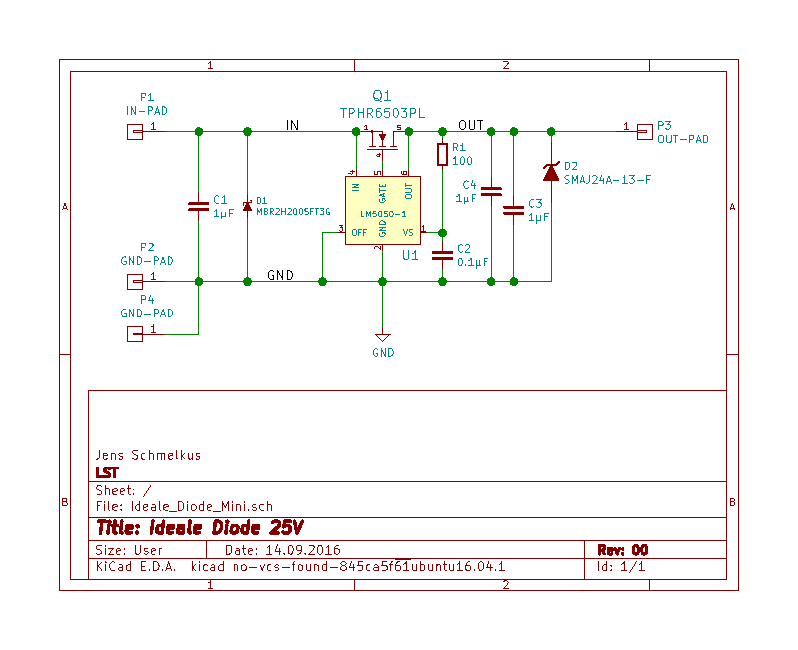
\includegraphics[width=0.9\textwidth]{Schaltplaene/Ideale_Diode_25V_rev00-ver00.pdf} 
\caption{Schaltplan der Idealen Diode zweiter Generation} 
\label{fig:Schaltplan der Idealen Diode zweiter Generation}
\end{figure}


\begin{figure}[H]
\centering
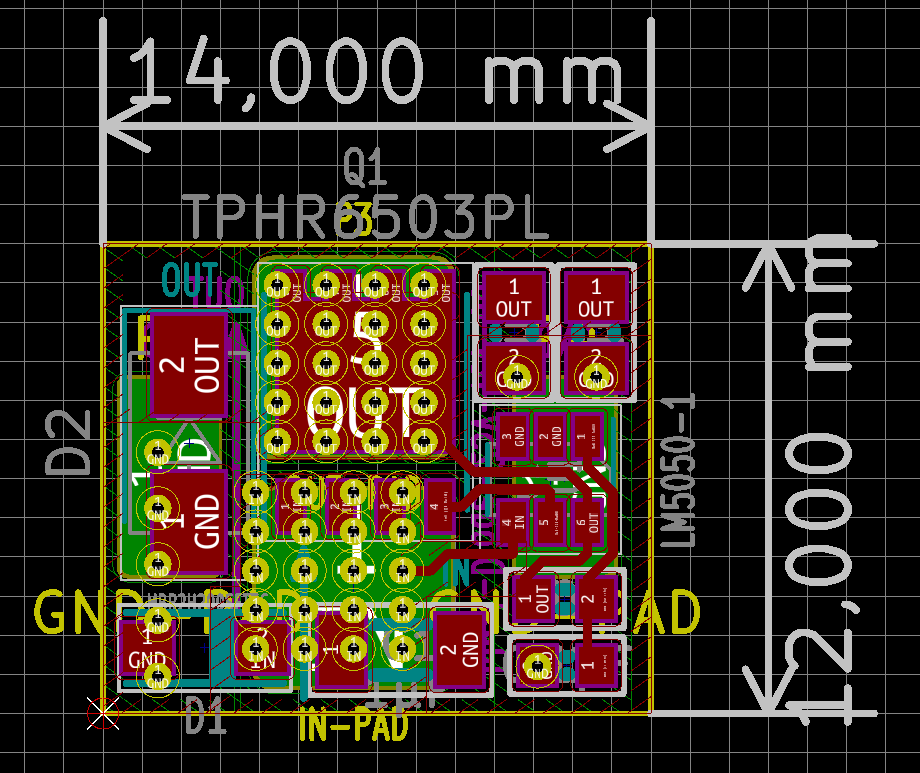
\includegraphics[width=0.9\textwidth]{bilder/Ideale_Diode/Ideale_Diode_25V_rev00_ver00.png} 
\caption{Layout der Idealen Diode zweiter Generation} 
\label{fig:Layout der Idealen Diode zweiter Generation}
\end{figure}



\begin{figure}[H]
\centering
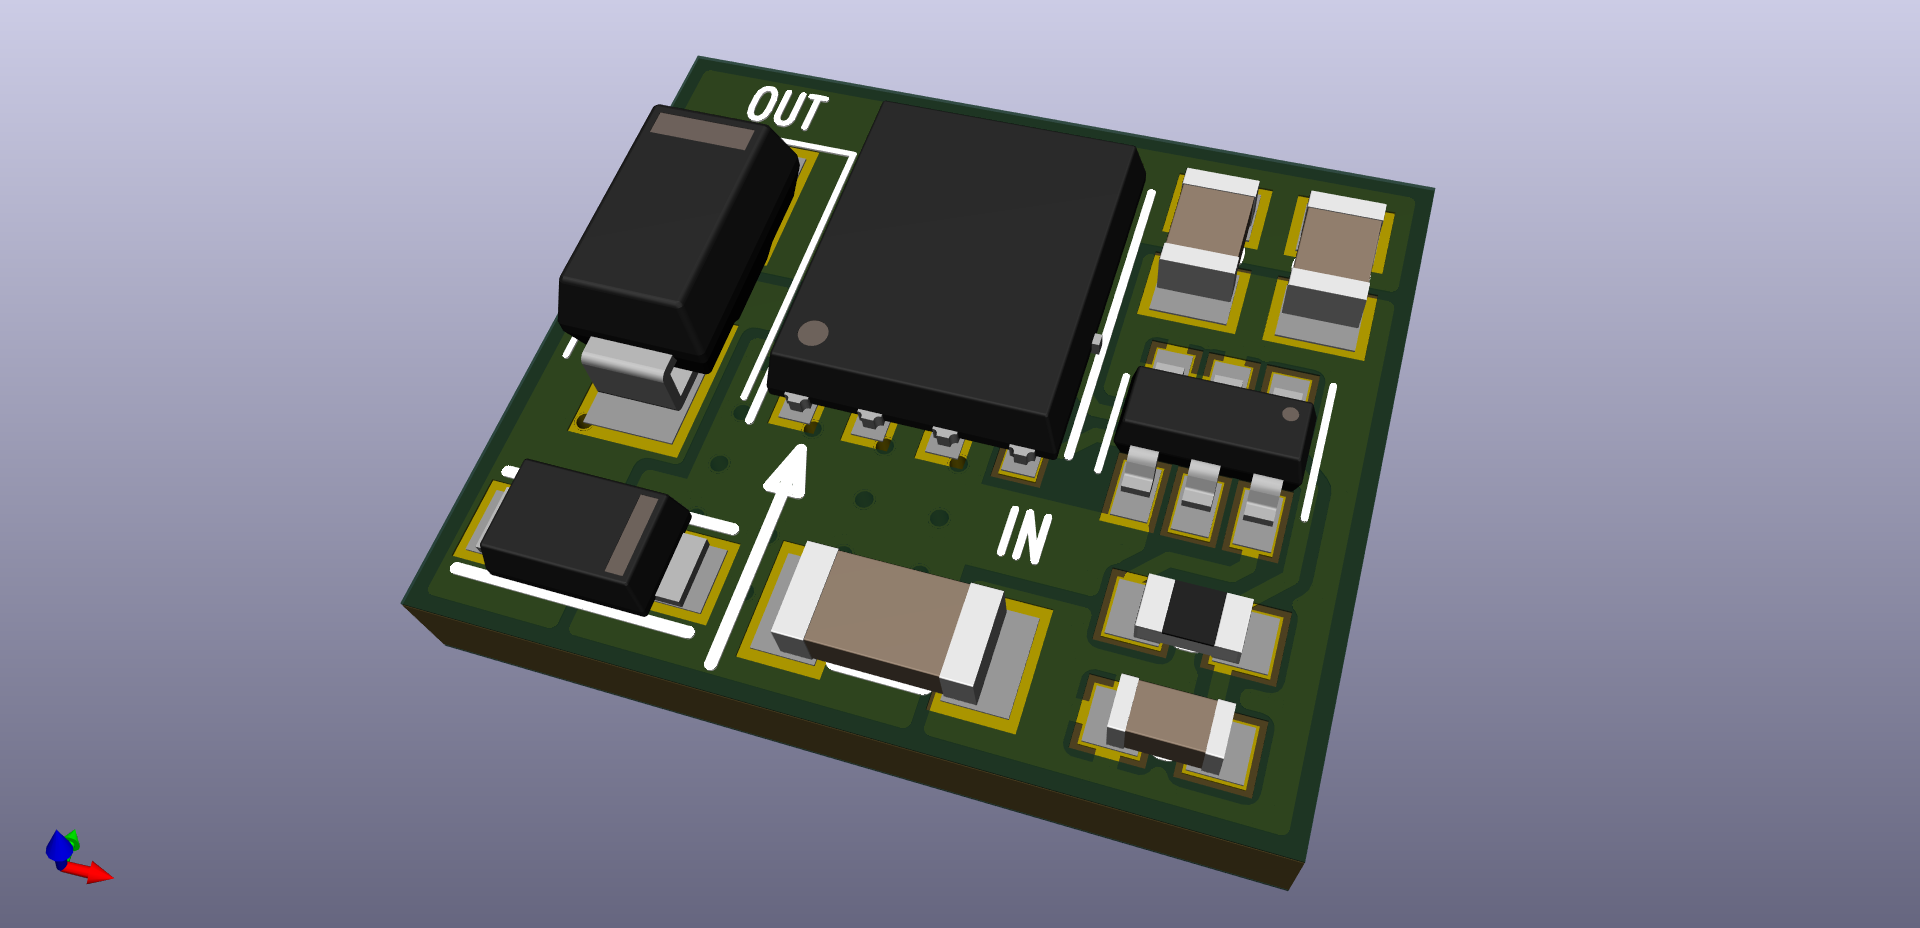
\includegraphics[width=0.9\textwidth]{bilder/Ideale_Diode/Ideale_Diode_25V_rev00_ver00-3D.png} 
\caption{3D Ansicht der Idealen Diode zweiter Generation} 
\label{fig:3D Ansicht der Idealen Diode zweiter Generation}
\end{figure}


\begin{figure}[H]
\centering
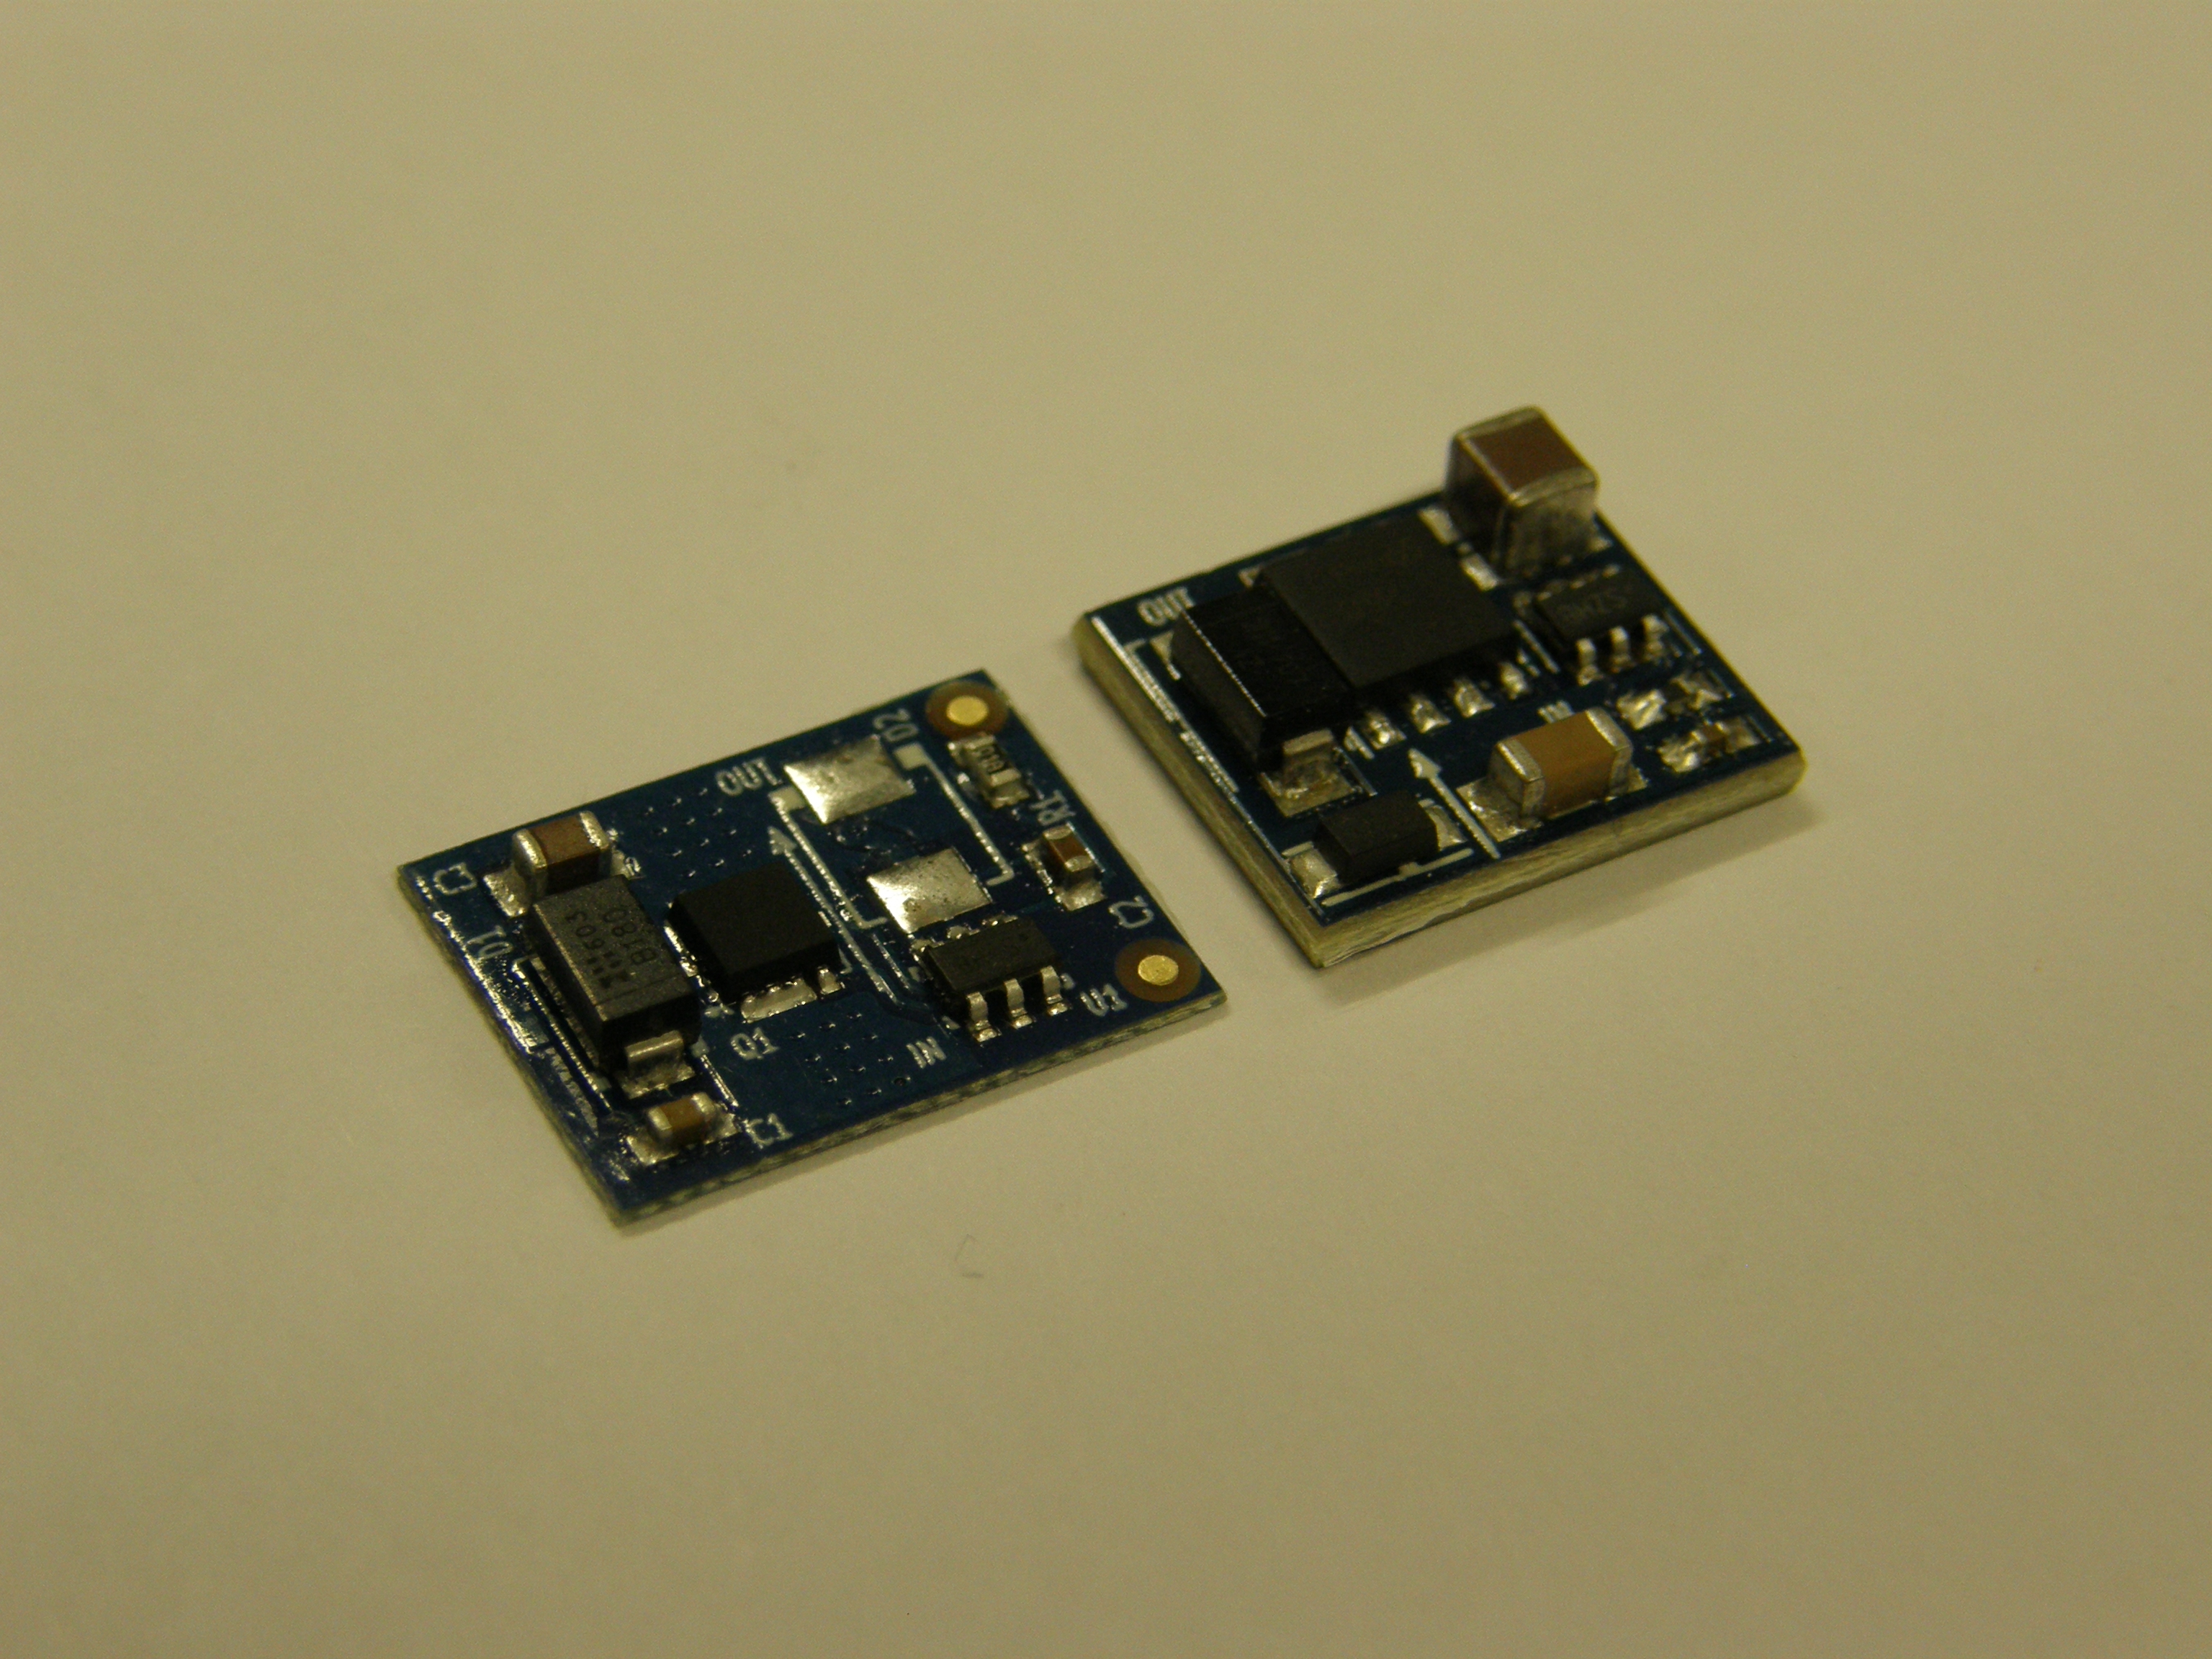
\includegraphics[width=0.9\textwidth]{bilder/Ideale_Diode/Ideale_Dioden_Paar_dreiviertel.jpg} 
\caption{Beide Generationen des Ideale Dioden Moduls nebeneinander} 
\label{fig:Beide Generationen des Ideale Dioden Moduls nebeneinander}
\end{figure}

\section{Integration von Zukaufbaugruppen}


LM2596S  Baugruppe Dc-Dc 
Vin 4 - 35 V 

Vout 1,23 - 30 V einstellbar

3 A  mit Kühlung

meist auf 5V  eingestellt 
Meist 5V Versorgung für Servos

\begin{figure}[H]
\centering
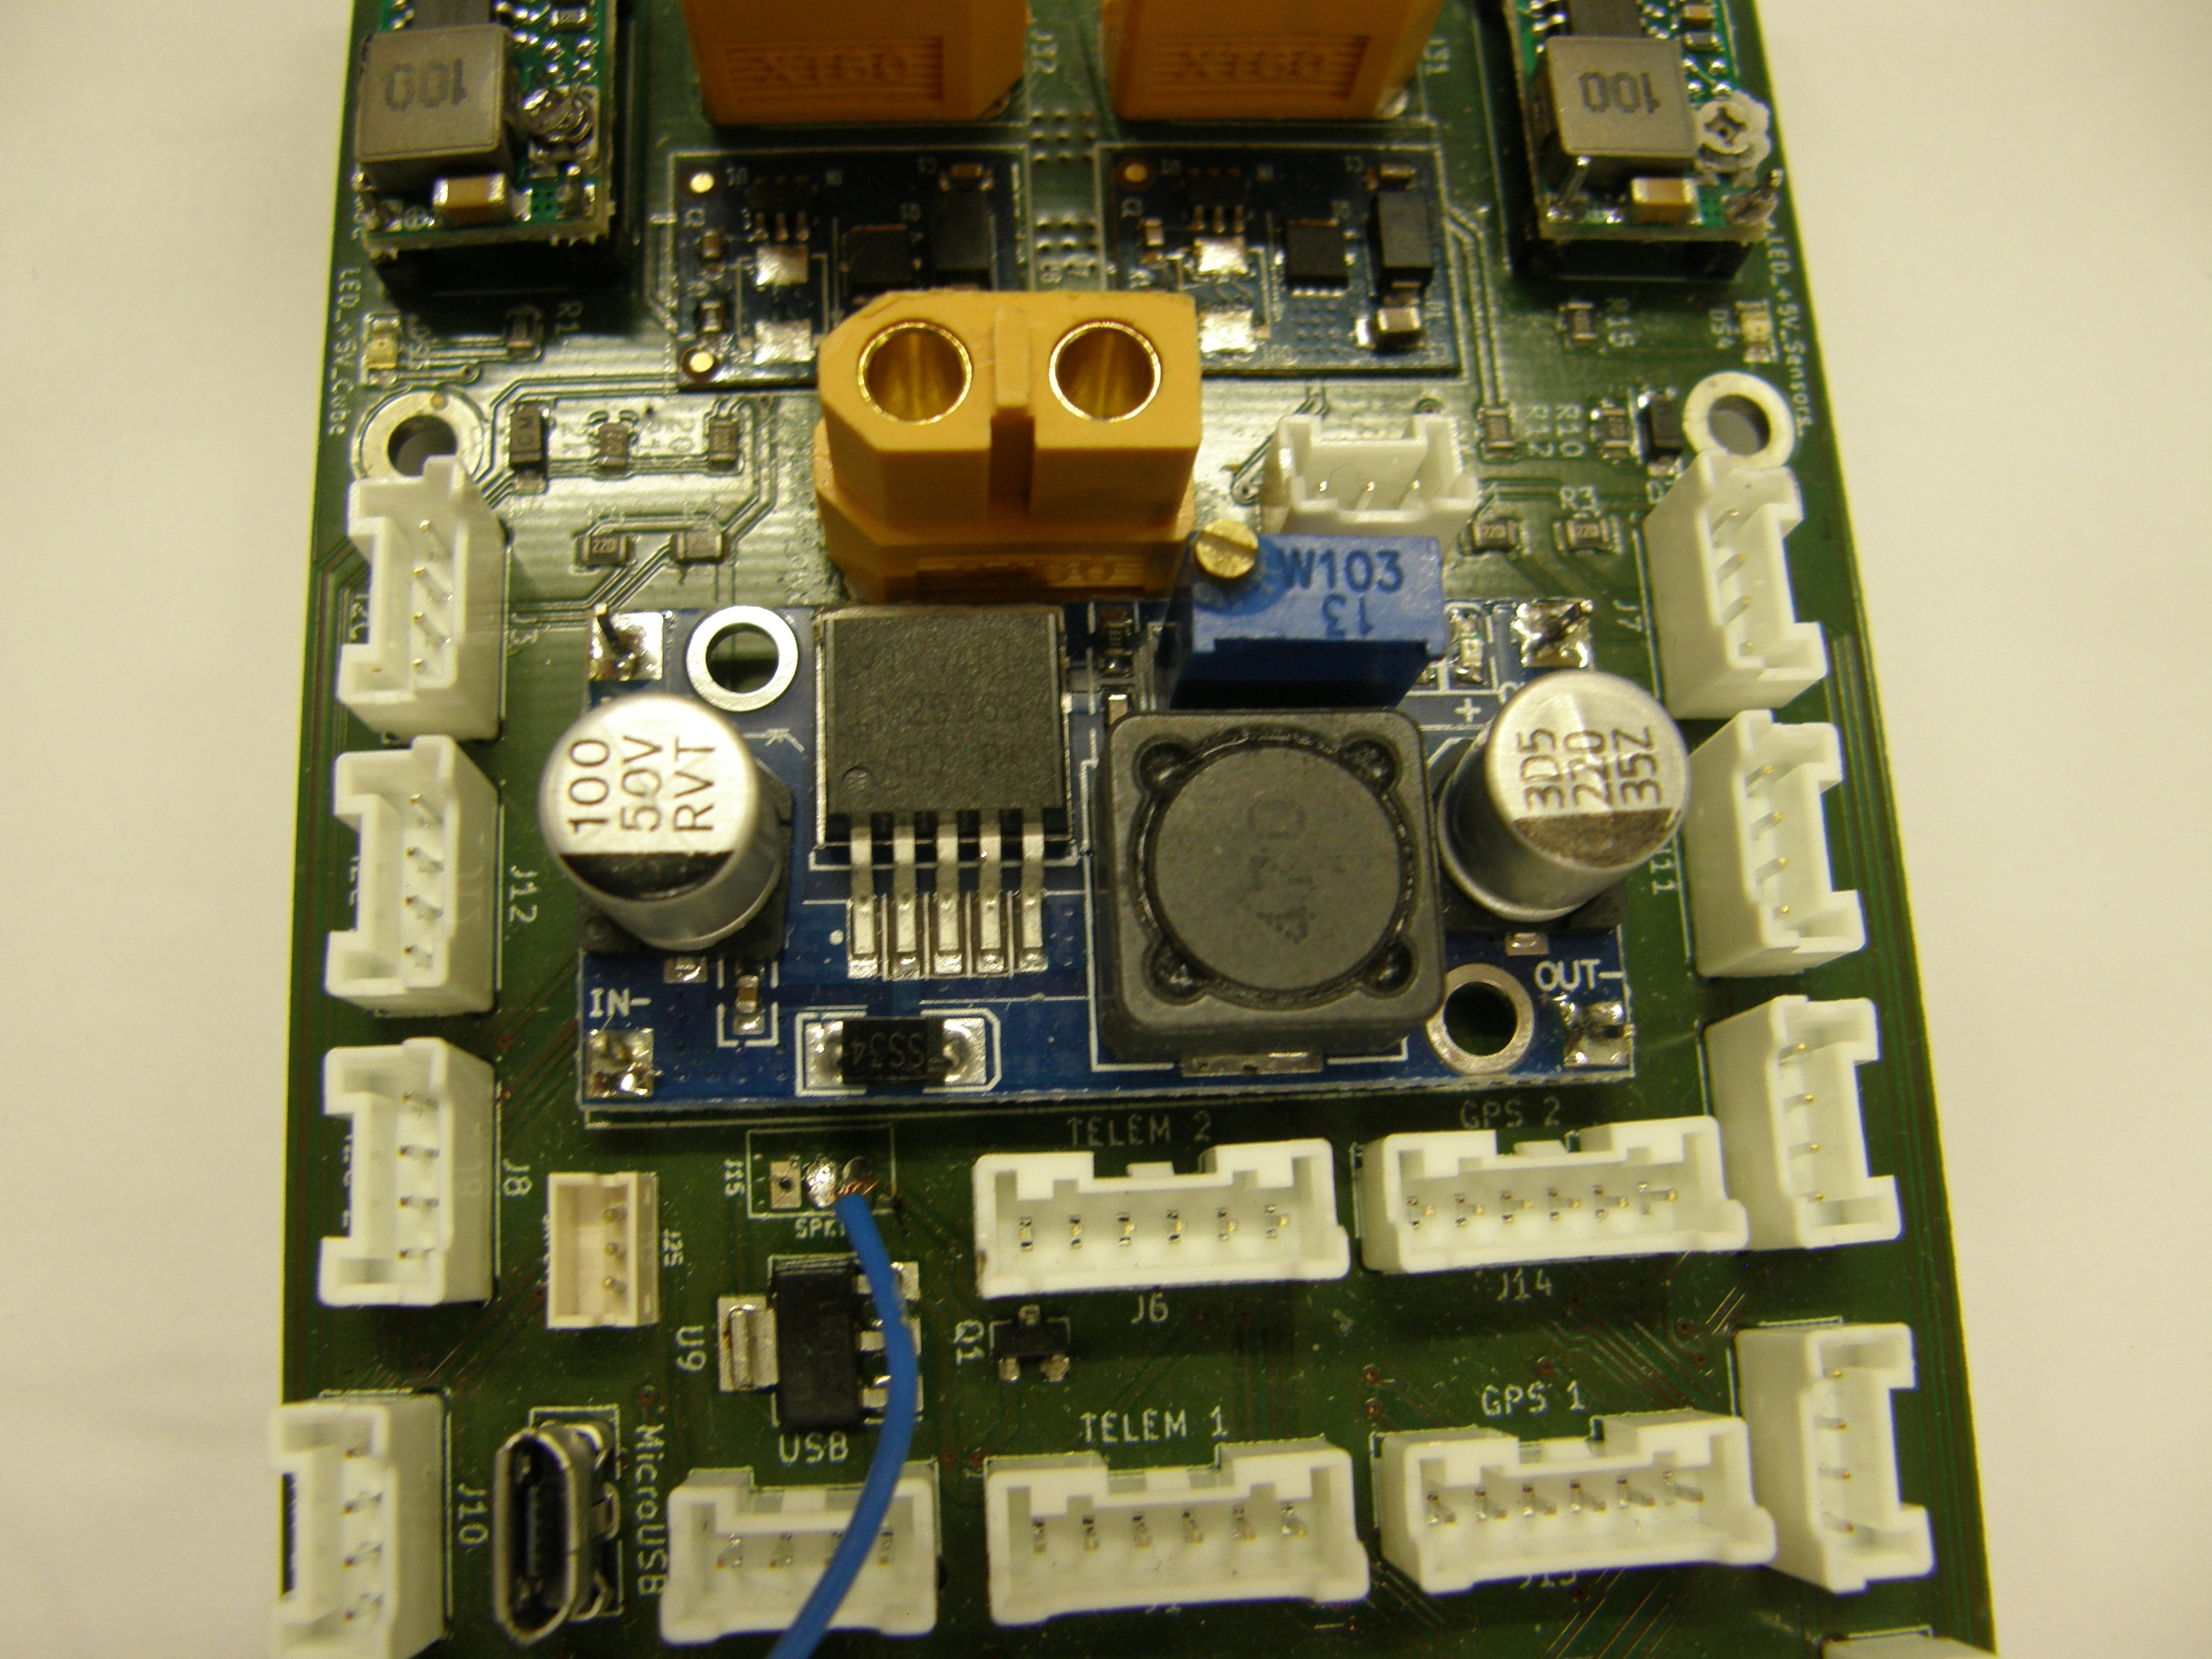
\includegraphics[width=0.9\textwidth]{bilder/Zukaufbauteile/Baugruppen_Dc-Dc_LM2596S.jpg} 
\caption{Zugekauftes Dc-Dc Wandler PCB mit LM2596} 
\label{fig:Zugekauftes Dc-Dc Wandler PCB mit LM2596}
\end{figure}


DSN Mini 360  Baugruppe Dc-Dc

Vin 4,75 - 23 V

Vout 1,0 - 17 V einstellbar

Iout dauer  ~ 1,5 A

Meist 5 V versorgung für Pixhawk und Lidar

\begin{figure}[H]
\centering
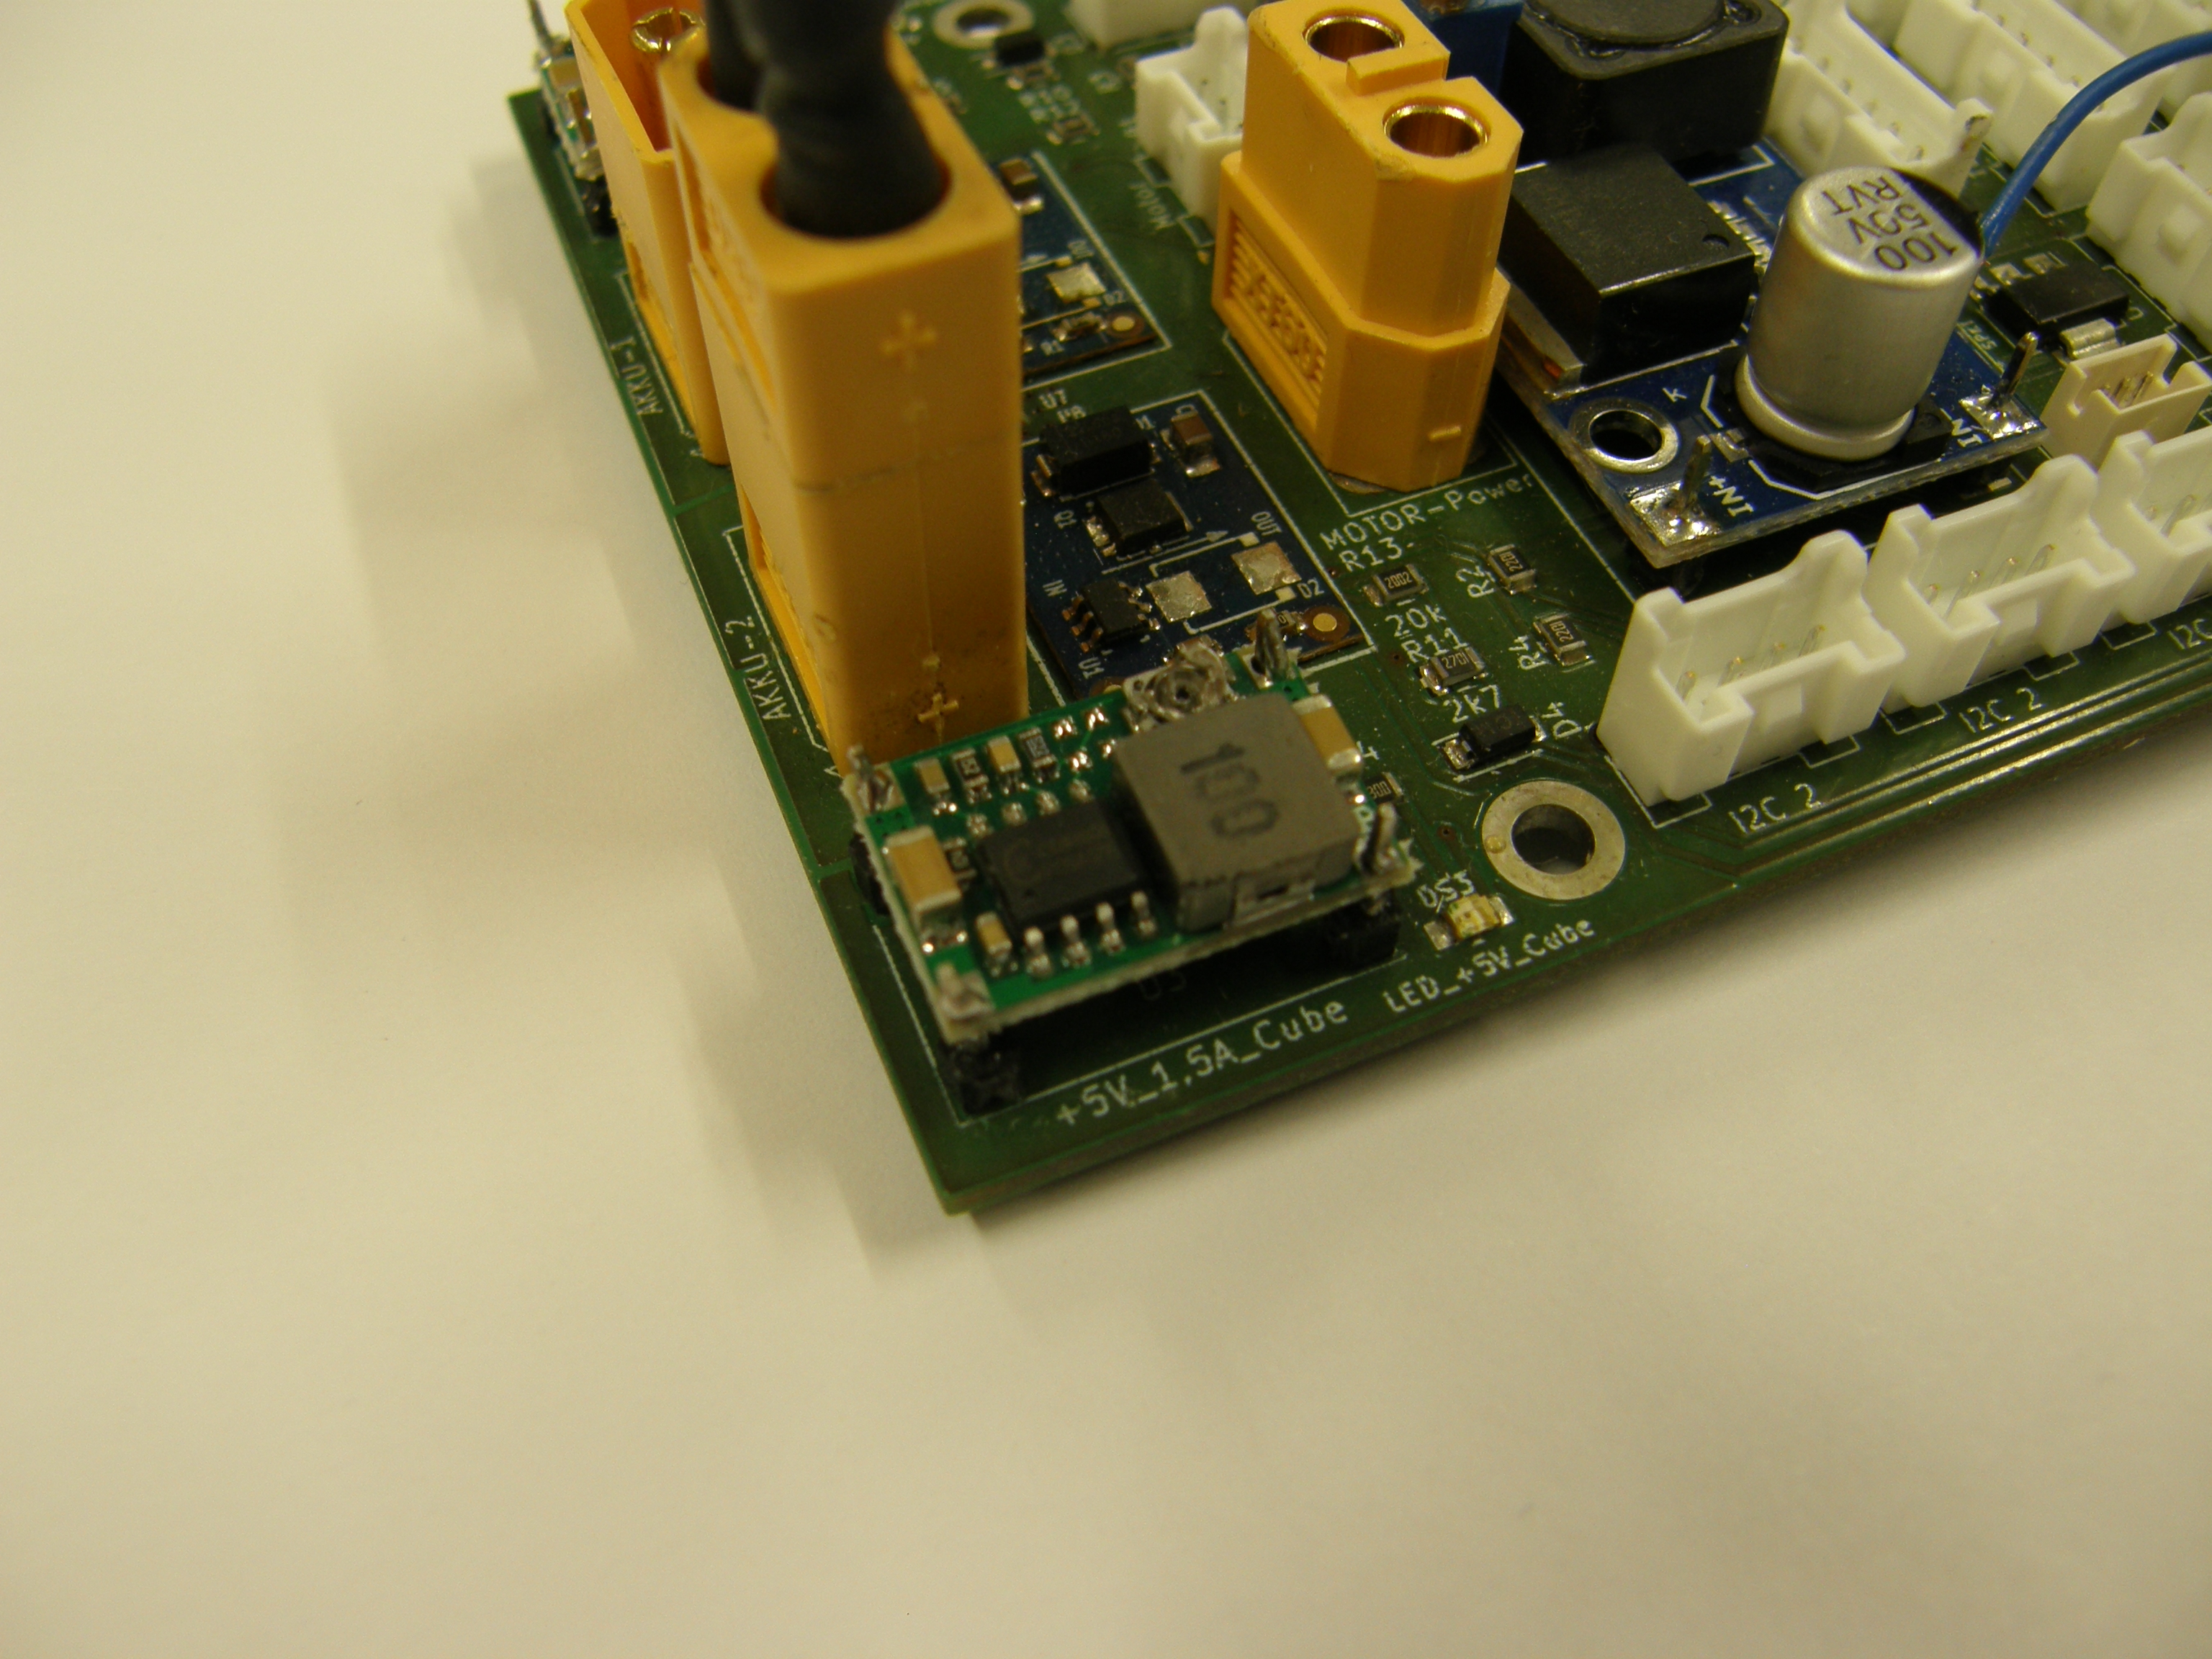
\includegraphics[width=0.9\textwidth]{bilder/Zukaufbauteile/Baugruppen_Dc-Dc_Mini-360.jpg} 
\caption{Zugekauftes Dc-Dc Wandler PCB Mini-360} 
\label{fig:Zugekauftes Dc-Dc Wandler PCB Mini-360}
\end{figure}

\section{Mechanische Integration im Flugsystem}

\begin{figure}[H]
\centering
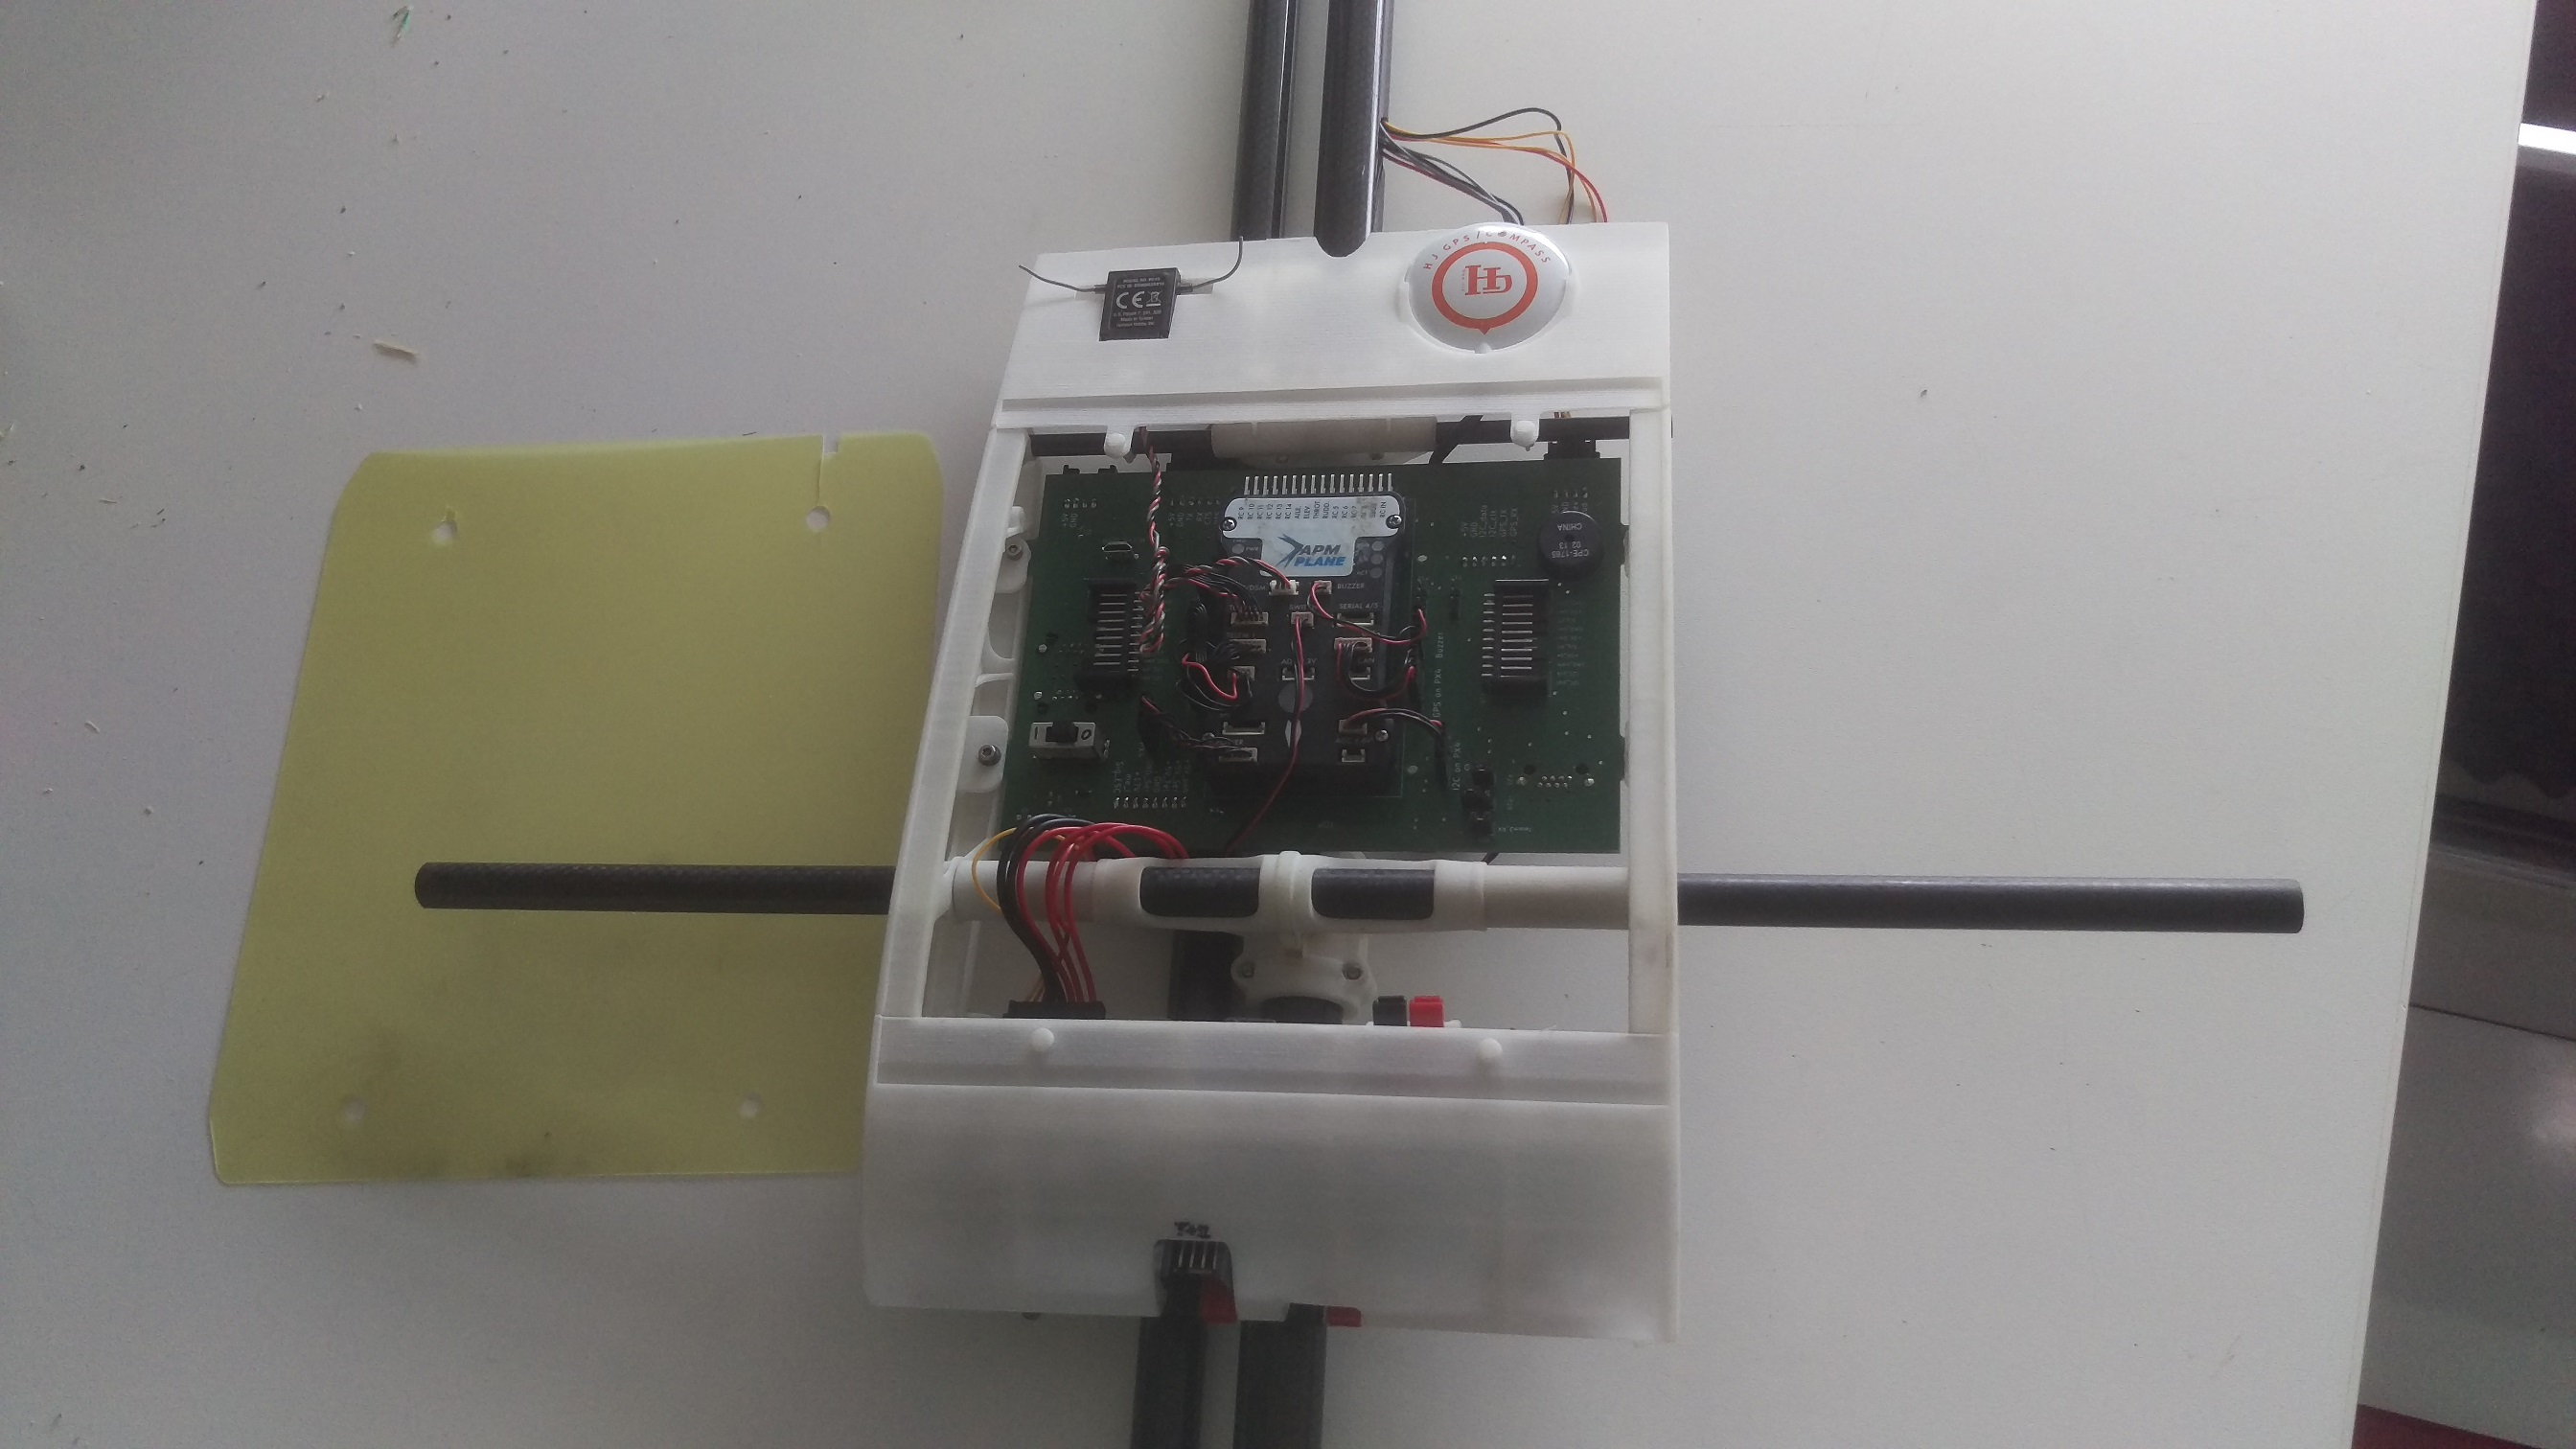
\includegraphics[width=0.9\textwidth]{bilder/Fotos/AUVSI_2016_Centerbox_Detail.jpg} 
\caption{In der WingCenterBox eingebaute Autopilotenplatine} 
\label{fig:In der WingCenterBox eingebaute Autopilotenplatine}
\end{figure}

\cleardoublepage

%\chapter{Fortschreitende Platinenentwicklung}\label{cha:Platinenentwicklung}

\section{Leistungsplatine}

\subsection{Schaltplan}

\subsection{Platinenlayout}

\section{Autopilotenplatine}

\subsection{Schaltplan}

\subsection{Platinenlayout}

\section{Platinenzusammenbau}

\cleardoublepage

\chapter{Erprobung im Labor}\label{cha:Erprobung im Labor}

Nach den anfänglichen Erfahrungen mit Ausfällen von Elektronik und Mechanik bei den ersten Generationen des Flugzeugs, werden alle Komponenten vor dem Einbau einzeln und nach der Montage als System im Labor getestet.
So können der Schadensumfang im Fehlerfall minimiert werden und die Emulation einzelner Betriebsszenarien ermöglicht eine einfache Eingrenzung möglicher Fehlerquellen.
In der Regel werden Szenarien wie die Maximalleistungsaufnahme beim Start und beim  Steigflug sowie das Langzeitverhalten im Reiseflugzustand nachgestellt. Dabei werden relevante Parameter wie Temperatur der Bauteile gemessen und mit den Erwartungen verglichen.

\section{Einzeltests von Baugruppen}

Vor dem Einbau in das Gesamtsystem werden sowohl die einzelnen Platinen als auch ihre Modul Platinen einzeln Ddrchgetestet.
Dazu wird für die Leistungssysteme ein Labornetzteil als Quelle verwendet welches 0 - 45 V und 0 - 50 A zur Verfügung stellen kann.
Der theoretische Nutzbereich des 4-zelligen Akkusystems von 4,20 V bis 3,00 V je Zelle \footnote{\cite[Seite~1.12f.]{Reddy2010}} stellt einen Operationsbreich von 16,8 V bis 12,0 V bereit. Deshalb wird für die meisten Tests eine mittlere Spannung von 14,5 V gewählt. Der Strom wird auf etwa 30 A begrenzt um mögliche Fehlerfolgen zu begrenzen.
Die als kritisch eingestuften Bauteile werden mit Thermoelementen vom Typ K beklebt. Außerdem wird eine FLIR Thermokamera mit einer Auflösung von 320x240 Pixel fest aufgestellt, um die globale Themperaturverteilung auf dem PCB zu beobachten.
Da die absolute Genauigkeit der Temperaturwerte der Wärmebildaufnahmen aufgrund des ungekühlten CCD zumeist nicht korrekt sind, werden diese mit Hilfe der genauen Werte der K Elemente skaliert.
Die Temperatur ist in unserem Leistungsbereich die primäre Schadensursache. 
Um eine vergleichbare Kühlungssituation aller getesteten Bauteile zu realisieren, werden diese in der Ebene in ruhiger Luft vermessen und auf Referenz-Grundplatinen montiert.
Dies ermöglicht eine konservative Einordnung des Betriebspunktes, da im Flugbetrieb alle Elektronikkomponenten vom Fahrtwind überspült werden und damit von einer verbesserten Kühlung auzugehen ist.

\subsection{Ideale Diode}

Die Messungen an dem Aufbau des Moduls der Idealen Diode beschränken sich auf das Verhalten als Leistungsbauteil. 
In Anlehnung an die Referenz-Testaufbauten welche von Texas Instruments, Vishay Semiconductors und Toshiba Power Electronics für einzelne Mosfets in den zugehörigen Datenblättern verwendet werden, ist auch die Adapterplatine für alle Idealen Dioden gestaltet.
Die Platine misst 1x1 Zoll mit 35 um Kupferstärke und regulärem Lötstopplack. Die Ein- und Ausgänge sind über Powerpol 55A Steckverbinder realisiert. SMD montierte Ösen ermöglichen den Abgriff der Differenzspannung über das gesamte Ideale Dioden Modul. In Einzelfällen wird zum Vergleich der Spannungsabfall über den reinen Mosfet manuell zum Vergleich gemessen.

Die vergleichende Messung der beiden Generationen und verschiedener Mosfet-Bestückungen zeigt die unterschiedlichen equivalenten Widerstände über den durchgeleiteten Strom.
Dieser Strom ist unmittelbar nach den Ohmschen Gesetzen für die örtliche Verlustleistung und damit für die Erwärmung der Baugruppe verantwortlich.


\begin{comment}


\begin{figure}[H]
\begin{tikzpicture}
 \begin{axis}[
 	ymin=0,
    xmin=0,
 	width=\textwidth,height=0.5\textheight,
  	%title=Einfahrzyklus Wegprofil,
    xlabel={Testsrom [A]},
    ylabel={R-res [mOhm]},
    grid=major,
    legend entries={Ideale Diode Mini,Ideale Diode Mini mod.,},
    enlarge x limits=0.01,
]
 	\addplot+[mark=*] table[x=Teststrom1, y=Ideale_Diode_Mini1]  {graphen/Testdaten_Ideale_Dioden-Vergleich.txt};
 	%\addplot+[mark=x] table[x=Teststrom2, y=Ideale_Diode_Mini2]  {graphen/Testdaten_Ideale_Dioden-Vergleich.txt};

 \end{axis}
\end{tikzpicture}
\caption{Einfahrzyklus Wegprofil (für jeden Zyklus ist ein Hub dargestellt)}
\label{Einfahrzyklus_Wegprofil}
\end{figure}


\end{comment}



\begin{figure}[H]
\centering
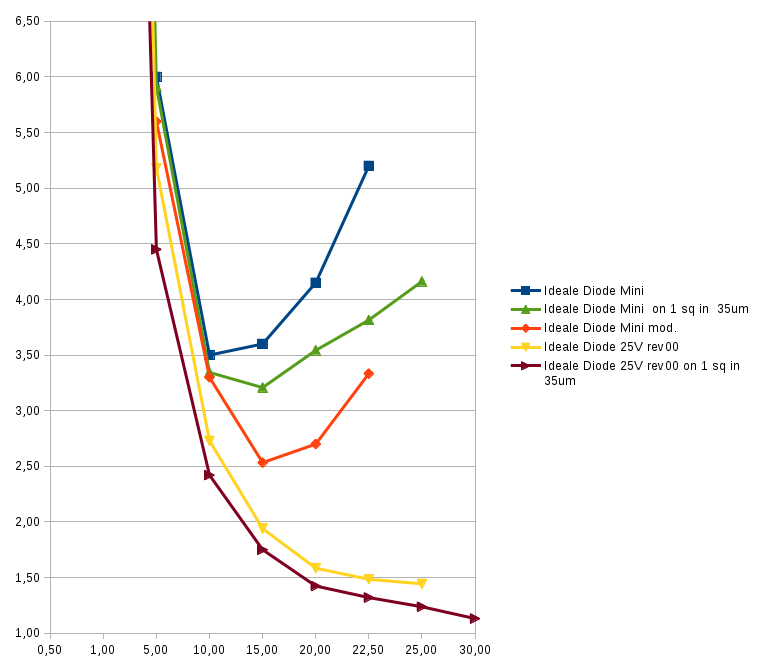
\includegraphics[width=0.9\textwidth]{graphen/Wiederstand-Strom-Ideale_Diode_ver00} 
\caption{Widerstandsverlauf} 
\label{fig:Widerstandsverlauf}
\end{figure}


Wie aus der Grafik \ref{fig:Widerstandsverlauf} ersichtlich wird, ist der Mosfet, wie erwartet, als zentrales Schaltelement für quasi den gesamten Widerstand verantwortlich.
Eine Modifikation der ersten Diodengeneration mit dem Austausch des Mosfet TPN2R304PL mit einem Nennwiderstand von 1,8\,$m\Omega$ \cite{TPN2R304PL} durch den Mosfet FDMC012N03 mit einem Nennwiderstand von 1,36\,m$\Omega$ \cite{FDMC012N03} reduziert den equivalenten Widerstand bei einem üblichen Akkustrom von 10 A im Dauerbetrieb von 3,5\,$m\Omega$  auf 3,2\,$m\Omega$.
Demgegenüber stellt die zweite Generation eine deutliche Widerstandsersparnis dar.
Erreicht wird diese durch ihre optimierte Wärmeableitung mit Neuanordnung der Bauteile und Verkleinerung des PCB sowie der nochmals veränderten Wahl des Mosfets auf TPHR6503PL.

Der höchste Dauerstrom liegt bei der unmodifizierten Generation 1 bei 20\,A und bei der Generation 2 bei 30\,A. 
Generell wird der höchste Dauerstrom über die Baugruppe durch einen kleinstmöglichen Innenwiderstand des verwendeten Mosfets und die Kupferfläche begrenzt, auf welcher das Modul montiert is,t um Wärme abstrahlen zu können. Das Modul PCB selbst hat aufgrund seiner geringen Größe eine vernachlässigbar kleine Kühlleistung.

Das Bild \ref{fig:Beide Generationen des Ideale Dioden Moduls nebeneinander} zeigt zum Vergleich auch das Modul ohne Adapterplatine.

\subsection{5 Volt Servoversorgung}

Um die Eignung der zugekauften 5 V Spannungswandler zu evaluieren, wurde exemplarisch ein Wandler mit einem Servo impulsmäßig belastet.
Dabei wurde das Dc-Dc Modul mit 14,5 V versorgt und an den auf 5,0 V eingestellten Ausgang ein Servo angeschlossen. Der Servo wurde von einem Servo Testgerät mit Steuersignalen versorgt, welche ihn im Wechsel zu den jeweiligen Extrempositionen seines Verfahrbereichs dirigieren. 
An den 5,0 V Ausgang des Wandlers und das in den Servo laufende PWM Signal wurde ein  Digitaloszilloskop angeschlossen. Damit  wurde der Einbruch der 5 V Spannung, unter der impulsartigen Strombelastung, des im Umkehrpunkt beschleunigenden Servos beobachtet.
Damit sollte beurteilt werden, ob der durch die Regelgeschwindigkeit und die begrenzte Ausgangskapazität des Wandlers unvermeidbare kurzzeitige Einbruch im Millisekundenbereich in der Spannungsversorgung der Servos kritische Zustände verursacht.
Es könnte beispielsweise ein zeitgleiches Ausschlagen mehrerer Servomotoren dazu führen. dass die Spannung so weit absinkt, dass keiner der Motoren noch funktionsfähig ist, beziehungsweise die Verfahrgeschwindigkeit deutlich absinkt.

Die Messung ergab einen kumulierten Einbruch der Spannung  unter ca. 0,5 V. 
Damit kann das Verhalten in allen erwarteten Flugsituationen als unkritisch bewertet werden. Gegebenenfalls wird hier in Zukunft zur weiteren Absicherung des Verhaltens noch eine Stützung mit Elektrolythkondensatoren umgesetzt. 

\section{Evaluierung der Signalpfade}

Es sollten Fehler im Schaltplan und im Routing der Platine ausgeschlossen werden. Dafür erfolgte ein Test der korrekten Signalführung ohne Einsatz der Sensoren und der Pixhawk Autopiloten Hardware. Dazu wurden an die Aus- und Eingänge des Pixhawk und der Sensoren ein 1 khz 50 Prozent PWM Signal angelegt, um mit dem Oszilloskop die jeweils vorgesehene Gegenstelle zu überprüfen.

Dabei konnten auf der Autopiloten-Platine keine Fehler festgestellt werden.
Auch die Inbetriebnahme der Sensoren und des Autopiloten verlief Hardwareseitig problemlos.

\section{Überprüfung der Logikfunktionen der Leistungsplatine}

Um eine einwandfreie Funktion und damit den sicheren Betrieb der Leistungsplatine sicherzustellen wurden deren Schutz und Regelfunktionen einzeln getestet.
Es wurden zunächst von einem Paket, aufsteigend, alle Permutationen an Spannungsquellen an die drei vorgesehenen Anschlüsse gekoppelt und die korrekte Führung der Energie überprüft.
Es wurde die vorgesehene Statusindikation durch Leuchtdioden verschiedener Farben dokumentiert.
Die reguläre Führung der Quellen, Blockierung der Flugakkus im Bodenbetrieb und die Anzeige der Energiepfade funktionierte korrekt.

\section{Testlauf der Leistungsplatine}

Anschließend wurde die Platine in den Eingangs beschriebenen Flugmodi im Dauerlauf getestet.
Bei den Tests im Startleistungsbereich stieg der Strom dabei auf einen Wert an, der dazu führte, dass der Sicherungsschalter in Richtung Motorversorgung abschaltete.
Dies führte zu einer Oszillation des zugehörigen Mosfets zwischen Sperr- und Leitzustand. Der in diesem Übergangsbereich hohe Innenwiderstand und der damit verbundene hohe Leistungsabfall am Mosfet führte bereits nach kurzer Zeit zur dessen Zerstörung durch Überhitzung.
Alle weiteren Versuche, dieses Verhalten durch Dämpfung der Abschaltzeitschwelle oder Verbesserung der Kühlung zu vermeiden, blieben erfolglos. Deshalb wurden aufgrund der geringen verbleibenden Zeit bis zum Wettbewerb diese Schaltung ersatzlos entfernt und mit einer entsprechenden Drahtbrücke überbrückt.

\cleardoublepage

\chapter{Einsatz in der Flugerprobung}\label{cha:Einsatz in der Flugerprobung}

\section{Auftretende Fehler}

\subsection{Überstrom im Motortestlauf}

\subsection{Überspannung der 5 Volt Schiene}

\section{Anpassung des Elektronikonzepts}

\section{Anpassung der Bedienvorgaben}

\section{Fazit der Flugerprobung}

\cleardoublepage

%\chapter{(optional) Einsatz auf dem Wettbewerb}\label{cha:Einsatz auf dem Wettbewerb}

\section{Präsentation und Vergleich mit den Wettbewerbern}

\section{Ergebnis der Flugaufgabe}

\section{Wettbewerbserfolg}



\cleardoublepage

\chapter{(optional-kurz) Weiterentwicklung}\label{cha:Weiterentwicklung}

\section{Erfahrungen aus dem Feldeinsatz}

\section{Anpassung der Anforderungen an die Elektronik}

\section{Detailverbesserungen an den Komponenten}

\section{Technischer Ausblick}

\cleardoublepage

\chapter{Fazit und Ausblick}\label{cha:Fazit und Ausblick}

In den letzten Jahren hat sich die Elektronik des Automatischen Flugsystems des Labor für Systemtechnik sich seinen vielfältigen Aufgaben Angepasst.
Dabei hat sich sowohl die Augabenformulierung und das Konzept von ersten Versuchen nahe einem klassischen Modellflugzeug zu einem vollständigen System mit  Platinenaufbau und zahlreichen Unteraufgaben gewnadelt. Es ist ein vielfältiges Repatoire an erprobten und gereiften Elektronikbaugruppen entstanden welche sich in stetiger optimierung befinden. Damit ist sowohl eine schnelle Anpassung der Gesamten Elektronik an neue Aufgaben und Dimensionierungen möglich.
Damit hat die Elektronik die vorausgegangene Entwicklung der Mechanischen Aufbaus nachvollzogen welche auch eine gezielte Verbesserung einzelner Funktionen bei begrenztem Arbeitsaufwand ermöglicht.
Ebenfalls ist mit dem gewachsenen Erfahrungen mit dem Einsatz des Flugsystems im Zusammenspiel mit den Elektronischen Schutzmaßnahmen ein hohes Sicherheitsniveau für Bedienmannschaft und Flugzeug gewährleistet. Dies hat sich besonders im oft hektischen Wettbewerbseinsatz als wertvoll erwiesen.

Wie das Kapitel der weiteren Entwicklungen bereits aufzeigt entstehen auch abseits der eigentlichen Schaltungsentwicklung neue Ansätze und Aspekte um Handhabung und Leistungsfähigkeit des Gesamtsystems zu steigern.

Somit wird das Elektronische Gesamtsystems des Automatischen Flugsystems des Labor für Systemtechnik auch in den kommenden Jahren kokurrenzfähig auf dem AUVSI Wettberwerb antreten können, als sich auch kurzfristig in Forschungseinsätzen bewähren.




\cleardoublepage

% Setze Numerierung wieder auf römisch zurück und setzte von oben fort
% Wert ist demnach der von 'roemisch'
\newpage
%\pagenumbering{Roman}
%\setcounter{page}{\value{roemisch}}


\printbibheading[title=Quellenverzeichnis]
\printbibliography[heading=none]
%\printbibliography[keyword=Literatur, heading=subbibliography, title={Literaturverzeichnis}]
%\printbibliography[keyword=Quelle, heading=subbibliography, title={Quellenverzeichnis}]

%
% Abbildungsverzeichnis
%
\listoffigures

%
% Tabellenverzeichnis
%
\listoftables

\cleardoublepage


%\begin{comment}
% Appendix, falls vorhanden
\appendix
%% Anhänge, beliebig, kein Zwang
\chapter{Anhang}

% \colorbox{orange}{Datenblätter, Listen, Bedienungsanleitungen, Controller, im Text vorne drauf hinweisen, gleiche Messungen in den Anhang, Ergebnisse vorne}




%\clearpage

\section{Beurteilung von Lastenhandhabungen anhand von Leitmerkmalen}\label{cha_Anhang_5}

\clearpage

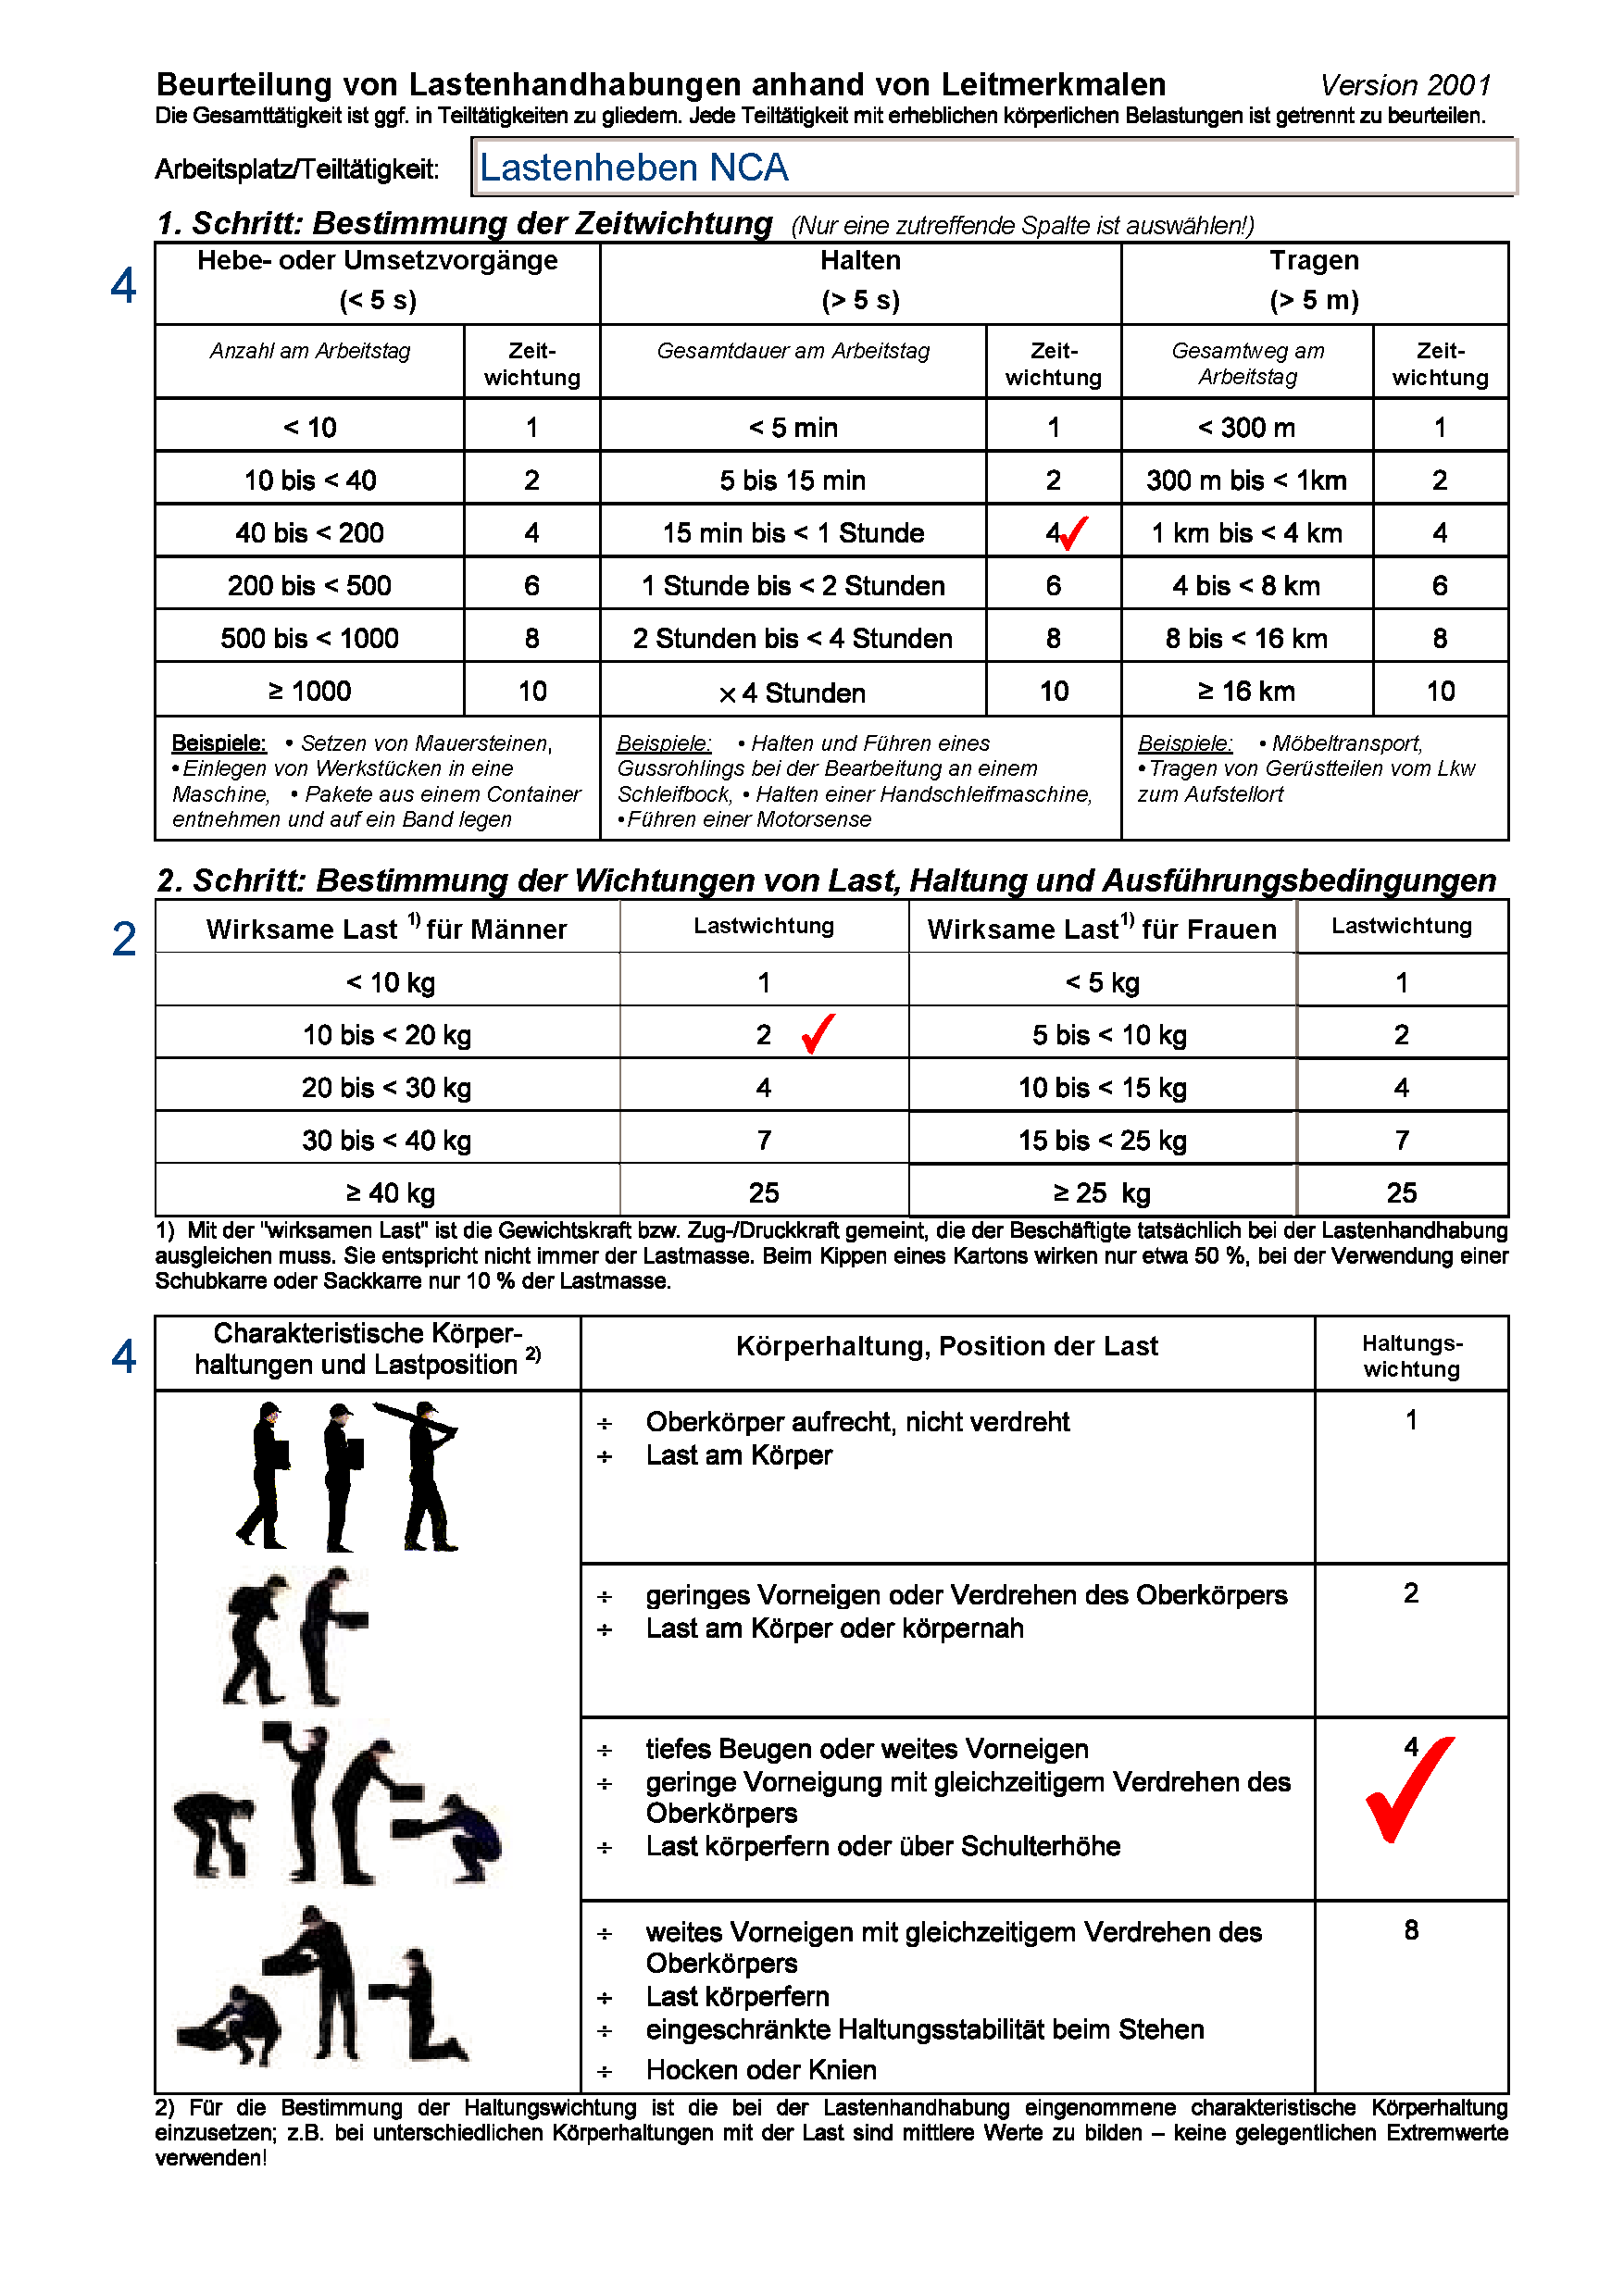
\includegraphics[page=1,width=\textwidth]{anhang/LMM-Heben-Halten-Tragen.pdf}

\clearpage

\includegraphics[page=2,width=\textwidth]{anhang/LMM-Heben-Halten-Tragen.pdf}


\section{Überblick über NC-Aggregate}\label{cha_Anhang_4}



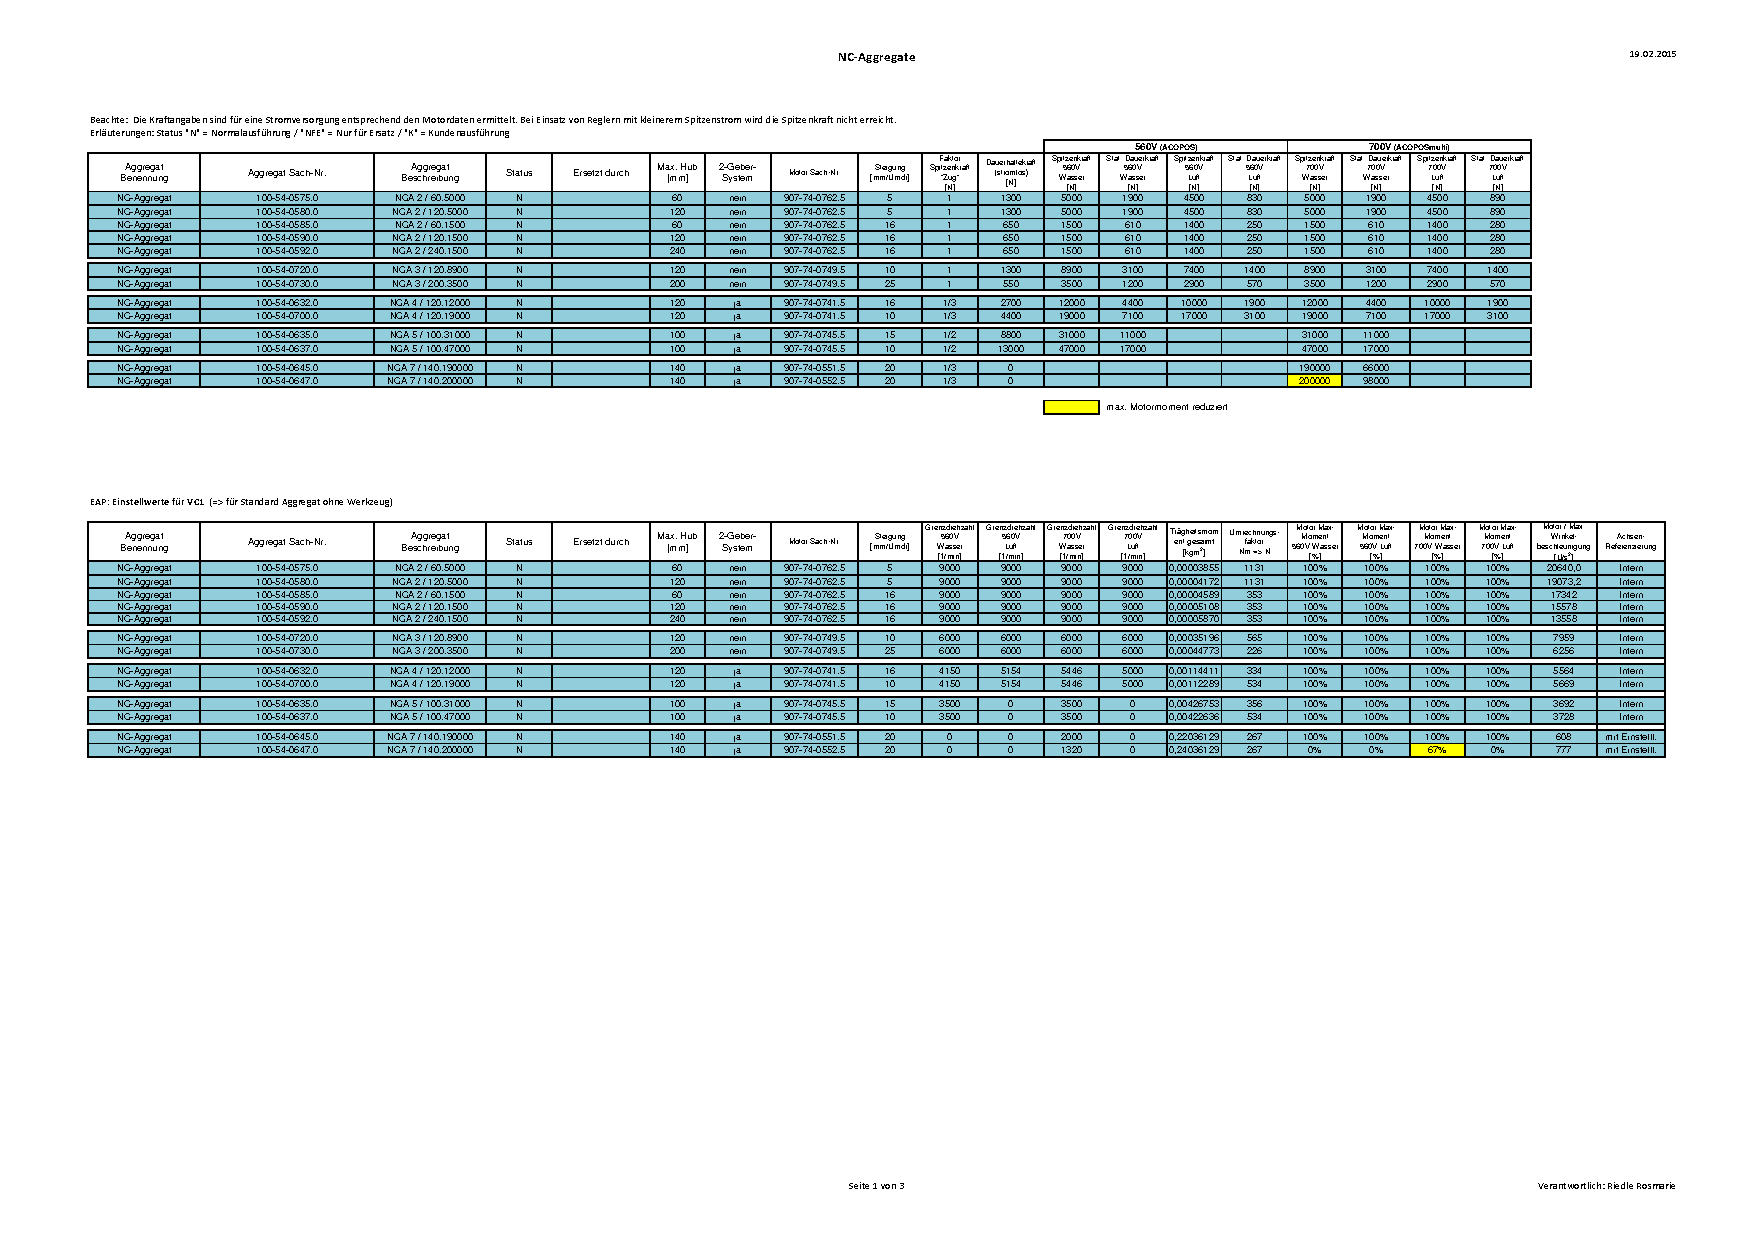
\includegraphics[page=1,angle=90,width=\textwidth]{anhang/Ueberblick_Ueber_NC_Aggregate.pdf}

\clearpage

\includegraphics[page=2,angle=270,width=\textwidth]{anhang/Ueberblick_Ueber_NC_Aggregate.pdf}

\clearpage

\includegraphics[page=3,angle=90,width=\textwidth]{anhang/Ueberblick_Ueber_NC_Aggregate.pdf}


\clearpage




\section{Übersicht über aufgetretene Fehler}\label{cha:Uebersicht_ueber_aufgetretene_Fehler}




\begin{itemize}
 \item konstruktive Fehler
 \begin{itemize}
    \item Kleber für Messlineal ist nicht für die ölhaltige Umgebung und Temperaturen vorgesehen
    \item Der konstruktive Fehler, dass Schmieröl in den Motor und anschließend in den Motorgeber gelangen kann, wurde bereits durch konstruktive Maßnahmen beseitigt. Allerdings sind noch einige Achsen mit dieser Schwachstelle im Umlauf. So ist in der nächsten Zeit mit weiteren Reklamationen aufgrund dieser Ursache zu rechnen.
 \end{itemize}
 
 
 
 
 
 \item Fertigungsfehler der Einzelkomponenten
 \begin{itemize}
    \item Immer wieder müssen nicht zeichnungsgemäß gefertigte Bauteile nachgearbeitet oder ausgetauscht werden. Dies führt zu erheblichen Verzögerungen während der Montage.
 \end{itemize}
 
 
 
 \item Fehler bei der Montage 
 \begin{itemize}
    \item Durch Fehler bei der Montage ergibt sich axiales Spiel, insbesondere durch nicht richtiges Anziehen der Spannmutter in der Pinole. Durch abändern der Montage Reihenfolge kann das falsche Anziehen der Spannmutter verhindert werden. Durch falsches Abstimmen der Abstimmscheibe kann es allerdings immer noch zu axialem Spiel kommen.
    \item Durch nicht richtig abgestimmte Abstimmscheiben kann es entweder zu axialem Spiel oder einer zu großen Vorspannung der Lager kommen.
 \end{itemize}
 
 
 
 
 \item fehlerhafte Programmierung
 \begin{itemize}
    \item Falsch programmierte Parameter treten immer wieder auf, da beim Einrichten eines neuen Werkzeuges alle Parameter für das Aggregat manuell eingegeben werden müssen. Dies führt immer wieder zu unerwarteten Fehlern und längeren Fehlersuchen.
 \end{itemize}
 
 
 \item nicht bestimmungsgemäßer Gebrauch
 \begin{itemize}
    \item Überlastung des Motors. Reklamation
    \item Gleitstein beschädigt (auf Block gefahren). Falsche Handhabung oder falsche Programmierung
 \end{itemize}
 
 
 
 
 \item nicht bestimmungsgemäße Instandhaltung
 \begin{itemize}
    \item Kühlkreislauf ist zugesetzt. Dies ist insbesondere ein Problem bei unsachgemäßen Umgang mit dem Kühlschmiermittel. Auch durch Späne oder sonstige Gegenstände in den Kühlkanälen ist der Durchfluss nicht sichergestellt.
 \end{itemize}
 
 
 \item Verschleiß und Alterungserscheinungen
 
 \clearpage
 
 \item nicht eindeutig zuordenbare Fehler
 \begin{itemize}
    \item Fressen bzw. vorher Verkratzen der Laufflächen der Pinole. Eine mögliche Ursache ist hier mangelnde Schmierung. Es ist bekannt, dass eine außermittige Belastung dieses Problem verschärft, genauso wie sehr kurze Verfahrbewegungen. so dass nicht der ganze Weg verfahren wird
    \item allgemeiner Fehler AMO-Messsystem (Reklamationsmanagementsystem)
    \item Defekt am Motor (Fehler b. Lieferanten) (Reklamationsmanagementsystem)
    \item Der Wellendichtring an der Pinole neigt des Öfteren dazu, kaputt zu gehen oder nicht die geforderte Dichtigkeit zu erreichen.
    \item Motor: Kühlsystem undicht (Reklamationsmanagementsystem)
    \item Haltebremse versagt
 \end{itemize}
\end{itemize}



% \includepdf[pages=-,angle=270]{anhang/Ueberblick_Ueber_NC-Aggregate.pdf}
%\includepdf[pages=1,pagecommand=\section{Überblick über NC-Aggregate}, angle=270,scale=0.8]{anhang/Ueberblick_Ueber_NC-Aggregate.pdf}

%\includepdf[pages=2,pagecommand={}, angle=270, noautoscale=true, width=\textwidth]{anhang/Ueberblick_Ueber_NC-Aggregate.pdf}

%\includepdf[pages=3,pagecommand={}, angle=270,noautoscale=true, width=\textwidth]{anhang/Ueberblick_Ueber_NC-Aggregate.pdf}



%\end{comment}


% Eidesstattliche Erklärung
%% Die eidesstattliche Erklärung mit Unterschrift
\chapter*{Erklärung der Urheberschaft}\addcontentsline{toc}{chapter}{Erklärung der Urheberschaft}

Ich erkläre hiermit an Eides statt, dass ich die vorliegende Arbeit
ohne Hilfe Dritter und ohne Benutzung anderer als der angegebenen
Hilfsmittel angefertigt habe; die aus fremden Quellen direkt oder
indirekt übernommenen Gedanken sind als solche kenntlich gemacht. Die
Arbeit wurde bisher in gleicher oder ähnlicher Form in keiner anderen
Prüfungsbehörde vorgelegt und auch noch nicht veröffentlicht.


\vspace{4cm}

\hspace{2cm} Ort, Datum \hfill Unterschrift \hspace{2cm}

\end{document}